\documentclass[a4paper,11pt]{article}
\usepackage{jinstpub} % for details on the use of the package, please see the JINST-author-manual
\usepackage{booktabs}
\usepackage{subcaption}
\usepackage{siunitx}
\usepackage{amsmath}
\usepackage[section]{placeins}

% --- Float packing: reduce whitespace on pages with figures/tables ---
\renewcommand{\topfraction}{0.9}        % up to 90% of page top for floats
\renewcommand{\bottomfraction}{0.9}     % up to 90% of page bottom for floats
\renewcommand{\textfraction}{0.07}      % at least 7% text on a mixed page
\renewcommand{\floatpagefraction}{0.75} % float-only page must be 75% full
\setcounter{topnumber}{4}               % max 4 floats at page top
\setcounter{bottomnumber}{3}            % max 3 floats at page bottom
\setcounter{totalnumber}{6}             % max 6 floats per page total
\setlength{\floatsep}{8pt plus 2pt minus 2pt}      % between consecutive floats
\setlength{\textfloatsep}{10pt plus 3pt minus 2pt}  % between float and text
\setlength{\intextsep}{8pt plus 2pt minus 2pt}      % around in-text floats
\setlength{\bibsep}{3pt plus 1pt minus 1pt}         % inter-reference spacing

\title{\boldmath Origami-Folded Sensor Geometries for Cylindrical Tracking Detectors: A \textsc{Geant4} Comparison}

\author{Kanishk Sharma}
\affiliation{Air Force Bal Bharti School}

% E-mail address: corresponding author
\emailAdd{kanishk@mathsdiscourse.com}

\abstract{Cylindrical tracking detectors in high-energy physics are traditionally built from flat silicon sensor tiles arranged around a support barrel. Flat silicon modules cannot bend easily, so covering a cylindrical surface with flat tiles requires a trade-off between leaving inactive detection gaps (dead zones) and creating tile overlaps that add unwanted material. Recent vertex detector designs address this issue using tilted sensor modules or bent, stitched silicon (such as ALICE ITS3). Here, we investigate an alternative approach: origami-folded detector structures. We present what appears to be the first systematic \textsc{Geant4} comparison of three cylindrical origami fold families --- Cylindrical Miura-ori, Yoshimura, and Kresling --- against a matched flat-tiled barrel control for charged-particle tracking.

Each geometry was modeled parametrically in Python and simulated in \textsc{Geant4} with differentiated materials (discrete rigid silicon tiles on a continuous flexible Kapton substrate). Across $500{,}000$ primary $5\text{ GeV}/c\ \pi^+$ events per configuration with a $3.0\text{ mm}$ vertex spread, all three fold geometries achieved higher geometric hit acceptance than the flat-tiled control barrel, accompanied by increases in radiation-length traversal. Kresling yielded the largest acceptance gain ($+2.36$ percentage points, $p < 10^{-10}$, Cohen's $h = +0.066$) with a $+5.69\%$ increase in mean $X_0$. Yoshimura exhibited a $+1.30$ percentage-point acceptance gain ($p < 10^{-9}$, Cohen's $h = +0.035$) with the largest material increase ($+8.01\%$ in $X_0$). Miura-ori exhibited the lowest material penalty, closely matching the control ($+1.88\%$ in $X_0$), with a modest acceptance gain ($+0.49$ percentage points, $p < 10^{-7}$, Cohen's $h = +0.013$).

These candidate structures define a distinct Pareto frontier rather than a single optimal design. Spatial hit-density analysis reveals that Yoshimura and Kresling concentrate their acceptance gains primarily in localized seam-overlap regions, retaining relative under-coverage fractions ($1.86\%$ and $1.45\%$ of $(\theta, z)$ bins with $R < 0.5$, respectively). Conversely, Miura-ori provides near-uniform spatial coverage with the lowest relative under-coverage fraction ($0.04\%$). Parameter sweeps over facet count $N$, fold angle $\theta$, vertex-position distributions, independent five-run replications ($\mathrm{SD}_A \le 0.05$~pp), and multiple-scattering validation against the Highland formula confirm the statistical robustness of these findings.

A parallel evaluation at $50\ \mu\text{m}$ silicon thickness --- matching the ALICE ITS3 benchmark --- indicates that the geometric acceptance advantage of folding remains essentially the same at lower sensor thickness, while total material traversal scales down by $\sim 4.8\times$. Compared against ITS3's bent sensor baseline at matched physical scope, flat-faceted tessellations retain a modest silicon-only material penalty ($+0.010$--$0.016$ pp in $X/X_0$) due to non-normal local incidence angles. Origami folding therefore enhances geometric acceptance relative to conventional tiled barrels at any matched sensor thickness, redistributing the dead-zone and overlap trade-off across distinct Pareto-optimal configurations.}

\keywords{Performance of High Energy Physics Detectors, Simulation methods and programs, Radiation calculations, Analysis and statistical methods}

\begin{document}
\maketitle
\flushbottom

\section{Introduction}
\label{sec:intro}

Barrel-shaped tracking detectors in particle physics are conventionally built from flat silicon sensor modules mounted on a cylindrical support structure. Crystalline silicon is brittle and does not bend easily. Consequently, tiling a cylindrical envelope with flat modules creates a direct trade-off: leaving gaps between adjacent tiles leaves inactive detection areas (dead zones), whereas overlapping tiles introduces extra material that increases multiple scattering and degrades tracking resolution.

Detector optimization efforts have predominantly concentrated on ultra-light carbon composite supports, micro-channel cooling, and high-density flexible interconnects, rather than modifying the underlying planar tiling topology.

Recent vertex detector architectures have developed innovative strategies to mitigate these geometric constraints. The ALICE ITS3 upgrade utilizes ultra-thin ($40$--$50\ \mu\text{m}$) stitched CMOS sensors bent into cylindrical half-layers, eliminating active sensor seams entirely within the tracking layers~\cite{ALICE2024, Sonneveld2023}. The LHCb Upstream Tracker combines rigid silicon sensors with a continuous flexible Kapton substrate for electrical routing and mechanical integration~\cite{Lionetto2014}. The CMS Phase-2 Outer Tracker employs a tilted-module geometry in the tracker barrel, inclining flat sensor modules along the beam axis to optimize track incidence angles and close acceptance gaps~\cite{CMS2017}.

While these methods show the advantages of non-standard geometries, origami-folded designs have not yet been evaluated systematically for tracking detectors. Origami folding allows a continuous sheet to form a pattern of flat panels connected along fold lines, enabling compact storage followed by deployment into a cylindrical geometry.

This work presents what appears to be the first systematic \textsc{Geant4} comparison of three cylindrically deployable origami fold families --- Cylindrical Miura-ori~\cite{Miura1985}, Yoshimura~\cite{Yoshimura1955}, and Kresling~\cite{Kresling2008} --- against a conventional planar-tiled barrel control of identical envelope dimensions ($R = 40\text{ mm}$, $L = 120\text{ mm}$).

The central question investigated is whether, for a fixed cylindrical envelope, origami folding can improve geometric tracking acceptance without imposing an intolerable radiation-length penalty relative to conventional tiling. The three fold geometries were generated parametrically in Python and simulated in \textsc{Geant4} using explicitly differentiated material representations (rigid silicon tiles on a continuous Kapton backing). A flat planar slab model was simulated in parallel to validate radiation-length scoring and multiple-scattering distributions against the Highland formula.

The radiation-length values reported here correspond to the active sensor and flexible substrate stack. They do not represent a complete detector material budget; mechanical supports, cooling infrastructure, cabling, and readout electronics are intentionally excluded to isolate pure geometric effects.

\FloatBarrier
\section{Methods}
\label{sec:methods}

\subsection{Candidate and Control Geometries}
\label{sec:geometries}

Four cylindrical envelopes sharing an identical outer bounding radius ($R = 40\text{ mm}$) and active length ($L = 120\text{ mm}$) were constructed and simulated (Figure~\ref{fig:geometries}):
\begin{itemize}
    \item \textbf{Barrel reference} --- A conventional flat-tile cylindrical barrel serving as the control baseline. Its planar faceted joints establish the baseline dead-zone and overlap performance.
    \item \textbf{Cylindrical Miura-ori} --- The classic Miura-ori herringbone parallelogram tessellation~\cite{Miura1985} mapped onto a cylindrical envelope.
    \item \textbf{Yoshimura} --- The diamond-pattern triangular cylindrical tessellation characteristic of thin-shell axial buckling~\cite{Yoshimura1955}.
    \item \textbf{Kresling} --- The chiral, triangulated cylinder exhibiting coupled axial compression and rotation~\cite{Kresling2008}.
\end{itemize}

\begin{figure}[!htbp]
\centering
\begin{subfigure}[b]{0.46\textwidth}
    \centering
    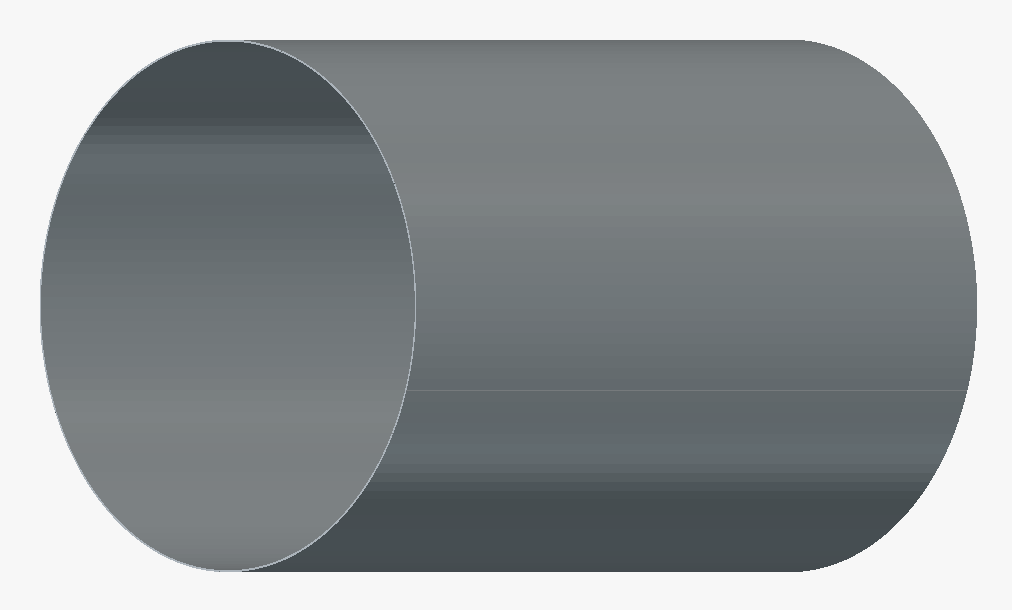
\includegraphics[width=\textwidth]{figures/fig1_barrel.png}
    \caption{Barrel reference (fine-tiled)}
    \label{fig:geom_barrel}
\end{subfigure}
\hfill
\begin{subfigure}[b]{0.46\textwidth}
    \centering
    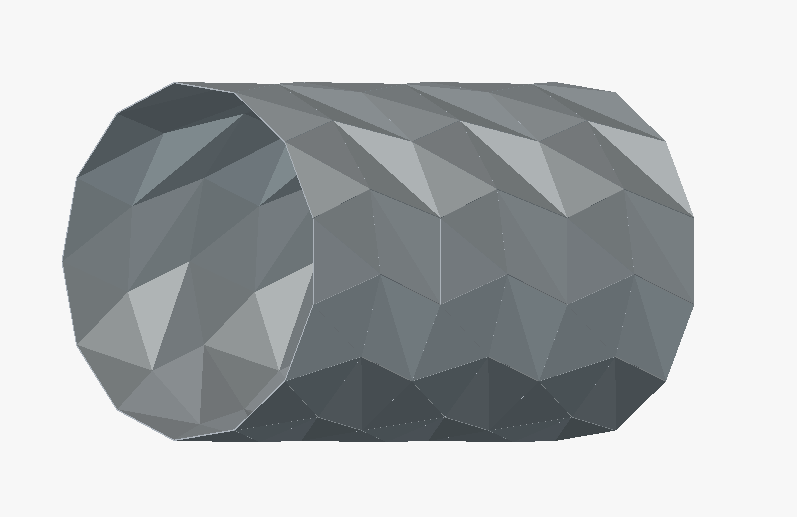
\includegraphics[width=\textwidth]{figures/fig1_miura.png}
    \caption{Miura-ori}
    \label{fig:geom_miura}
\end{subfigure}\\[0.2em]
\begin{subfigure}[b]{0.46\textwidth}
    \centering
    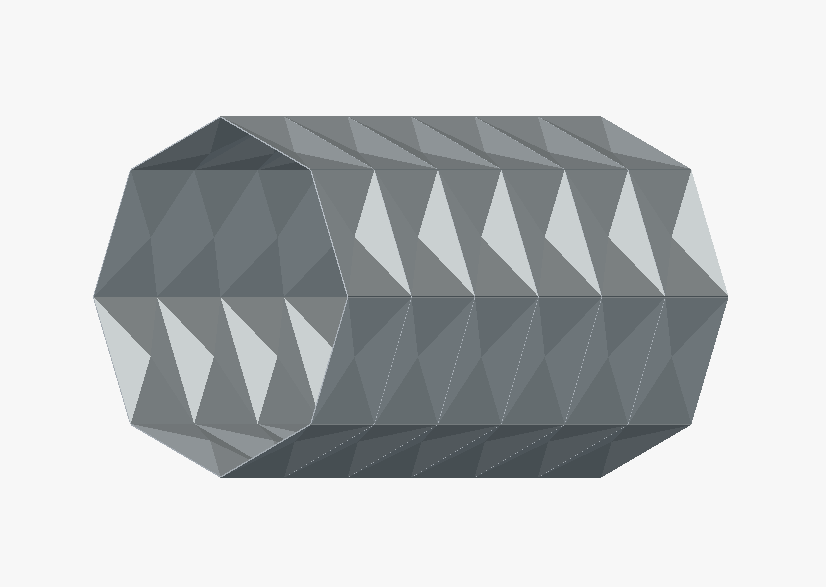
\includegraphics[width=\textwidth]{figures/fig1_yoshimura.png}
    \caption{Yoshimura}
    \label{fig:geom_yoshimura}
\end{subfigure}
\hfill
\begin{subfigure}[b]{0.46\textwidth}
    \centering
    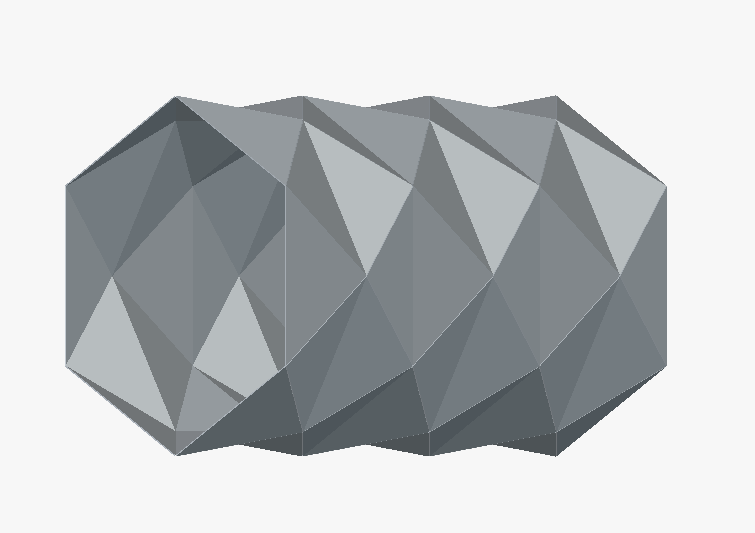
\includegraphics[width=\textwidth]{figures/fig1_kresling.png}
    \caption{Kresling}
    \label{fig:geom_kresling}
\end{subfigure}
\caption{The four simulated detector geometries in their fully deployed configurations at matched radius ($R = 40\text{ mm}$) and length ($L = 120\text{ mm}$)}
\label{fig:geometries}
\end{figure}

Each geometry uses the same two-material layer stack. Silicon is the rigid sensor material ($300\ \mu\text{m}$ thickness); however a silicon sensor cannot be bent through a sharp crease without cracking, thus any physically realizable folded sensor sheet requires a flexible backing. Kapton (polyimide, $50\ \mu\text{m}$ thickness) provides this backing, with rigid silicon mounted on the flat facets. This mechanical distinction is part of why these fold patterns are a viable design direction.

Every geometry was built to the same fixed physical envelope and material stack, so comparisons are meaningful. Table~\ref{tab:geom_params} summarizes the properties:

Crucially, the silicon and Kapton layers are generated using distinct geometric offset schemes from the underlying polygonal mesh:
\begin{enumerate}
    \item \textbf{Silicon layer (per-facet normal offset):} Each polygonal facet is extruded along its individual face normal and boolean-unioned into a watertight solid. This accurately reflects discrete, rigid sensor tiles whose edges terminate at fold boundaries.
    \item \textbf{Kapton layer (per-vertex area-weighted normal offset):} The flexible substrate is extruded along shared, vertex-averaged normals, producing a seamless, continuous backing across fold lines without artificial wedge gaps or overlap tearing.
\end{enumerate}


The nominal geometric parameters for each structure are summarized in Table~\ref{tab:geom_params}. The fine-tiled barrel column count ($141$ columns) is determined by an inscribed sagitta tolerance of $s \le 0.01\text{ mm}$, ensuring it approximates a smooth cylinder. The fold structures use an axial unit-cell repeat scale of $20\text{ mm}$.

\begin{table}[!htbp]
\centering
\caption{Geometric parameters and material budget of the simulated structures at fixed $R = 40\text{ mm}$, $L = 120\text{ mm}$, $300\ \mu\text{m}$ Si, $50\ \mu\text{m}$ Kapton. Active area is the total mid-surface sensor area; $A_{\text{cyl}} = 2\pi R L = 301.59\text{ cm}^2$. Masses at $\rho_{\text{Si}} = 2.329\text{ g/cm}^3$, $\rho_{\text{Kapton}} = 1.420\text{ g/cm}^3$.}
\label{tab:geom_params}
\smallskip
\resizebox{\textwidth}{!}{
\begin{tabular}{llccccc}
\toprule
Geometry & Segmentation / Panel count & Fold parameter & $A_{\text{active}}$ (cm$^2$) & $A/A_{\text{cyl}}$ & $m_{\text{Si}}$ (g) & $m_{\text{Kapton}}$ (g) \\
\midrule
Barrel reference (fine-tiled)   & 6 rows $\times$ 141 cols (846 quads) & ---                                            & 301.57 & 0.9999 & 21.07 & 2.14 \\
Barrel reference (coarse-tiled) & 12 rows $\times$ 24 cols (288 quads) & ---                                            & 301.50 & 0.9997 & 21.07 & 2.14 \\
Miura-ori                       & 6 rows $\times$ 13 cols              & Crease angle $\alpha = 45^\circ$               & 293.20 & 0.9722 & 20.49 & 2.08 \\
Yoshimura                       & 6 rings $\times$ 8 facets            & Fold angle $\theta = 30^\circ$ ($\pi/6$ rad)   & 334.82 & 1.1102 & 23.39 & 2.38 \\
Kresling                        & 6 layers $\times$ 6 sides            & Twist angle $\theta = 30^\circ$/layer          & 312.44 & 1.0360 & 21.83 & 2.22 \\
\bottomrule
\end{tabular}
}
\end{table}
The fine-tiled column count (141) comes from a geometric sagitta tolerance --- the maximum allowed deviation of a flat panel from the true 40 mm circle, set to 0.01 mm --- chosen so the fine-tiled barrel approximates a smooth cylindrical shell rather than a visibly faceted polygon. We also compare it to a second, coarse-tiled barrel configuration (12 rows $\times$ 24 cols, 288 quads, chosen independently of any tolerance criterion) specifically to check how much the barrel's own tile density affects its acceptance and mean path length. That coarse configuration isn't a candidate reference geometry on its own and is just used here.

As shown in Table~\ref{tab:geom_params}, the non-planar corrugations of fold geometries modify their total physical sensor area relative to the smooth cylinder. Yoshimura ($+11.02\%$) and Kresling ($+3.60\%$) have more active silicon area than the barrel, which both increases the number of intercepted tracks and raises the material traversed by each --- the two effects are not independent. Miura-ori's inscribed facets project slightly inside the envelope ($97.22\%$ of $A_{\text{cyl}}$), giving it less silicon mass than the barrel and explaining its smaller material penalty ($+1.88\%$ in $X_0$). These area ratios provide the geometric denominator for interpreting the acceptance and radiation-length results in Section~\ref{sec:results}.

\FloatBarrier
\subsection{Purpose of the Barrel Reference and Baseline Selection}
\label{sec:baseline}

The barrel reference exists to answer a specific question: how much of the under-coverage and radiation-length behavior seen in a fold geometry comes from folding, and how much would be present anyway in any cylindrical detector built at that radius? Without a matched-radius, matched-material control, a fold geometry's under-coverage fraction or radiation-length traversal has no reference point against which it can be judged. A metric such as the fraction of under-covered bins only becomes meaningful once it is compared with what a conventional detector at the same radius would show.

The barrel reference was therefore held to the same radius, the same silicon and substrate layer thicknesses, and the same particle beam and event count as the three fold geometries, so that the only geometric variable left is the presence and shape of the fold lines. The barrel is thus the baseline against which the rest of the paper is measured, rather than one option among four being ranked independently.

For the particle simulations, pions with a momentum of $5\text{ GeV}/c$ were chosen. This has three effects:

\begin{enumerate}

    \item It ensures that the energy loss recorded by the scorer reflects the geometry a track passes through---path length and material---rather than energy-dependent stopping-power effects near the Bragg-like rise at low momentum, which would complicate any comparison between geometries with different effective thicknesses at a given incidence angle.

    \item Relativistic effects ensure that pions do not undergo in-flight decay over the required duration.

    \item Even considering hadronic interactions with silicon, the simulation explicitly only counts the primary particles towards the acceptance numbers, not secondary particles. This prevents secondary particles from masking geometric gaps in the detector.

\end{enumerate}
\subsection{Simulation Pipeline}
\label{sec:pipeline}

All geometries are derived from their mathematical formulae and then modeled parametrically in Python. These geometries are then exported to GDML (Geometry Description Markup Language) using explicitly indexed \texttt{<tessellated>} solids and parsed directly by \textsc{Geant4}~\cite{Agostinelli2003}, guaranteeing strict watertightness and preventing navigation track-trapping errors.

\begin{figure}[!htbp]
\centering
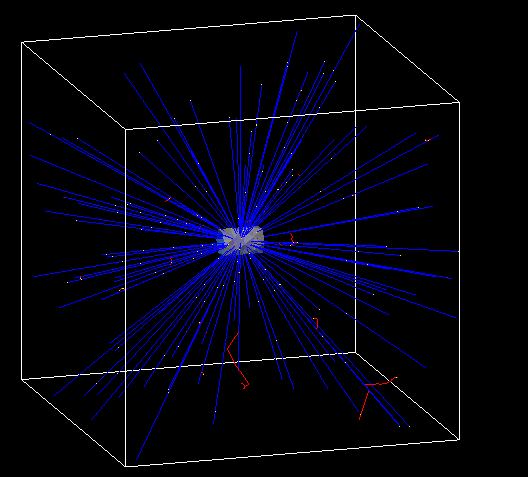
\includegraphics[width=0.65\textwidth]{figures/fig2_event_display.png}
\caption{Three-dimensional \textsc{Geant4} event display showing primary $5\text{ GeV}/c\ \pi^+$ tracks (blue) emitted isotropically from the central interaction vertex through the detector volume, with secondary hadronic tracks indicated in red.}
\label{fig:event_display}
\end{figure}

The primary particle generator emits particles isotropically over $4\pi$ solid angle. To accurately reflect collider beam-spot distributions, the vertex is sampled from a three-dimensional Gaussian distribution with $\sigma_x = \sigma_y = \sigma_z = 3\text{ mm}$ centered at the origin (Figure~\ref{fig:event_display}). Since isotropic emission over solid angle scales as $\sin\theta$, equatorial polar angle bins ($\theta \approx 90^\circ$) receive greater track density than forward/backward bins; since all geometries share identical source definitions, relative comparisons remain strictly unbiased.

Each run consists of $500{,}000$ primary events per configuration. Step-level sensitive detectors record active volume hits, true traversed 3D path lengths in silicon and Kapton, deposited energy, emission polar angle $\theta$, and local surface incidence angle $\theta_{\text{local}}$.

\subsection{Evaluation Metrics}
\label{sec:metrics}

Four primary performance metrics are evaluated:
\begin{itemize}
    \item \textbf{Acceptance fraction ($A$):} The proportion of primary particles producing at least one hit in active silicon ($A = N_{\text{hit}} / N_{\text{total}}$). To ensure clean geometric isolation, all scoring is restricted strictly to primary particle tracks ($\text{parentID} = 0$), filtering out secondary hadronic fragments and delta rays so that both acceptance and multiple-scattering angles reflect the true primary trajectory.
    \item \textbf{Mean and median material traversal in radiation lengths ($X/X_0$):} Step-level path lengths scaled by material radiation lengths ($X_0(\text{Si}) = 9.366\text{ cm}$, $X_0(\text{Kapton}) = 28.575\text{ cm}$).
    \item \textbf{Local hit-density enhancement ratio ($R(\theta, z)$):} The per-bin ratio of fold geometry hit density to the barrel reference across a 2D $(\theta, z)$ grid.
    \item \textbf{Relative under-coverage fraction ($f_{\text{under}}$):} The fraction of geometrically covered $(\theta, z)$ phase space bins where the fold hit density falls significantly below the planar baseline ($R(\theta, z) < 0.5$). This metric quantifies local suppression of hit density relative to the barrel; it represents relative under-density rather than absolute detection blindness. Sweeping the detection threshold from $0$ to $1$ (Section~\ref{sec:deadzone_pareto}) confirms that true zero-hit voids ($f_{\text{zero}} \approx 0$) are virtually absent within the active tracking volume, with under-coverage confined to moderate efficiency dips near fold seams.
\end{itemize}

\subsection{Statistical Treatment}
\label{sec:statistics}

Acceptance fraction is a proportion of a binomial count (hits out of 500{,}000 trials), so its standard error is computed directly from binomial statistics:
\begin{equation}
\label{eq:se_binomial}
SE_A = \sqrt{\frac{A(1-A)}{N}}\,,
\end{equation}
where $A$ is the acceptance fraction and $N$ is the number of primary events. Mean path length in $X_0$ is likewise reported with a standard error of the mean,
\begin{equation}
\label{eq:sem_path}
SEM = \frac{s}{\sqrt{N_{\mathrm{hit}}}}\,,
\end{equation}
where $s$ is the sample standard deviation of the per-event path length over hit-producing tracks and $N_{\mathrm{hit}}$ is the number of hits.

For any pairwise comparison---a fold geometry against the barrel, or against another fold geometry---the two standard errors combine as
\begin{equation}
\label{eq:se_diff}
SE_{\mathrm{diff}} = \sqrt{SE_1^2 + SE_2^2}\,,
\end{equation}
with the corresponding test statistic given by
\begin{equation}
\label{eq:z_score}
z = \frac{\mathrm{diff}}{SE_{\mathrm{diff}}}\,.
\end{equation}
For acceptance comparisons, $\mathrm{diff}=A_1-A_2$; for path-length comparisons, the corresponding difference in mean path length is used. Whenever two different geometries are compared, a Holm--Bonferroni correction is applied across the relevant family of tests rather than reading each $p$-value against an uncorrected threshold.

Cohen's $h$, a standardized effect size for comparing two proportions, is reported alongside pairwise acceptance differences:
\begin{equation}
\label{eq:cohen_h}
h = 2\arcsin\sqrt{A_1} - 2\arcsin\sqrt{A_2}\,.
\end{equation}
In large-sample collider simulations ($N = 500{,}000$ per geometry), even modest differences in acceptance produce very large test statistics ($z$-scores and $t$-values) due to the small standard error ($\mathrm{SE} \propto 1/\sqrt{N}$). Cohen's $h$ is therefore reported as a scale-free measure of effect size.

Physical reproducibility is established through five independent simulation runs per geometry with distinct pseudo-random seeds. For each metric, we report the sample mean, standard deviation ($\mathrm{SD}$), standard error of the mean ($\mathrm{SEM}$), and 95\% confidence intervals. Pairwise comparisons across independent runs are evaluated using Welch's two-sample $t$-test with Holm--Bonferroni correction across the family of comparisons. The small run-to-run variation ($\mathrm{SD}_A \le 0.05$~pp, Table~\ref{tab:multirun_results}) confirms that the observed acceptance differences reflect true geometric performance rather than Monte Carlo fluctuations.

\subsection{Radiation-Length and Multiple-Scattering Validation}
\label{sec:validation}

The \textsc{Geant4} step-level material accumulator was validated against an analytical planar slab model at normal incidence ($\theta_{\text{local}} = 0^\circ$):
\begin{align}
(X/X_0)_{\text{Si}} &= \frac{0.03\text{ cm}}{9.366\text{ cm}} = 3.2031 \times 10^{-3}\,, \label{eq:x0_si} \\
(X/X_0)_{\text{Kapton}} &= \frac{0.005\text{ cm}}{28.575\text{ cm}} = 1.7498 \times 10^{-4}\,, \label{eq:x0_kapton} \\
(X/X_0)_{\text{total}} &= 3.2031 \times 10^{-3} + 1.7498 \times 10^{-4} = 3.3781 \times 10^{-3}\,. \label{eq:x0_total}
\end{align}
Across five independent validation runs ($2{,}000$ events each), the simulated mean path length was $(3.3779 \pm 0.0001) \times 10^{-3}\ X_0$, matching analytical theory to within $-0.005\%$ ($z \approx -1.6$, non-significant).

Multiple Coulomb scattering was independently checked against the Highland formula~\cite{Highland1975, Lynch1991}:
\begin{equation}
\label{eq:highland}
\theta_0 = \frac{13.6\text{ MeV}}{\beta c p} z_0 \sqrt{\frac{x}{X_0}} \left[ 1 + 0.038 \ln \left( \frac{x}{X_0} \right) \right]\,.
\end{equation}
A first attempt, which was just a single application of the formula to the full simulated scattering-angle distribution, gave a puzzling result: $\theta_{0,\text{sim}} / \theta_{0,\text{Highland}} = 0.537 \pm 0.008$ across 20 momentum--geometry configurations ($p \in [0.5, 10.0]\text{ GeV}/c$) --- a large, consistent shortfall with no physical explanation attached to it.

However, this traced back to the fitting method --- i.e., the model chosen --- not to failed runs. Since the particles are fired from an isotropic source, around a solid angle of $4\pi$, the resulting scattering angle is not Gaussian. Plotting the probability density of the simulated space-scattering angle for the barrel reference at all five momenta on a log-log scale reveals something interesting: overlaying the corresponding Highland predictions for each momentum shows the two curves moving together at small angle, but after roughly 3--4 times the Highland $\theta_0$, they diverge sharply. The simulated distribution flattens into a power-law tail that extends more than two decades past where the Highland curve has already dropped by several orders of magnitude. A plain unconstrained Gaussian fit to a distribution shaped like this is pulled wide by that tail --- exactly the kind of bias a heavy-tailed distribution produces on a naive width estimator, and exactly why the first-pass fit undershot Highland by roughly a factor of two rather than agreeing with it.

\paragraph{Core-plus-tail fit.} The scattering-angle distribution was refit as an explicit two-component mixture model, using the 3-D space-scattering angle directly (Section~\ref{sec:pipeline}):
\begin{equation}
\label{eq:core_tail_mixture}
p(\theta) = (1 - f) \cdot \mathrm{Rayleigh}(\theta; \sigma) + f \cdot \mathrm{PowerLaw}(\theta; \theta_{\min} = 3\sigma, \alpha)\,, \qquad \theta > 0\,.
\end{equation}
The core is modeled as a Rayleigh distribution rather than a simple Gaussian, which is the correct choice for a space angle: if the two orthogonal plane deflections are each Gaussian with width $\theta_0$ (Highland's own quantity), their magnitude follows a Rayleigh distribution with scale parameter $\theta_0$, with no additional conversion factor required. The tail is modeled in accordance with Rutherford's power law, $dN/d\theta \propto \theta^{-\alpha}$, beyond a tail-onset boundary fixed at three times the fitted core width ($\theta_{\min} = 3\sigma$), tying the tail region to the fit's own core scale rather than to a hand-picked cutoff. All three free parameters ($\sigma$, tail fraction $f$, and tail index $\alpha$) were fitted simultaneously using unbinned maximum-likelihood estimation against the full per-event scattering-angle sample ($N_{\text{hit}} > 4.1 \times 10^5$ events per configuration). Due to the enormous statistical power of the dataset, formal binned $\chi^2/\text{dof}$ goodness-of-fit values are sensitive to minute sub-percent level distribution discrepancies (Table~\ref{tab:highland_mixture_fits}), while the fitted parameter values ($\sigma/\theta_{0,\text{Highland}} \approx 0.93$, $\alpha \approx 3.0$) demonstrate stable, physically consistent agreement. This is the standard decomposition technique for multiple-scattering distributions in the HEP literature.

Refit this way, $\sigma / \theta_{0,\text{Highland}}$ (the fitted Rayleigh core scale over the Highland prediction) averages $0.930 \pm 0.003$ across all four geometries and all five momenta (Figure~\ref{fig:scattering_mixture}, top right; full values in Table~\ref{tab:highland_mixture_fits}) --- a stable, roughly 7\% shortfall, not a factor-of-two one, ranging only from 0.924 to 0.935 across the full 20-point dataset. A weak downward trend with momentum is visible in the data (Pearson $r = -0.42$, $p \approx 0.06$ across the 20 points) but does not reach conventional significance at this sample size, and in any case the entire swept range spans less than a 1.2-percentage-point band (0.924--0.935) --- small enough, relative to the $\sim$7\% offset itself, that it does not change the interpretation below. Figure~\ref{fig:scattering_mixture}(b) confirms the underlying shape stability directly for the barrel reference: rescaling both axes by Highland's own $\theta_0$ (angle on the $x$-axis, density on the $y$-axis, both in $\theta_0$-natural units) collapses all five momenta onto a single curve, meaning the whole angular distribution --- core and tail together --- obeys essentially the same shape at every momentum tested. That collapse is itself informative: whatever is producing the residual $\sim$7\% gap and the power-law tail is close to a scale-invariant property of the geometry, not a strongly momentum-dependent effect that a small-angle formula would be expected to miss more or less of at different momenta.

\paragraph{The tail itself matches Rutherford single scattering.} The fitted tail power index $\alpha$ averages $2.999 \pm 0.046$ across all 20 points (Figure~\ref{fig:scattering_mixture}, bottom right; Table~\ref{tab:highland_mixture_fits}) --- indistinguishable, to within fit uncertainty, from the value predicted by single Rutherford scattering off individual nuclei. The differential cross section for Rutherford scattering falls as $d\sigma/d\Omega \propto \theta^{-4}$ at small angle; converting from solid angle to a 1-D angular density via the Jacobian $d\Omega = 2\pi \sin\theta\, d\theta \approx 2\pi\theta\, d\theta$ gives $dN/d\theta \propto \theta^{-3}$ --- i.e., $\alpha = 3$, matching the fitted tail slope directly, and matching it at every geometry and every momentum tested, not just on average. Despite comprising only 3.3--3.9\% of events at any given configuration, this tail dominates the overall variance: Figure~\ref{fig:scattering_mixture_summary} shows the tail supplies 86.5\% of the total $\sum\theta^2$ on average (range 81.9--89.7\%) across the full dataset, for every geometry. A naive RMS-based width estimate is therefore almost entirely a measurement of the rare single-scatter tail, not of the multiple-scattering core Highland's formula describes --- the same conclusion reached independently from first principles on the raw per-event data (Appendix~\ref{sec:appendix_highland}).

\paragraph{Interpretation.} Two effects are cleanly separated by this refit, where the original single-Gaussian comparison conflated them into one confusing number:
\begin{enumerate}
\item The Rayleigh \textbf{core} --- the many-small-deflections regime Highland's formula was derived for --- agrees with Highland to within $\sim$7\% ($\sigma/\theta_{0,\text{Highland}} = 0.930 \pm 0.003$), consistently across all four geometries and the full momentum range tested. This is the level of agreement expected between a full simulation and Highland's own empirical approximation to it, and is well within Highland's stated accuracy for $x/X_0$ in the range used throughout this study.
\item A \textbf{Rutherford single-scattering tail}, with the theoretically correct power index ($\alpha = 2.999 \pm 0.046$), sits on top of the core, is small in event count (3.3--3.9\%) but dominates the raw variance (81.9--89.7\% of $\sum\theta^2$), and is a real physical feature of Coulomb scattering that Highland's formula was never designed to capture --- Highland is explicitly a small-angle multiple-scattering approximation, not a full-distribution model.
\end{enumerate}

The 0.537 figure from the initial single-Gaussian comparison was therefore a measurement of a fit dominated by tail events it wasn't modeling, not a measurement of core agreement with Highland. Refit with a mixture model that separates the two components, the simulation's core matches Highland's small-angle prediction to within the level of agreement the formula's own derivation would lead one to expect, and the residual structure past the core is physical, not a simulation artifact --- its power index is the textbook Rutherford value, its shape is stable across four different geometries, and it collapses onto a single universal curve in Highland-rescaled units across the full momentum range.

\begin{figure}[!htbp]
\centering
\begin{subfigure}[b]{0.48\textwidth}
    \centering
    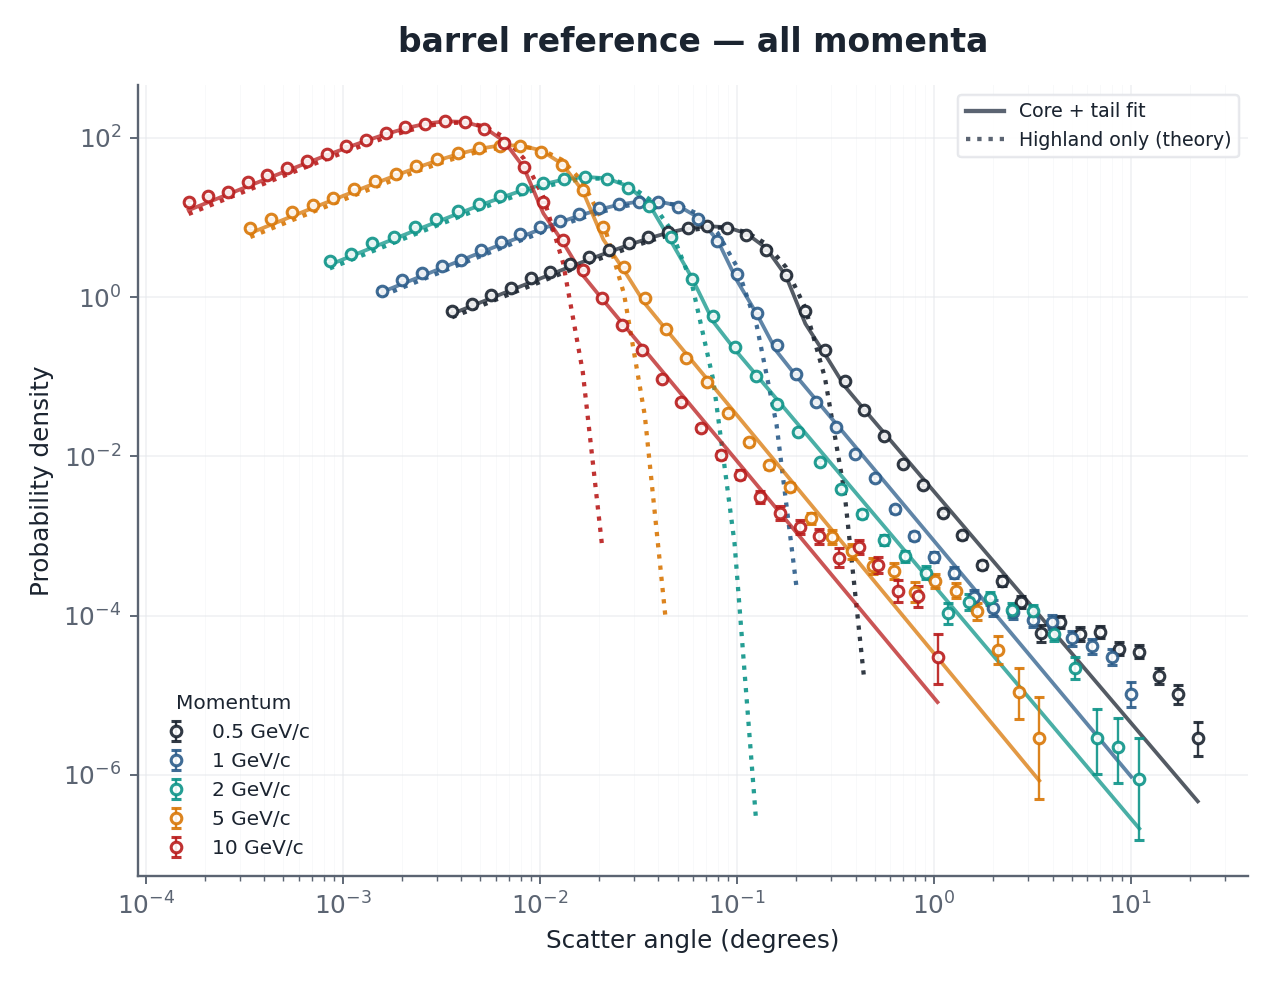
\includegraphics[width=\textwidth]{figures/fig_scattering_mixture_barrel_density.png}
    \caption{Barrel-reference scattering-angle probability density across all five simulated momenta (0.5--10~GeV/$c$), mixture fit (solid) vs.\ Highland-only Rayleigh prediction (dotted)}
    \label{fig:mixture_a}
\end{subfigure}
\hfill
\begin{subfigure}[b]{0.48\textwidth}
    \centering
    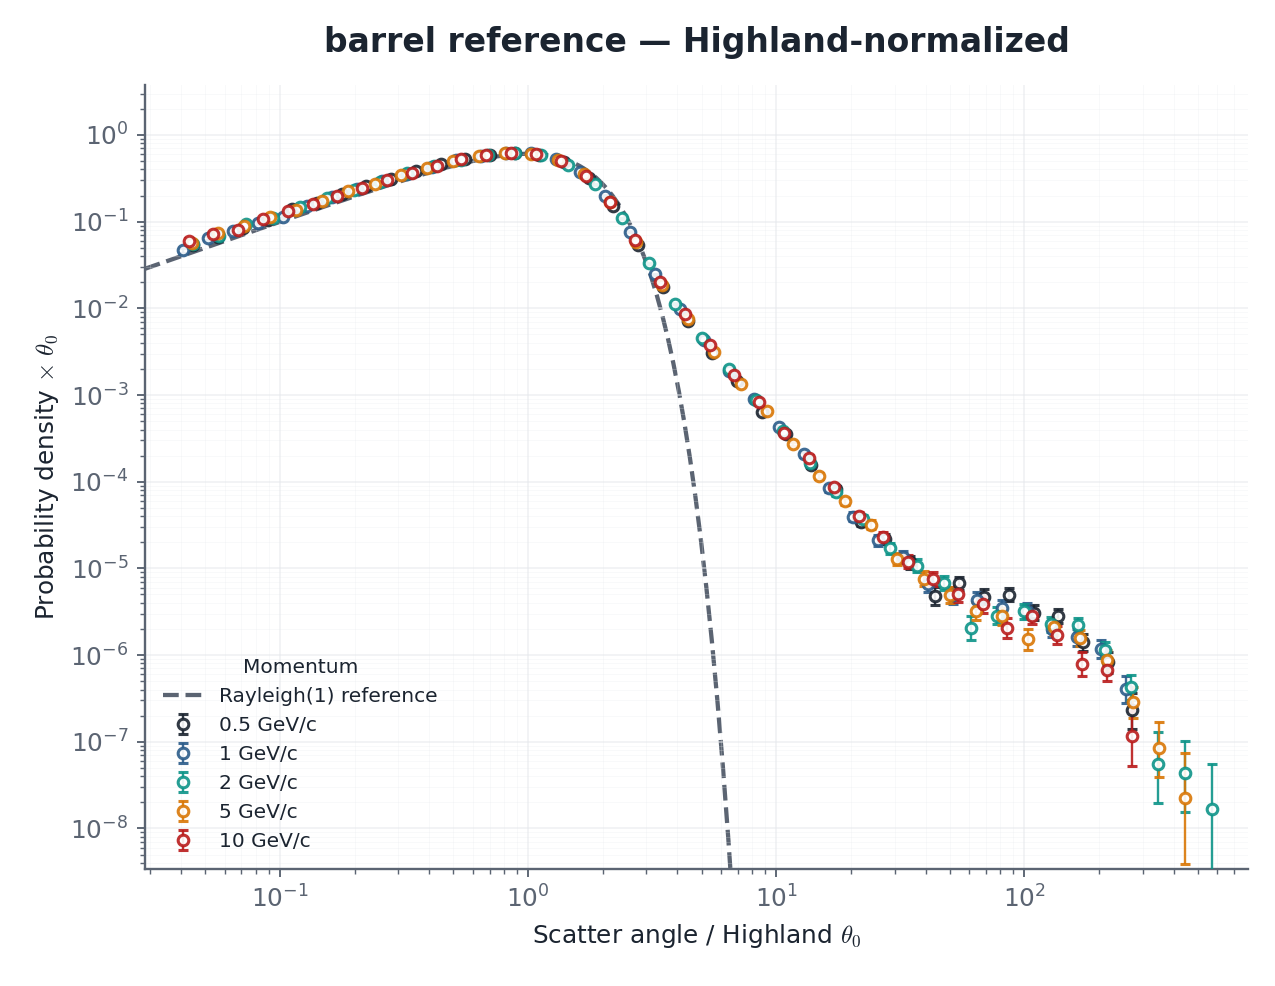
\includegraphics[width=\textwidth]{figures/fig_scattering_mixture_rescaled.png}
    \caption{Barrel-reference data rescaled by each momentum's own Highland $\theta_0$, collapsing all five momenta onto a single curve; dashed line is the Rayleigh(1) reference core shape}
    \label{fig:mixture_b}
\end{subfigure}

\vspace{0.4em}
\begin{subfigure}[b]{0.32\textwidth}
    \centering
    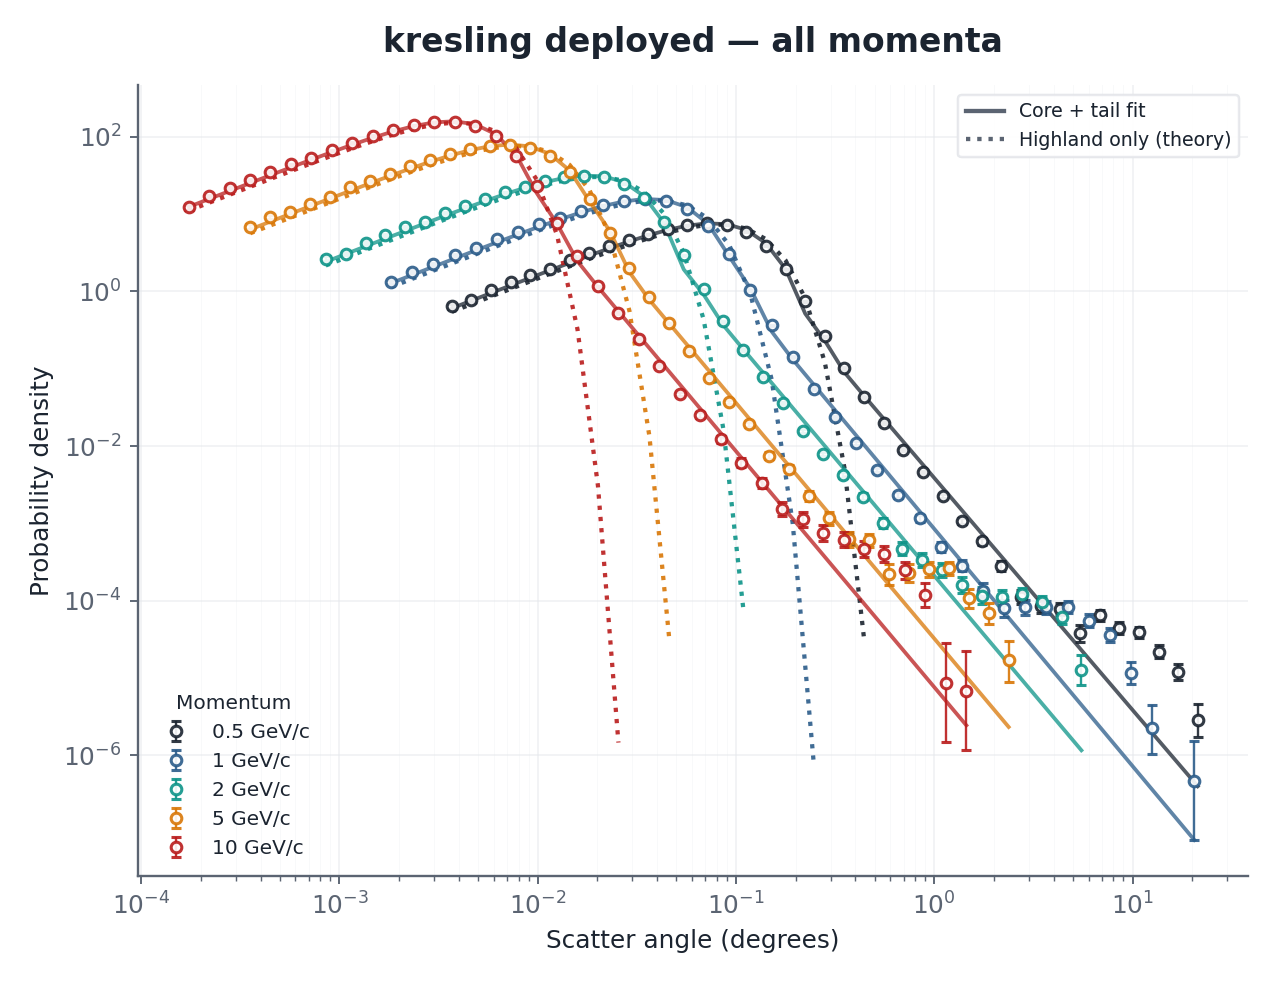
\includegraphics[width=\textwidth]{figures/fig_scattering_mixture_kresling.png}
    \caption{Kresling, all momenta}
    \label{fig:mixture_c}
\end{subfigure}
\hfill
\begin{subfigure}[b]{0.32\textwidth}
    \centering
    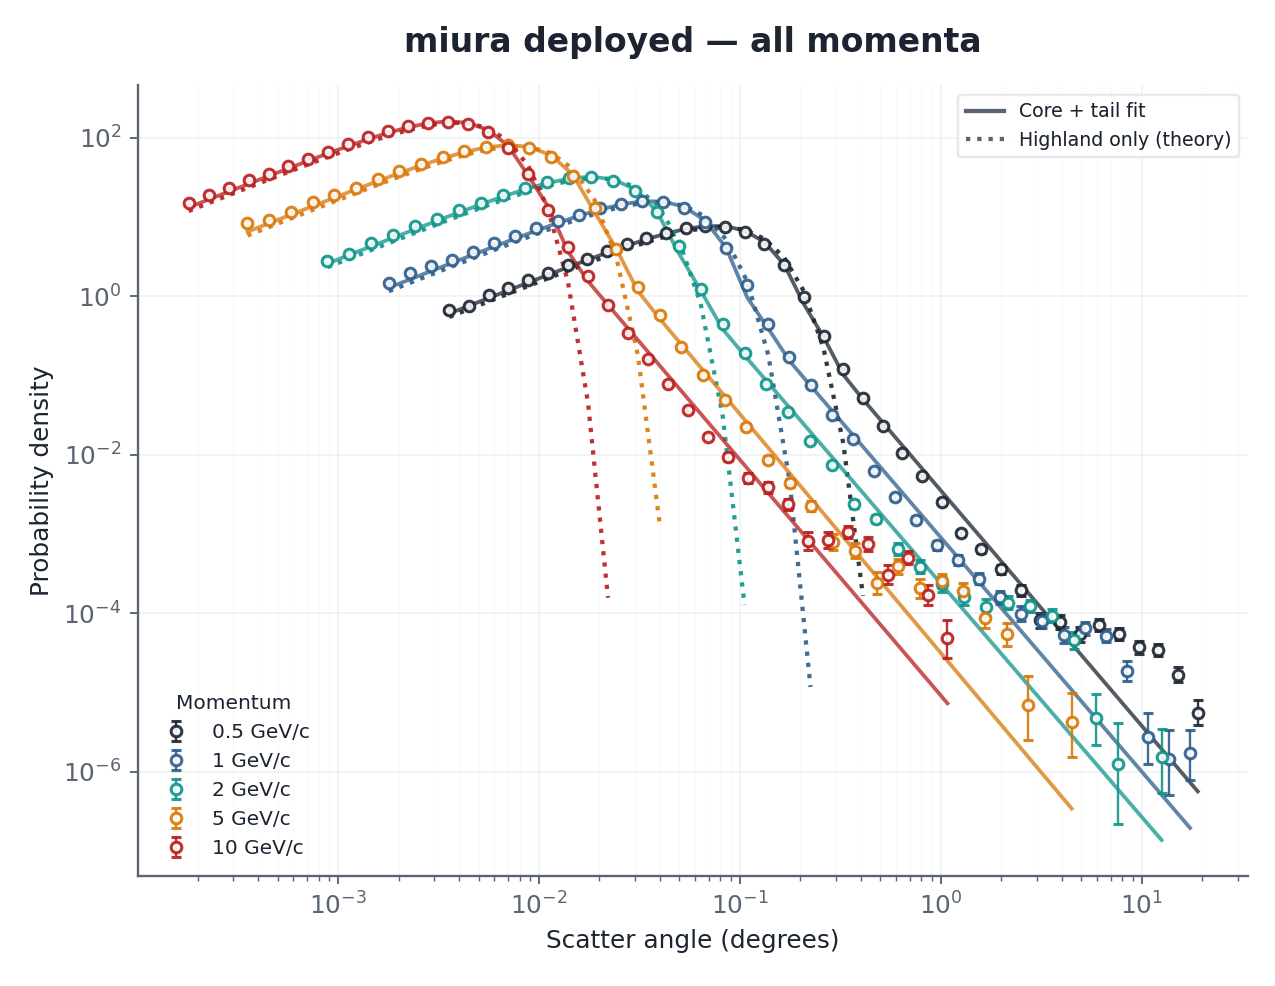
\includegraphics[width=\textwidth]{figures/fig_scattering_mixture_miura.png}
    \caption{Miura-ori, all momenta}
    \label{fig:mixture_d}
\end{subfigure}
\hfill
\begin{subfigure}[b]{0.32\textwidth}
    \centering
    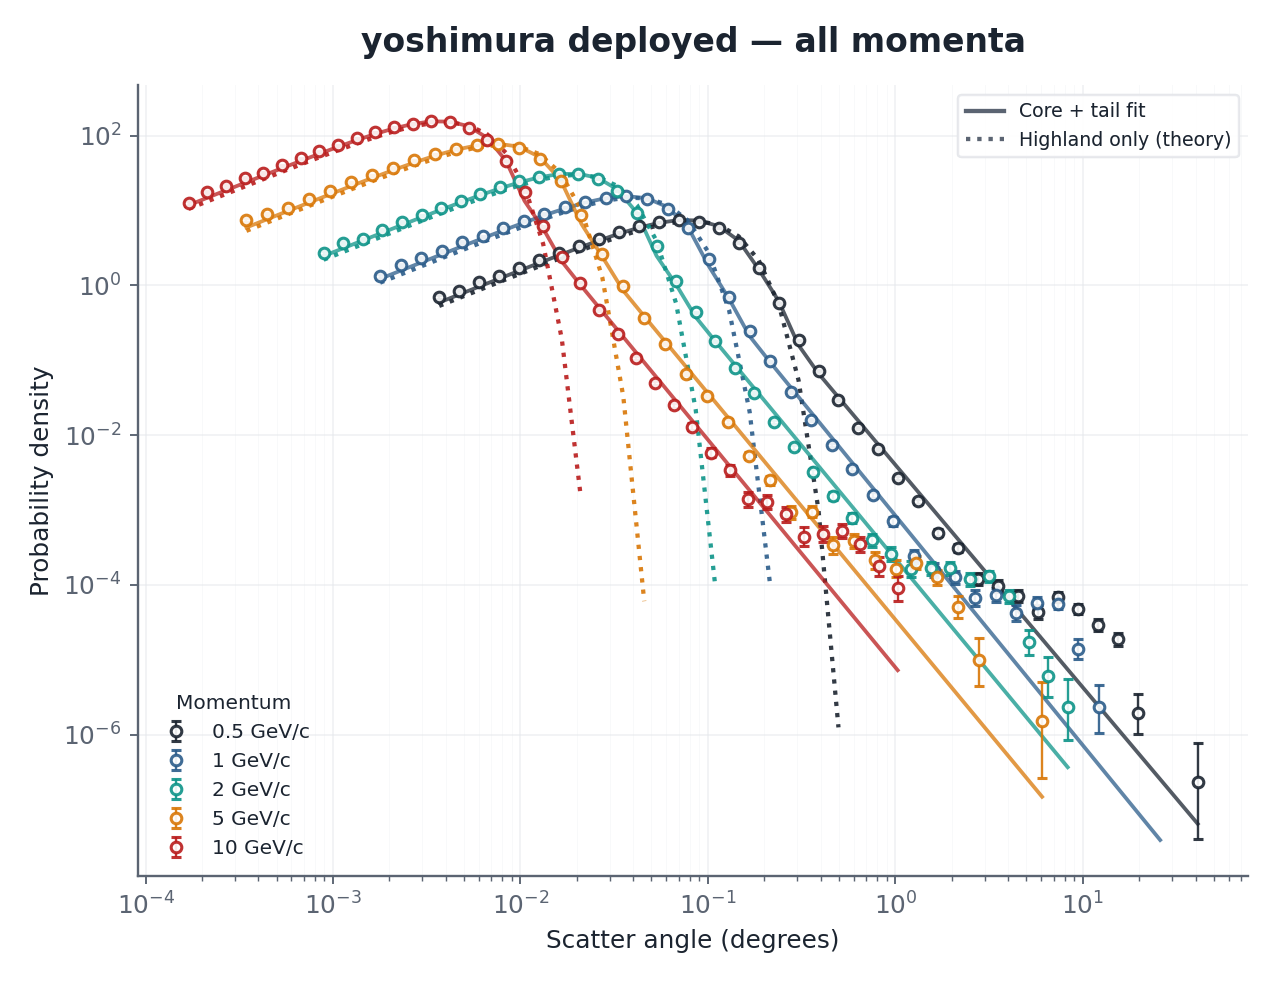
\includegraphics[width=\textwidth]{figures/fig_scattering_mixture_yoshimura.png}
    \caption{Yoshimura, all momenta}
    \label{fig:mixture_e}
\end{subfigure}

\caption{Multiple-scattering validation, Rayleigh-core-plus-Rutherford-tail mixture fit for the barrel reference and candidate fold geometries across all five simulated momenta (0.5--10~GeV/$c$).}
\label{fig:scattering_mixture}
\end{figure}

\begin{figure}[!htbp]
\centering
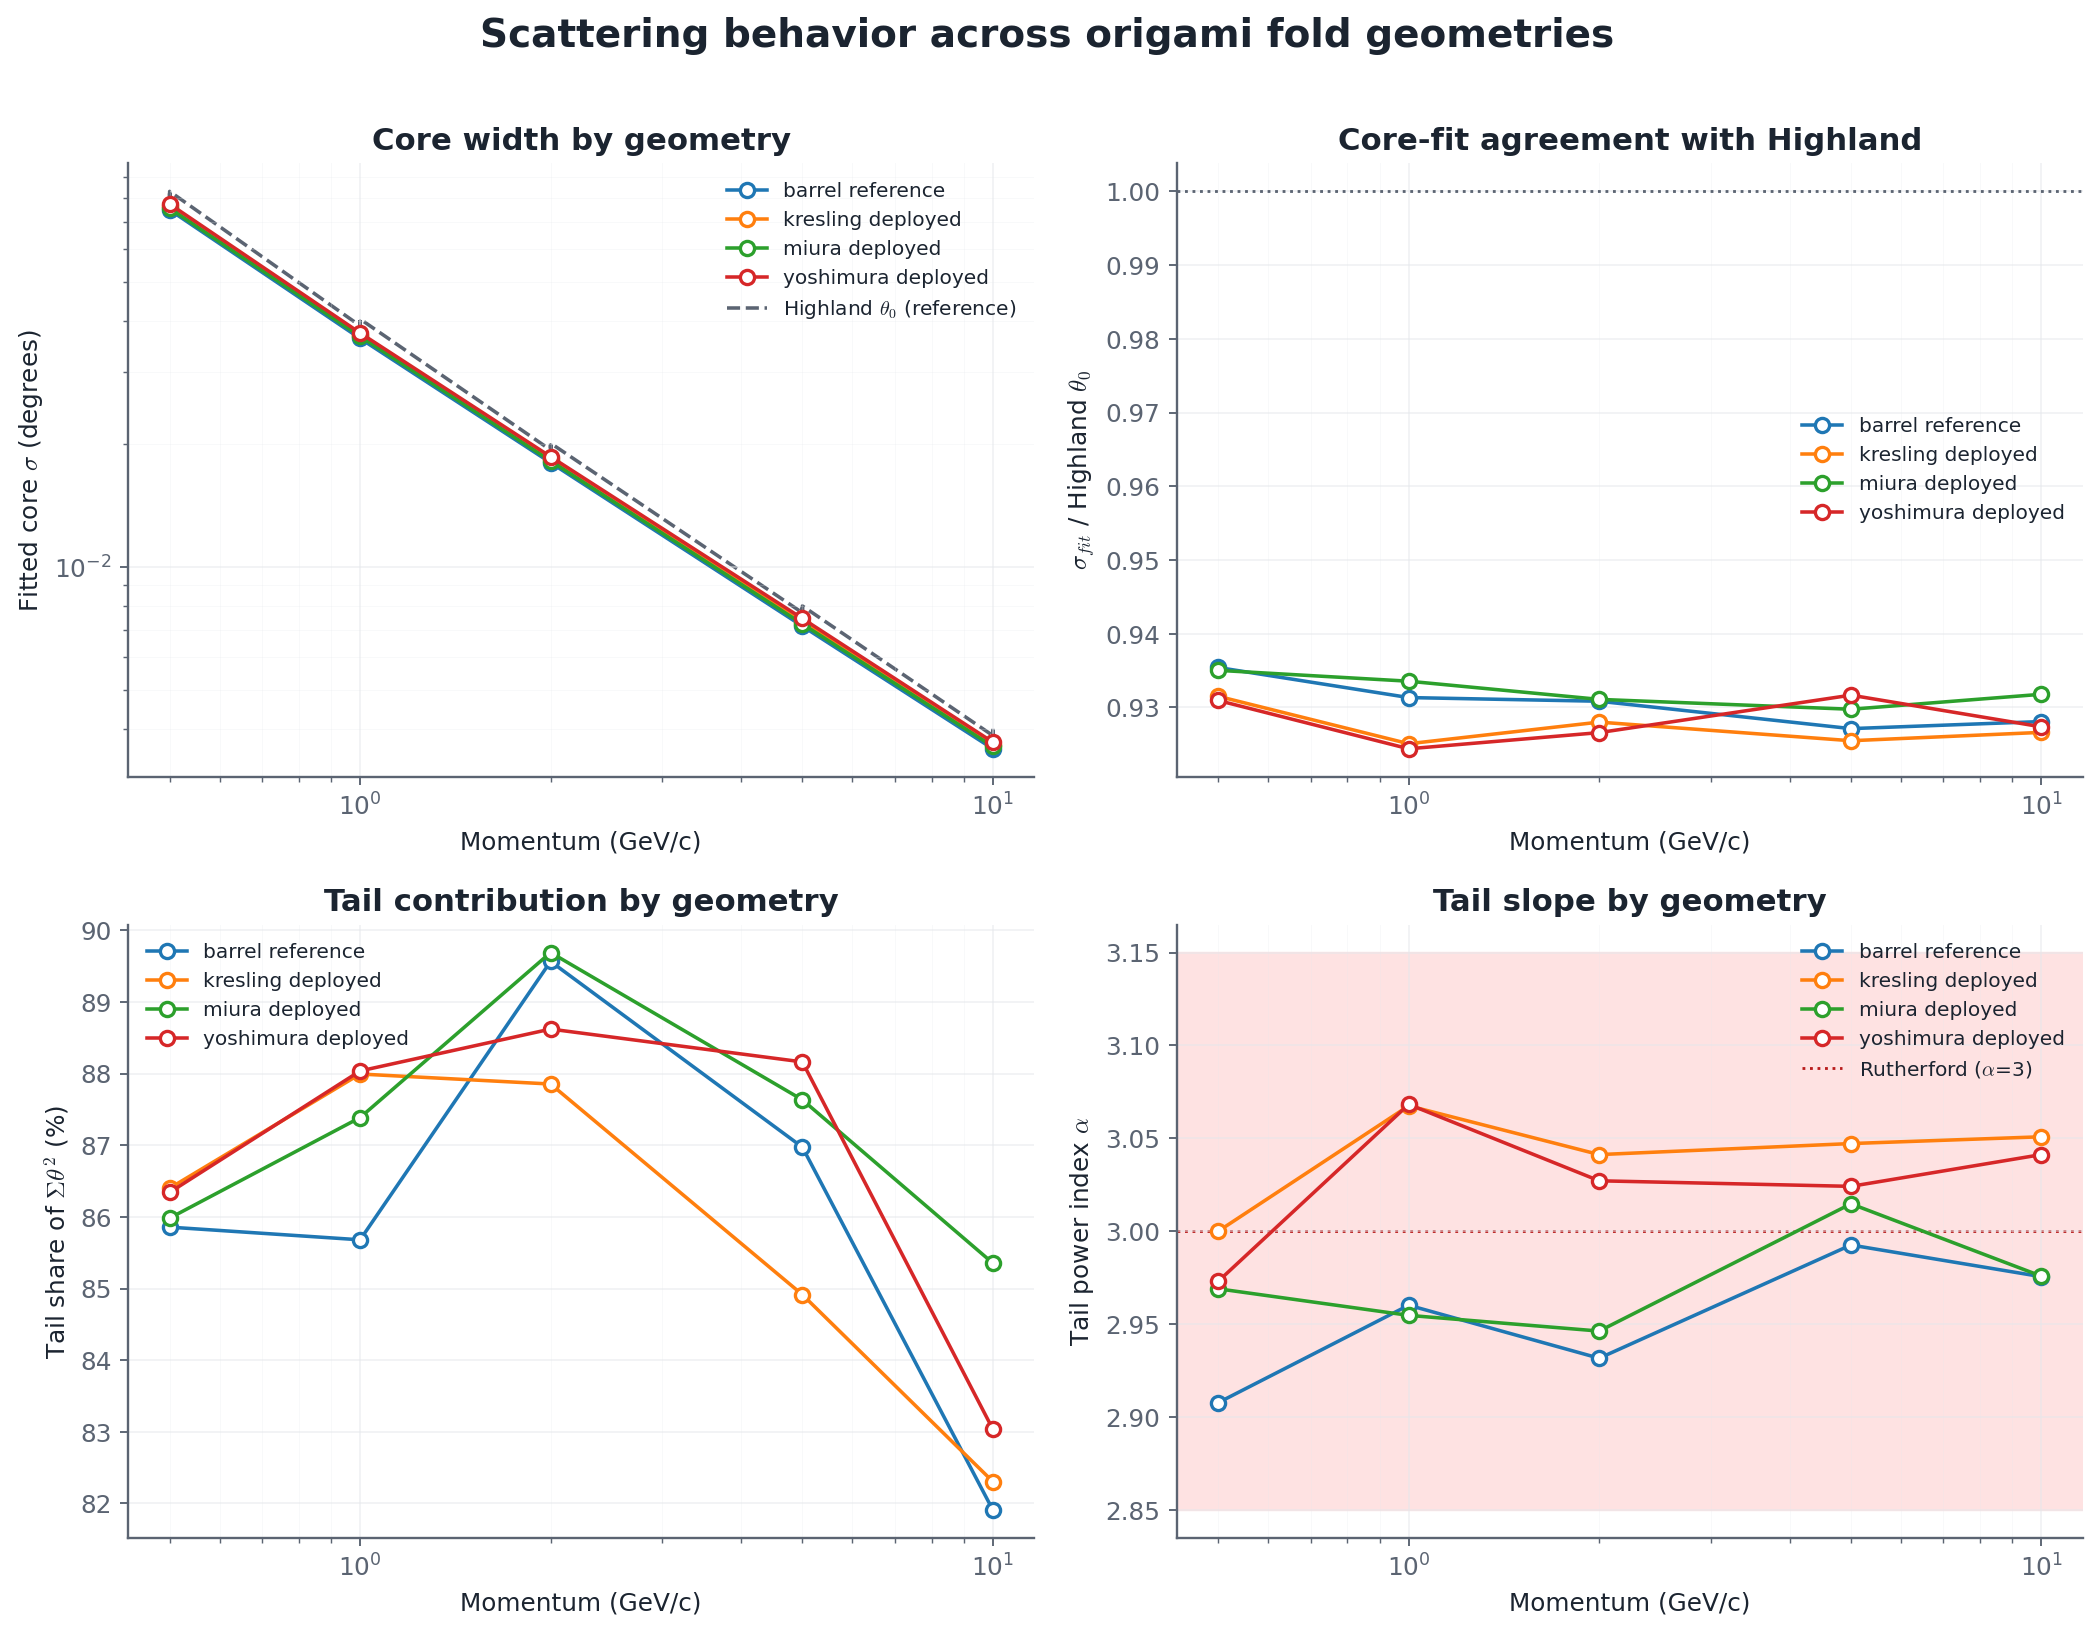
\includegraphics[width=0.92\textwidth]{figures/fig_scattering_mixture_summary.png}
\caption{Summary of multiple-scattering mixture fit across all four geometries and all five momenta: fitted core width vs.\ Highland $\theta_0$ (top left), core-fit/Highland ratio (top right, 0.924--0.935 across the full dataset), tail's share of total $\sum\theta^2$ (bottom left, 82--90\% throughout), and fitted tail power index $\alpha$ (bottom right, clustering at the Rutherford-predicted value of 3 across every geometry and momentum).}
\label{fig:scattering_mixture_summary}
\label{fig:mixture_f}
\end{figure}
\FloatBarrier
% NOTE: Table~\ref{tab:highland_mixture_fits} (full 20-row per-configuration fit results,
% referenced above) belongs in Appendix~\ref{sec:appendix_highland}, not in this section.
% Add it there, not here.

\section{Related Work}
\label{sec:related}

There are three main areas of previous work that are related to this project: curved and tilted silicon detectors, origami-based foldable structures, and radiation-length calculations. These areas give the main ideas behind this project, but none of them directly studies the folded detector shapes used here.

\subsection{Curved and tilted silicon tracking detectors}

The idea of using non-flat detector layers is already being studied in some high-energy physics experiments. One important example is the ALICE ITS3 detector. It uses very thin CMOS silicon sensors that can be bent into a cylindrical shape. The sensors can be bent to radii of $18$, $24$, and $30\text{ mm}$, while keeping the material budget at around $0.05\%\ X_0$ per layer~\cite{ALICE2024, Sonneveld2023}. Since the sensors are curved, there are no tile joints between separate flat sensors. However, this requires the silicon to be extremely thin and flexible enough to bend without being damaged.

The approach in this project is different. Instead of bending the silicon, the detector is made using flat sections connected by fold lines. This allows the overall detector to have a curved or non-planar shape while keeping the silicon itself flat.

Another useful example is the LHCb Upstream Tracker. It uses normal silicon sensor tiles together with flexible Kapton circuit boards. The Kapton is mainly used for electrical connections, signal routing, and power distribution~\cite{Lionetto2014}. The detector stack used in this project is also based on silicon sensors attached to a flexible substrate. However, here the flexible substrate has an additional purpose: it also helps the detector change its overall shape.

The CMS Phase-2 Outer Tracker uses another method. Its detector modules are tilted at different angles along the $z$-axis. This helps reduce dead areas and improves the detection of tracks, especially for tracks at high pseudorapidity~\cite{CMS2017}. This is different from the folding method used in this project because the CMS modules are still flat and are simply placed at different angles.

As far as the author knows, these existing detector projects have not directly compared origami-style folded detector geometries with a tiled detector of the same radius using full particle-transport simulation. This is the main area that this project tries to study.

\subsection{Origami fold patterns as deployable structures}

The fold patterns used in this project are based on existing ideas from origami and deployable structures. These patterns were originally developed for applications such as space structures and thin shells, rather than particle detectors.

Miura-ori is a well-known origami pattern that was developed for folding and deploying large sheets and membranes~\cite{Miura1985}. One of its main advantages is that the sheet can change from a flat shape to a folded or deployed shape while the individual sections remain mostly rigid. This makes it useful when a large change in shape is needed without bending the whole material.

The Yoshimura pattern comes from the study of thin cylindrical shells under compression. It has a diamond-like folding pattern and was later used as a deliberate folding structure~\cite{Yoshimura1955}. Kresling is another fold pattern that produces both rotation and shortening when it is compressed. It can also have different stable folded and deployed states~\cite{Kresling2008}.

These origami patterns are therefore not new. The new part of this project is using them for a detector and checking whether they can provide good hit acceptance while keeping the amount of material crossed by particles reasonably low.

\subsection{Radiation Length and Material-Budget Simulation}

Radiation length is a central figure of merit for particle tracking detectors. For a planar layer of thickness $t$, the material traversed at normal incidence is given by
\begin{equation}
\frac{X}{X_0} = \frac{t}{X_0}\,.
\end{equation}
For a track traversing the sensor at a local incidence angle $\theta_{\mathrm{local}}$, the geometric path length increases as
\begin{equation}
t_{\mathrm{path}} = \frac{t}{\cos\theta_{\mathrm{local}}}\,.
\end{equation}
These analytical relations provide the benchmark against which the simulation's step-level material accumulator is validated.

\textsc{Geant4}~\cite{Agostinelli2003} is employed to model particle transport, ionization energy loss, multiple Coulomb scattering, and secondary particle production. By maintaining identical sensor and substrate material definitions across all candidate designs, the simulation isolates the geometric consequences of fold topology from material composition effects.

\FloatBarrier
\section{Results}
\label{sec:results}

\subsection{Barrel Tile-Count Sensitivity and Headline Performance}
\label{sec:headline_results}

Before evaluating candidate geometries, the sensitivity of the barrel baseline to tile faceting ($N_{\text{cols}}$) was examined. An inscribed $n$-sided polygon of radius $R$ exhibits a geometric sagitta $s = R(1 - \cos(\pi/n))$. Coarse faceting ($N_{\text{cols}} = 24$, $s = 0.342\text{ mm}$) increases the mean local incidence angle by $1.70^\circ$ relative to fine faceting ($N_{\text{cols}} = 141$, $s = 0.0099\text{ mm}$), shifting acceptance by $+0.512$ pp and mean path length by $+1.54\%$ ($z \approx 6.9$, Table~\ref{tab:barrel_sensitivity}). The fine-tiled barrel ($N_{\text{cols}} = 141$) is therefore used as the reference baseline throughout all subsequent evaluations.

\begin{table}[!htbp]
\centering
\caption{Barrel baseline sensitivity to tile faceting ($500{,}000$ primary pions, $R = 40\text{ mm}$, scored under material-differentiated radiation lengths).}
\label{tab:barrel_sensitivity}
\smallskip
\resizebox{0.85\textwidth}{!}{
\begin{tabular}{lcccc}
\toprule
Configuration & Hits / Total & Acceptance & Mean Path ($X_0$) & $\langle\theta_{\text{local}}\rangle$ \\
\midrule
Barrel (coarse, 24 cols) & 418,388 / 500,000 & 0.836776 & $0.0040378 \pm 1.17\times 10^{-6}$ & $27.97^\circ$ \\
Barrel (fine, 141 cols)   & 415,828 / 500,000 & 0.831656 & $0.0039765 \pm 1.14\times 10^{-6}$ & $26.27^\circ$ \\
\bottomrule
\end{tabular}
}
\end{table}

Headline single-run performance metrics at nominal $300\ \mu\text{m}$ silicon are reported in Table~\ref{tab:headline_results}.

\begin{table}[!htbp]
\centering
\caption{Single-run exploratory performance metrics for candidate geometries ($500{,}000$ primaries each). Multi-run replication ground-truth means and uncertainties are reported in Table~\ref{tab:multirun_results}.}
\label{tab:headline_results}
\smallskip
\resizebox{\textwidth}{!}{
\begin{tabular}{lcccccc}
\toprule
Geometry & Hits / Total & Acceptance & Mean $X/X_0$ & 95\% CI & Median $X/X_0$ & IQR \\
\midrule
Barrel (fine) & 415,828 / 500,000 & 0.831656 & 0.003977 & [0.003973, 0.003980] & 0.003661 & 0.000854 \\
Miura-ori     & 418,227 / 500,000 & 0.836454 & 0.004051 & [0.004048, 0.004055] & 0.003737 & 0.000869 \\
Kresling      & 427,617 / 500,000 & 0.855234 & 0.004203 & [0.004199, 0.004207] & 0.003884 & 0.000908 \\
Yoshimura     & 422,427 / 500,000 & 0.844854 & 0.004295 & [0.004291, 0.004299] & 0.003950 & 0.000932 \\
\bottomrule
\end{tabular}
}
\end{table}

Pairwise comparisons across the 5-run replications (Table~\ref{tab:pairwise_tests}) confirm that Kresling achieves the highest overall acceptance ($+2.362$ pp over barrel, $95\%$ CI $[+2.326, +2.398]$ pp, Cohen's $h = +0.065$), followed by Yoshimura ($+1.304$ pp, $95\%$ CI $[+1.249, +1.358]$ pp, Cohen's $h = +0.035$) and Miura-ori ($+0.493$ pp, $95\%$ CI $[+0.452, +0.535]$ pp, Cohen's $h = +0.013$). In material cost, Yoshimura incurs the largest penalty ($+8.01\%$ in $X_0$ over barrel), exceeding Kresling ($+5.69\%$) and Miura-ori ($+1.88\%$).

\begin{table}[!htbp]
\centering
\caption{Pairwise acceptance comparisons across 5-run replications, reporting mean acceptance difference ($\Delta A$), 95\% confidence intervals, standardized effect size (Cohen's $h$), and Holm--Bonferroni corrected significance.}
\label{tab:pairwise_tests}
\smallskip
\resizebox{0.95\textwidth}{!}{
\begin{tabular}{lcccc}
\toprule
Pairwise comparison & $\Delta A$ (pp) & 95\% CI (pp) & Cohen's $h$ & Significant? ($p < 10^{-7}$) \\
\midrule
Barrel (fine) vs.\ Kresling   & $+2.362$ & $[+2.326, +2.398]$ & $+0.065$ & Yes \\
Miura-ori vs.\ Kresling        & $+1.868$ & $[+1.838, +1.899]$ & $+0.052$ & Yes \\
Barrel (fine) vs.\ Yoshimura  & $+1.304$ & $[+1.249, +1.358]$ & $+0.035$ & Yes \\
Kresling vs.\ Yoshimura        & $-1.058$ & $[-1.104, -1.012]$ & $-0.030$ & Yes \\
Miura-ori vs.\ Yoshimura       & $+0.810$ & $[+0.759, +0.861]$ & $+0.022$ & Yes \\
Barrel (fine) vs.\ Miura-ori  & $+0.493$ & $[+0.452, +0.535]$ & $+0.013$ & Yes \\
\bottomrule
\end{tabular}
}
\end{table}

The run-to-run standard deviations ($\text{SD}_A \le 0.05$ pp, Table~\ref{tab:multirun_results}) across five independent runs per geometry are an order of magnitude smaller than the inter-geometry acceptance differences, confirming high physical reproducibility.

\begin{table}[!htbp]
\centering
\caption{Five-run replication summary (Mean $\pm$ SD and SEM, $5 \times 500{,}000$ primaries).}
\label{tab:multirun_results}
\smallskip
\begin{tabular}{lcccccc}
\toprule
Geometry & Mean $A$ & $\text{SD}_A$ & $\text{SEM}_A$ & Mean $X_0$ & $\text{SD}_{X0}$ & $\text{SEM}_{X0}$ \\
\midrule
Barrel (fine) & 0.831784 & 0.000366 & 0.000164 & 0.0039765 & $5.36\times 10^{-7}$ & $2.40\times 10^{-7}$ \\
Miura-ori     & 0.836718 & 0.000296 & 0.000132 & 0.0040514 & $1.13\times 10^{-6}$ & $5.07\times 10^{-7}$ \\
Kresling      & 0.855400 & 0.000184 & 0.000082 & 0.0042029 & $1.66\times 10^{-6}$ & $7.40\times 10^{-7}$ \\
Yoshimura     & 0.844820 & 0.000497 & 0.000222 & 0.0042950 & $4.77\times 10^{-7}$ & $2.13\times 10^{-7}$ \\
\bottomrule
\end{tabular}
\end{table}

\FloatBarrier
\subsection{Circumferential Facet-Count (\texorpdfstring{$N$}{N}) Sweep and Geometric Singularities}
\label{sec:n_sweep}

Sweeping facet count $N \in \{6, 8, 12, 16, 24, 32\}$ reveals fundamental convergence trends (Table~\ref{tab:n_sweep} and Figure~\ref{fig:n_sweep}). For all three families, acceptance gains asymptotically converge toward the smooth barrel limit as $N$ increases (Kresling drops from $+2.31$ pp at $N=6$ to $-0.00$ pp at $N=32$).

\begin{figure}[!htbp]
\centering
\begin{subfigure}[b]{0.45\textwidth}
    \centering
    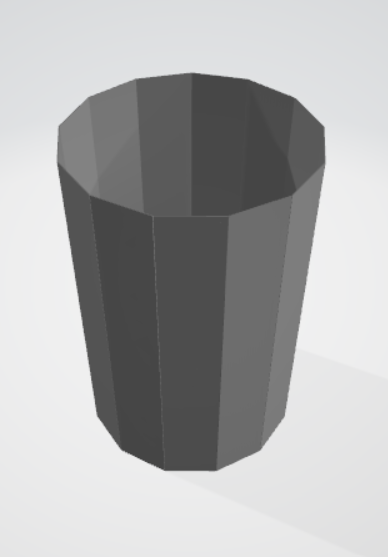
\includegraphics[width=\textwidth]{figures/fig3_yoshimura_degenerate_n6.png}
    \caption{Degenerate Kresling ($N=12$, $\theta_{\text{twist}} = 30^\circ$)}
    \label{fig:kresling_deg}
\end{subfigure}
\hfill
\begin{subfigure}[b]{0.45\textwidth}
    \centering
    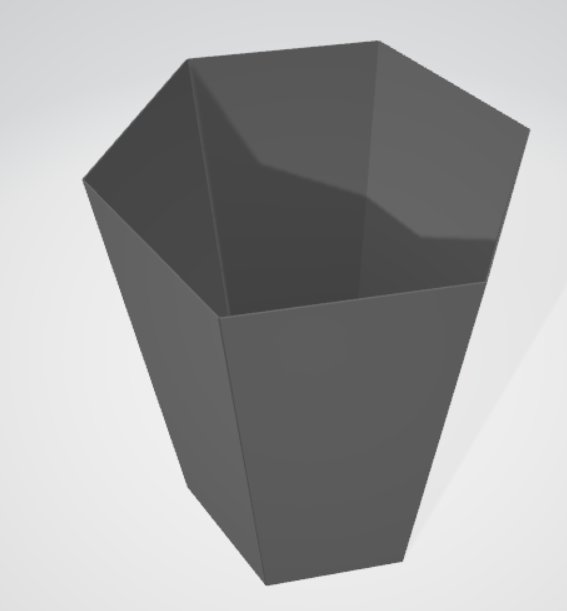
\includegraphics[width=\textwidth]{figures/fig_kresling_degenerate.png}
    \caption{Degenerate Yoshimura ($N=6$, $\theta = 30^\circ$)}
    \label{fig:yoshi_deg}
\end{subfigure}
\caption{Direct 3D renders of the excluded degenerate configurations resulting from closed-form rotational periodicity cancellation: (a) Kresling $N=12$ collapsing to an untwisted faceted cylinder, and (b) Yoshimura $N=6$ collapsing to a plain tapered hexagonal frustum.}
\label{fig:degenerate_renders}
\end{figure}

\begin{table}[!htbp]
\centering
\caption{Facet-count ($N$) sweep differences relative to the fine barrel reference.}
\label{tab:n_sweep}
\smallskip
\resizebox{\textwidth}{!}{
\begin{tabular}{rcccccc}
\toprule
$N$ & Kresling $\Delta A$ & Kresling $\Delta X_0$ & Miura $\Delta A$ & Miura $\Delta X_0$ & Yoshi $\Delta A$ & Yoshi $\Delta X_0$ \\
\midrule
6  & $+2.31\text{ pp}$ & $+5.72\%$ & $+2.34\text{ pp}$ & $+14.91\%$ & --- (excl.) & --- (excl.) \\
8  & $+1.26\text{ pp}$ & $+2.49\%$ & $+1.39\text{ pp}$ & $+6.41\%$  & $+1.34\text{ pp}$ & $+8.03\%$ \\
12 & --- (excl.)        & --- (excl.)& $+0.56\text{ pp}$ & $+2.30\%$  & $+0.60\text{ pp}$ & $+13.24\%$ \\
16 & $+0.31\text{ pp}$ & $+1.70\%$ & $+0.41\text{ pp}$ & $+1.23\%$  & $+0.38\text{ pp}$ & $+18.39\%$ \\
24 & $+0.09\text{ pp}$ & $+2.26\%$ & $+0.17\text{ pp}$ & $+0.56\%$  & $+0.17\text{ pp}$ & $+29.53\%$ \\
32 & $-0.00\text{ pp}$ & $+2.57\%$ & $+0.13\text{ pp}$ & $+0.31\%$  & $+0.14\text{ pp}$ & $+41.78\%$ \\
\bottomrule
\end{tabular}
}
\end{table}

\begin{figure}[!htbp]
\centering
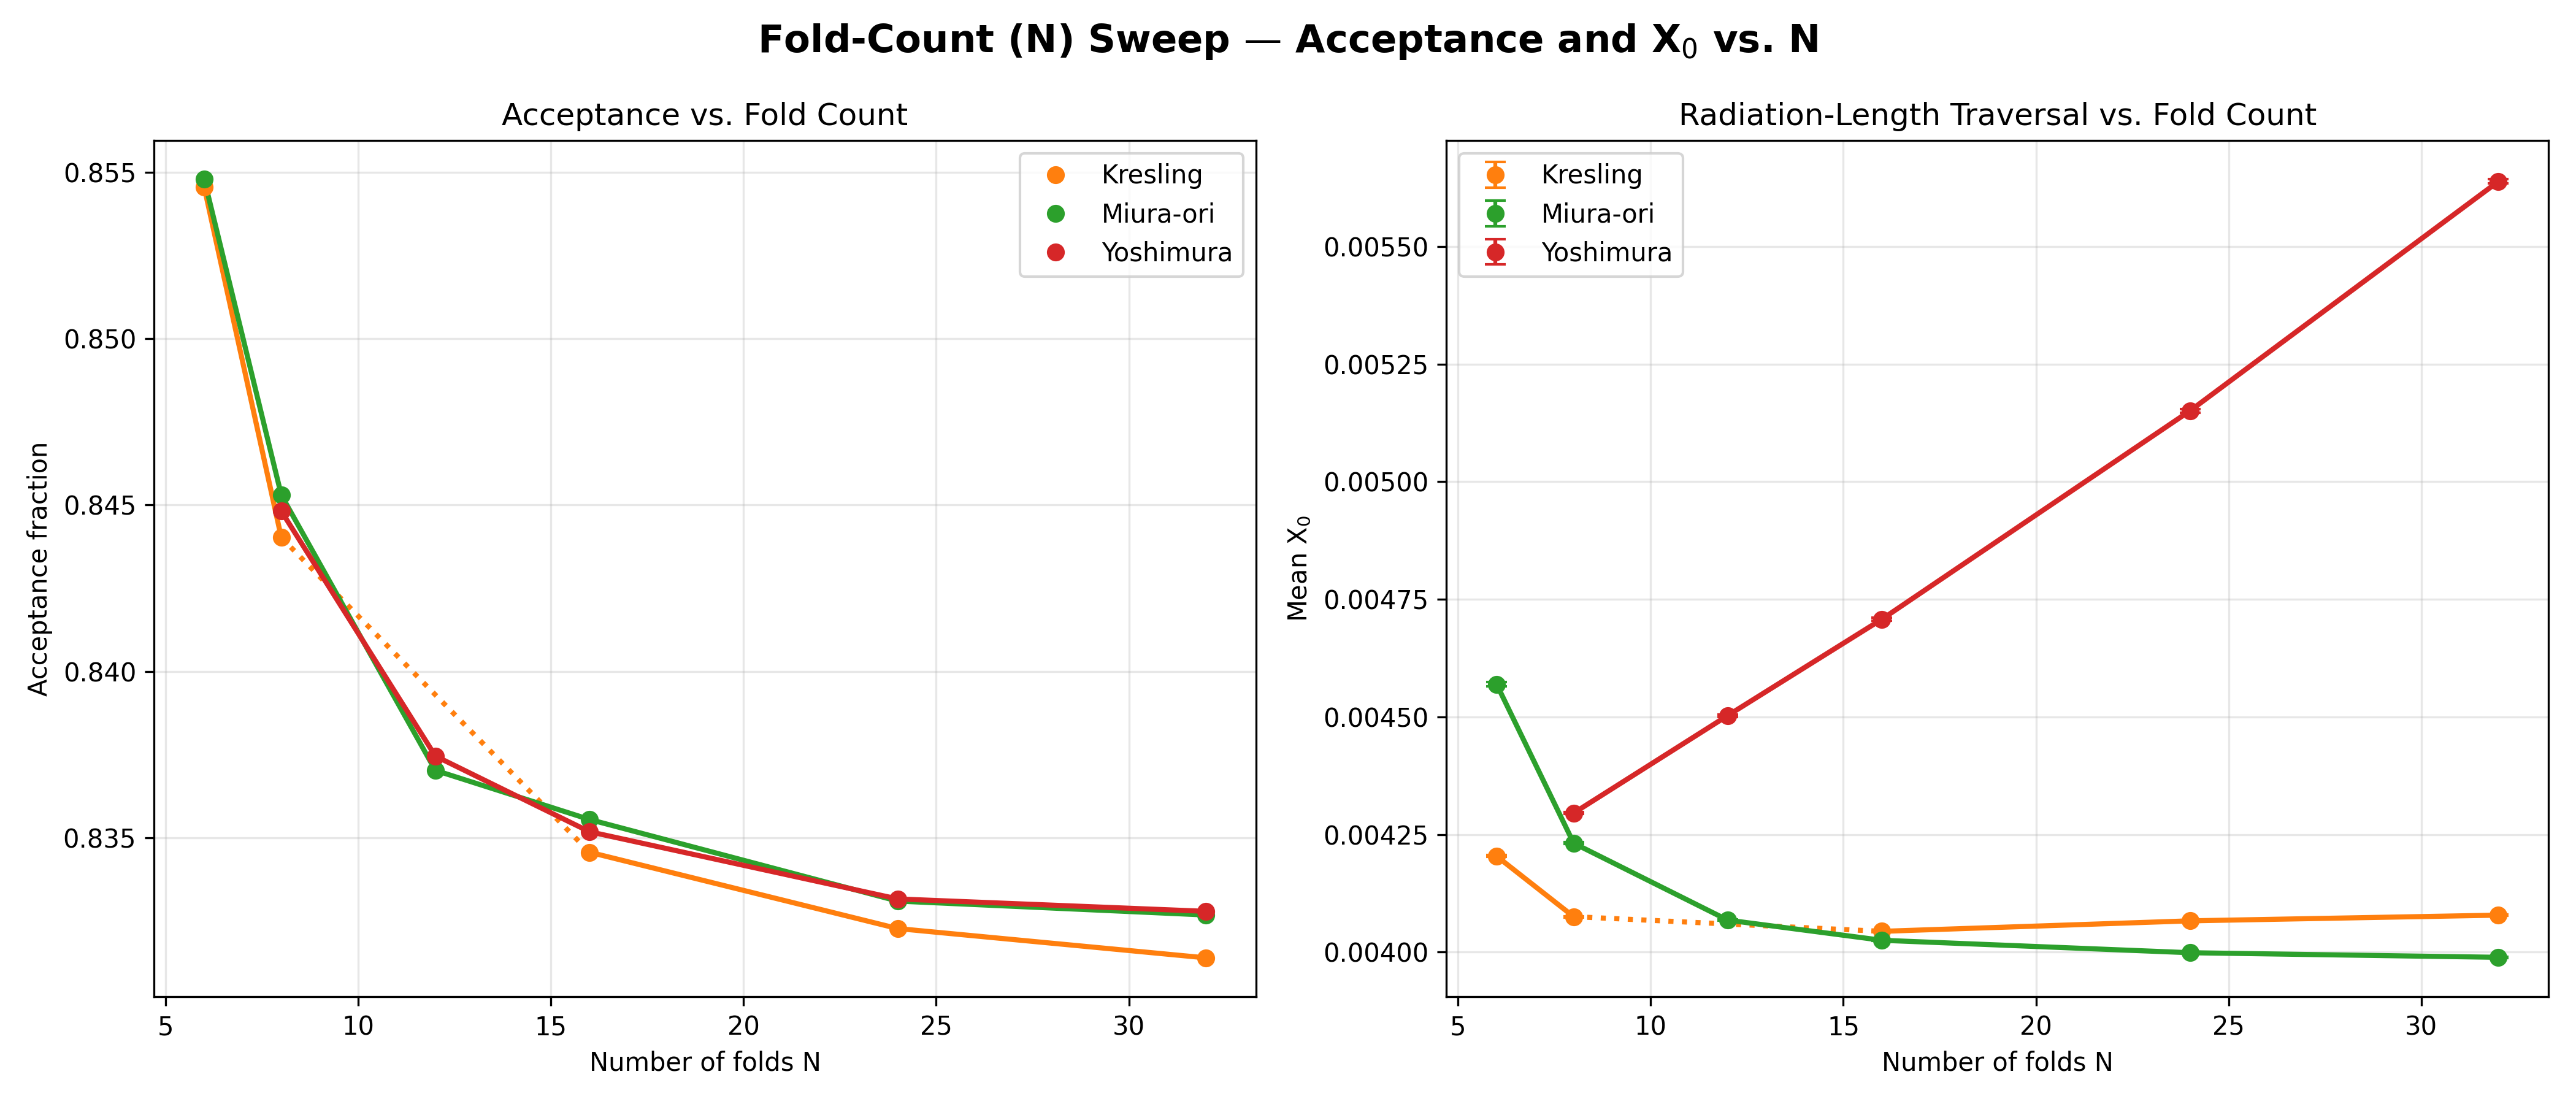
\includegraphics[width=0.90\textwidth]{figures/fig4_n_sweep.png}
\caption{Acceptance fraction gain $\Delta A$ (left) and mean radiation-length traversal excess $\Delta X_0$ (right) as a function of circumferential facet count $N$ across candidate fold families relative to the fine-tiled barrel baseline.}
\label{fig:n_sweep}
\end{figure}

In contrast, radiation length diverges between families: Miura-ori exhibits a monotonically decreasing material excess with larger $N$ (falling to $+0.31\%$ at $N=32$), whereas Kresling plateaus into a narrow band between $+1.70\%$ and $+2.57\%$ for $N \ge 8$, after an initial $+5.72\%$ penalty at the smallest facet count ($N = 6$), and Yoshimura exhibits an escalating material penalty, surging from $+8.03\%$ at $N=8$ to $+41.78\%$ at $N=32$. The nominal Miura-ori configuration ($N=13$) utilizes an odd facet count to satisfy circumferential anti-symmetric herringbone seam closure, interpolating smoothly between the $N=12$ and $N=16$ swept points. Two singular configurations---Yoshimura $N=6$ ($\theta = \pi/N$) and Kresling $N=12$ ($\theta_{\text{twist}} = 360^\circ/N$)---collapse into untwisted prismatic polygons (Figure~\ref{fig:degenerate_renders}) and are formally excluded.

\FloatBarrier
\subsection{Fold-Angle (\texorpdfstring{$\theta$}{theta}) Sensitivity}
\label{sec:theta_sweep}

Varying the fold angle $\theta \in \{15^\circ, 30^\circ, 45^\circ, 60^\circ, 75^\circ\}$ illustrates contrasting geometric stability (Table~\ref{tab:theta_sweep} and Figure~\ref{fig:theta_sweep}). Miura-ori and Kresling remain virtually flat across the entire angular domain (acceptance varying by $< 0.15$ pp). Conversely, Yoshimura exhibits extreme non-linear growth: acceptance increases from $0.8448$ to $0.9415$ while mean $X_0$ triples from $0.004060$ to $0.013303\ X_0$, driven by steep facet inclination angles. Kresling $\theta = 60^\circ$ represents an exact rotational periodicity degeneracy and is excluded.

\begin{table}[!htbp]
\centering
\caption{Fold-angle ($\theta$) sweep performance across fold families ($500{,}000$ primaries each).}
\label{tab:theta_sweep}
\smallskip
\begin{tabular}{ccccccc}
\toprule
$\theta$ & Kresling $A$ & Kresling $X_0$ & Miura $A$ & Miura $X_0$ & Yoshi $A$ & Yoshi $X_0$ \\
\midrule
$15^\circ$ & 0.8546 & 0.004184 & 0.8367 & 0.004076 & 0.8448 & 0.004060 \\
$30^\circ$ & 0.8554 & 0.004201 & 0.8369 & 0.004065 & 0.8450 & 0.004295 \\
$45^\circ$ & 0.8547 & 0.004181 & 0.8373 & 0.004053 & 0.8552 & 0.005522 \\
$60^\circ$ & --- (excl.) & --- (excl.) & 0.8371 & 0.004039 & 0.8918 & 0.008369 \\
$75^\circ$ & 0.8554 & 0.004575 & 0.8362 & 0.004031 & 0.9415 & 0.013303 \\
\bottomrule
\end{tabular}
\end{table}

\begin{figure}[!htbp]
\centering
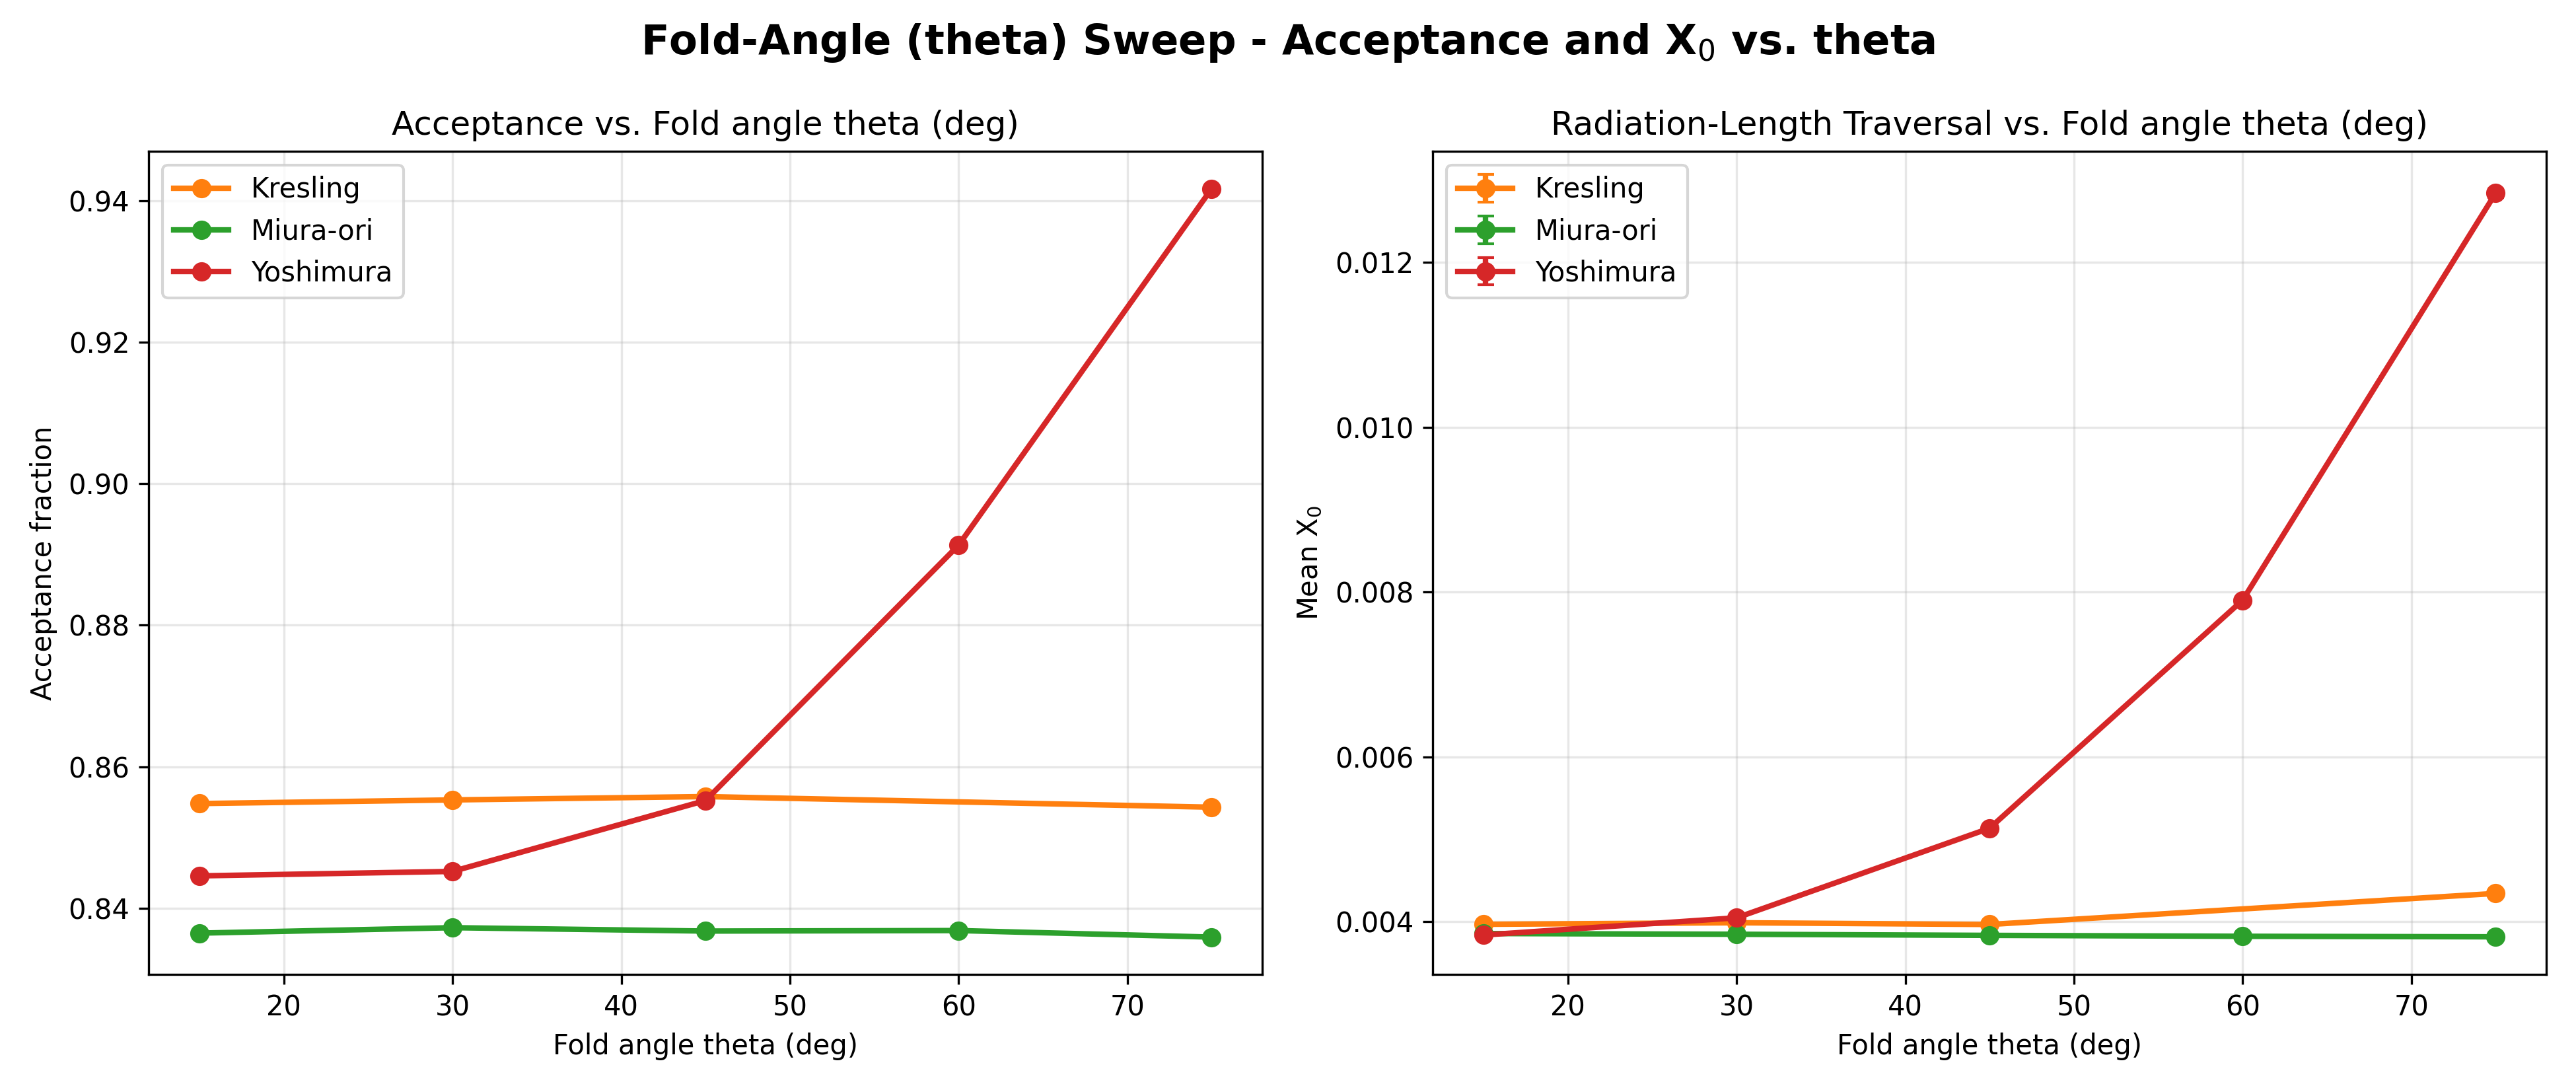
\includegraphics[width=0.90\textwidth]{figures/fig5_theta_sweep.png}
\caption{Acceptance fraction and mean radiation-length traversal $X_0$ versus fold angle $\theta$ across candidate fold families.}
\label{fig:theta_sweep}
\end{figure}

\FloatBarrier
\subsection{Vertex-Position Robustness}
\label{sec:vertex_robustness}

To confirm that the $3\text{ mm}$ vertex smear does not distort results, the Gaussian smear parameter was swept over $\sigma \in [0, 20]\text{ mm}$ alongside radial vertex displacement tests (Table~\ref{tab:vertex_smear} and Figure~\ref{fig:vertex_smear}). Performance is entirely stable up to $\sigma = 10\text{ mm}$ ($|\Delta A| < 0.2$ pp). At $\sigma = 20\text{ mm}$, the beam spot becomes comparable to the detector radius ($40\text{ mm}$), causing substantial off-center track leakage.

\begin{table}[!htbp]
\centering
\caption{Acceptance and mean $X_0$ as a function of 3D Gaussian vertex smear $\sigma$.}
\label{tab:vertex_smear}
\smallskip
\resizebox{\textwidth}{!}{
\begin{tabular}{rcccccccc}
\toprule
$\sigma$ (mm) & Barrel $A$ & Barrel $X_0$ & Kresling $A$ & Kresling $X_0$ & Miura $A$ & Miura $X_0$ & Yoshi $A$ & Yoshi $X_0$ \\
\midrule
0  & 0.8324 & 0.003962 & 0.8546 & 0.004185 & 0.8365 & 0.004035 & 0.8457 & 0.004274 \\
1  & 0.8317 & 0.003965 & 0.8545 & 0.004181 & 0.8371 & 0.004037 & 0.8447 & 0.004276 \\
5  & 0.8324 & 0.004004 & 0.8552 & 0.004241 & 0.8364 & 0.004084 & 0.8449 & 0.004334 \\
10 & 0.8315 & 0.004168 & 0.8546 & 0.004458 & 0.8355 & 0.004274 & 0.8439 & 0.004558 \\
20 & 0.7577 & 0.005341 & 0.7585 & 0.005888 & 0.7570 & 0.005576 & 0.7503 & 0.006002 \\
\bottomrule
\end{tabular}
}
\end{table}

\begin{figure}[!htbp]
\centering
\begin{subfigure}[b]{0.68\textwidth}
    \centering
    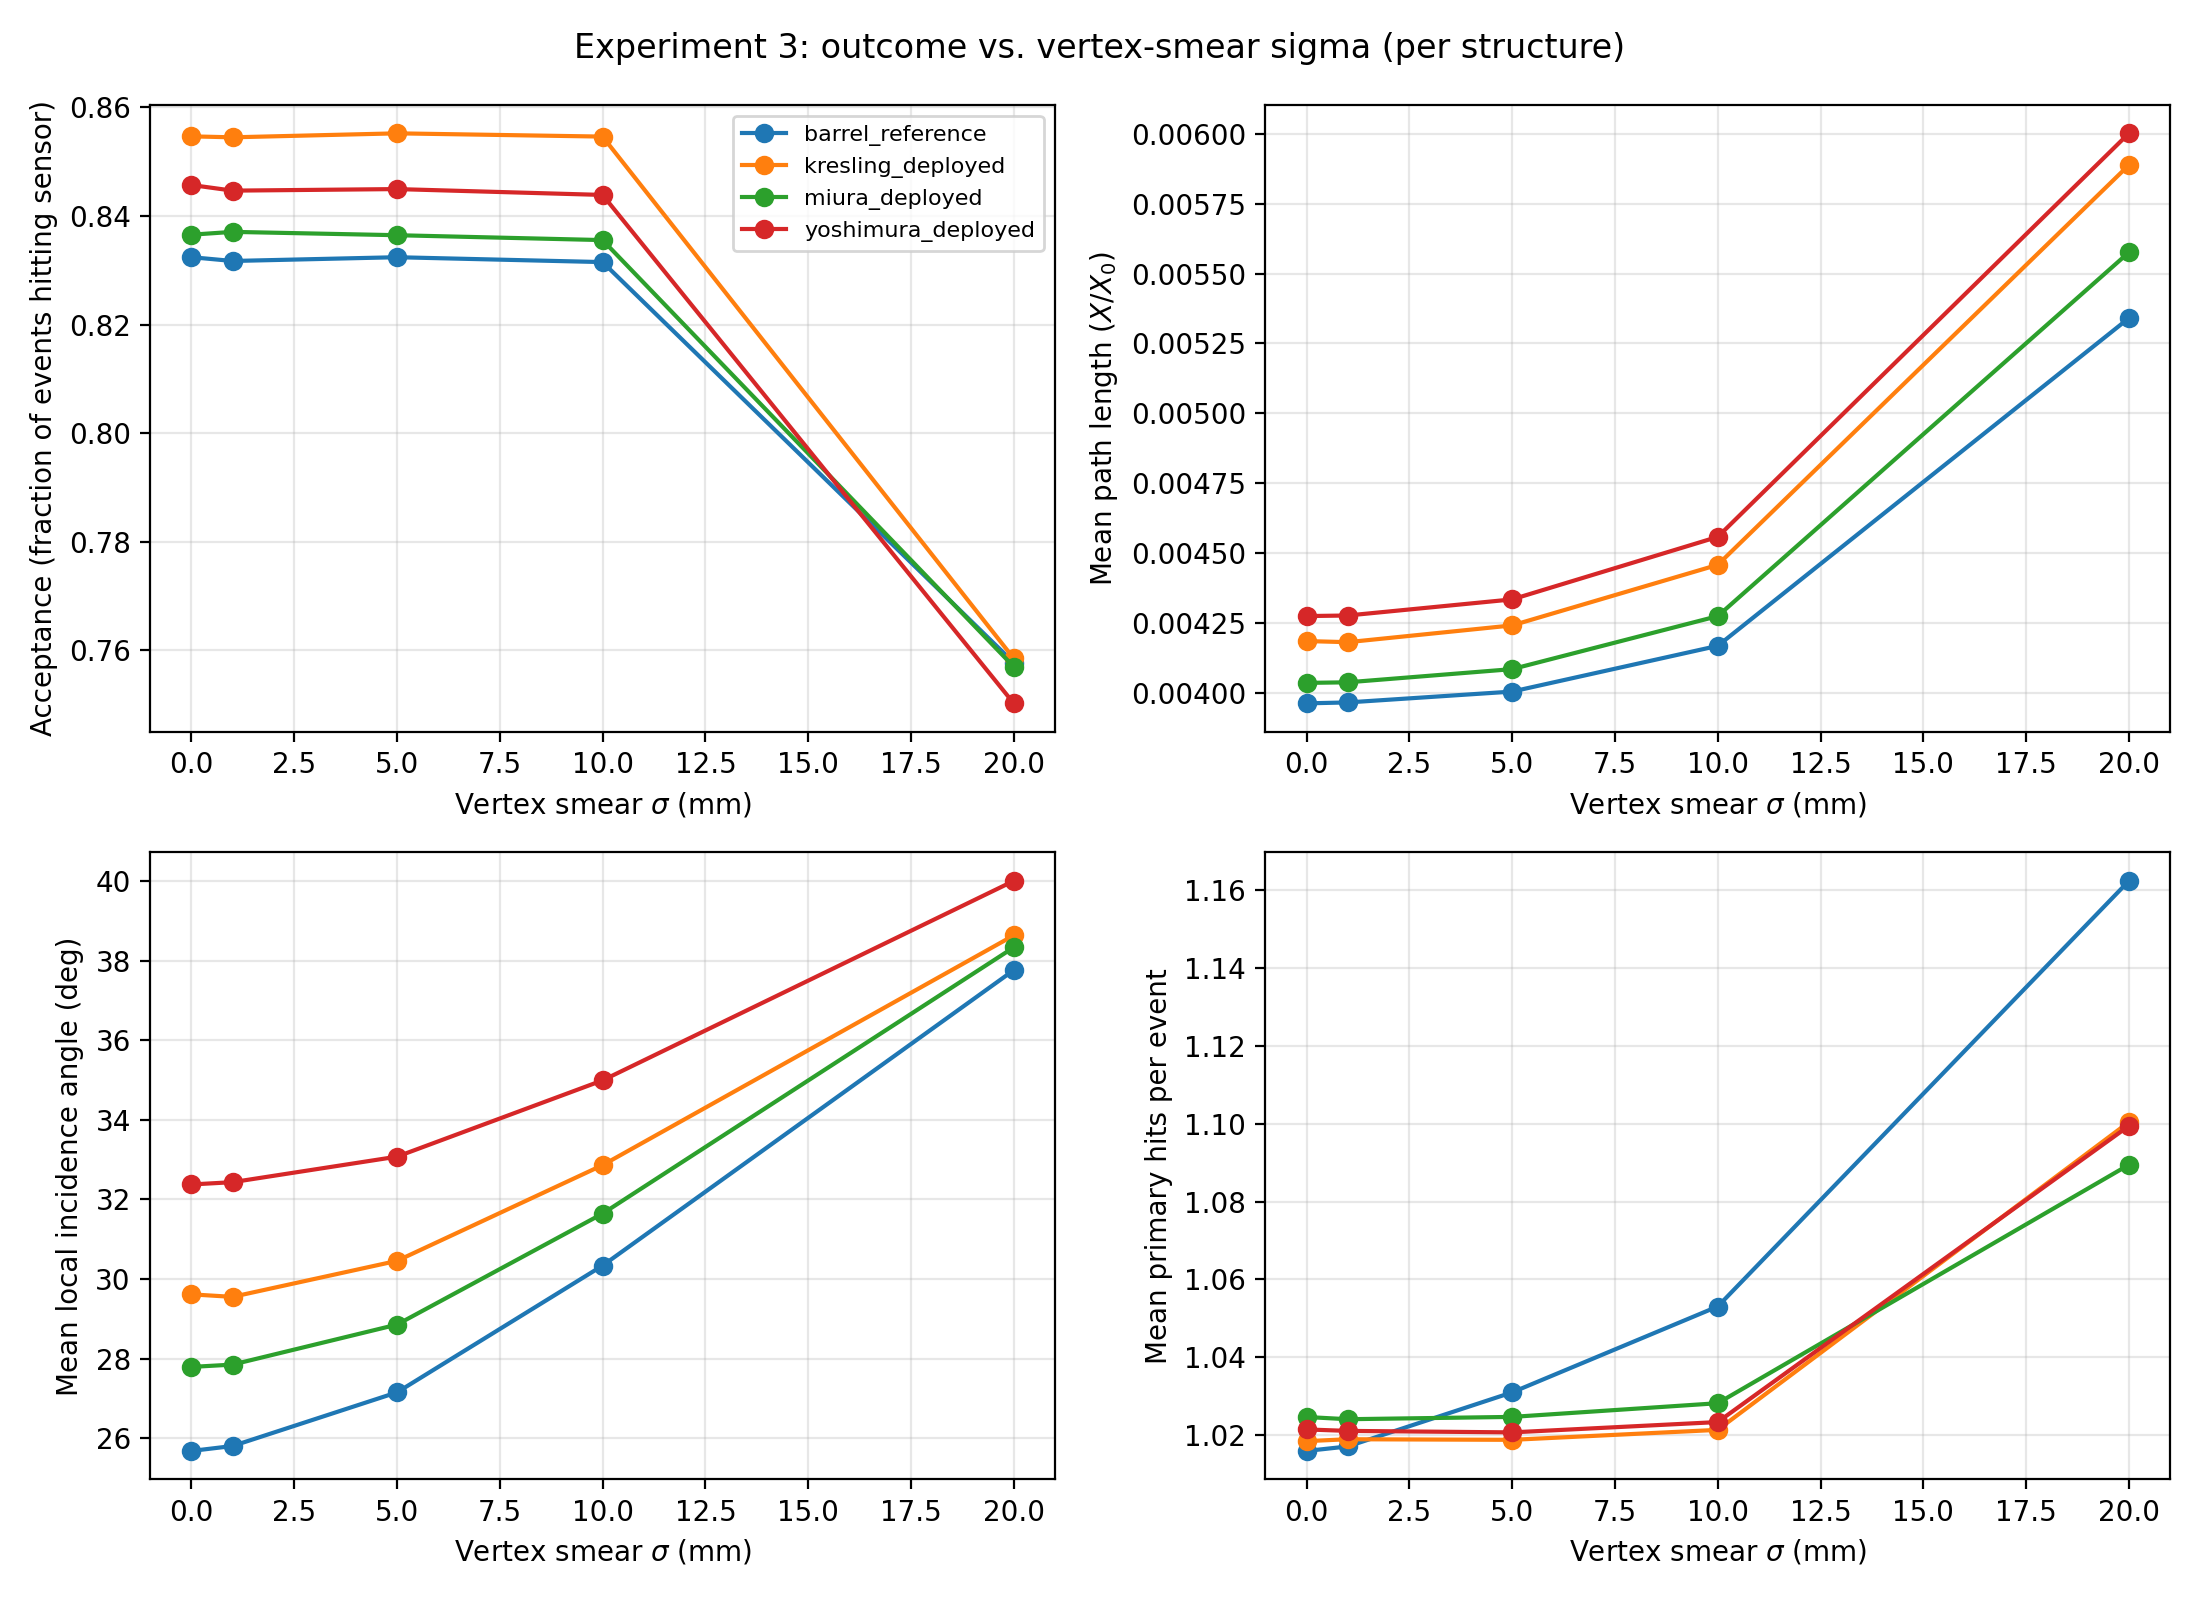
\includegraphics[width=\textwidth]{figures/fig_vertex_smear_sigma.png}
    \caption{Acceptance and $X_0$ vs.\ 3D Gaussian vertex smear width $\sigma$}
    \label{fig:smear_sigma}
\end{subfigure}\\[0.2em]
\begin{subfigure}[b]{0.68\textwidth}
    \centering
    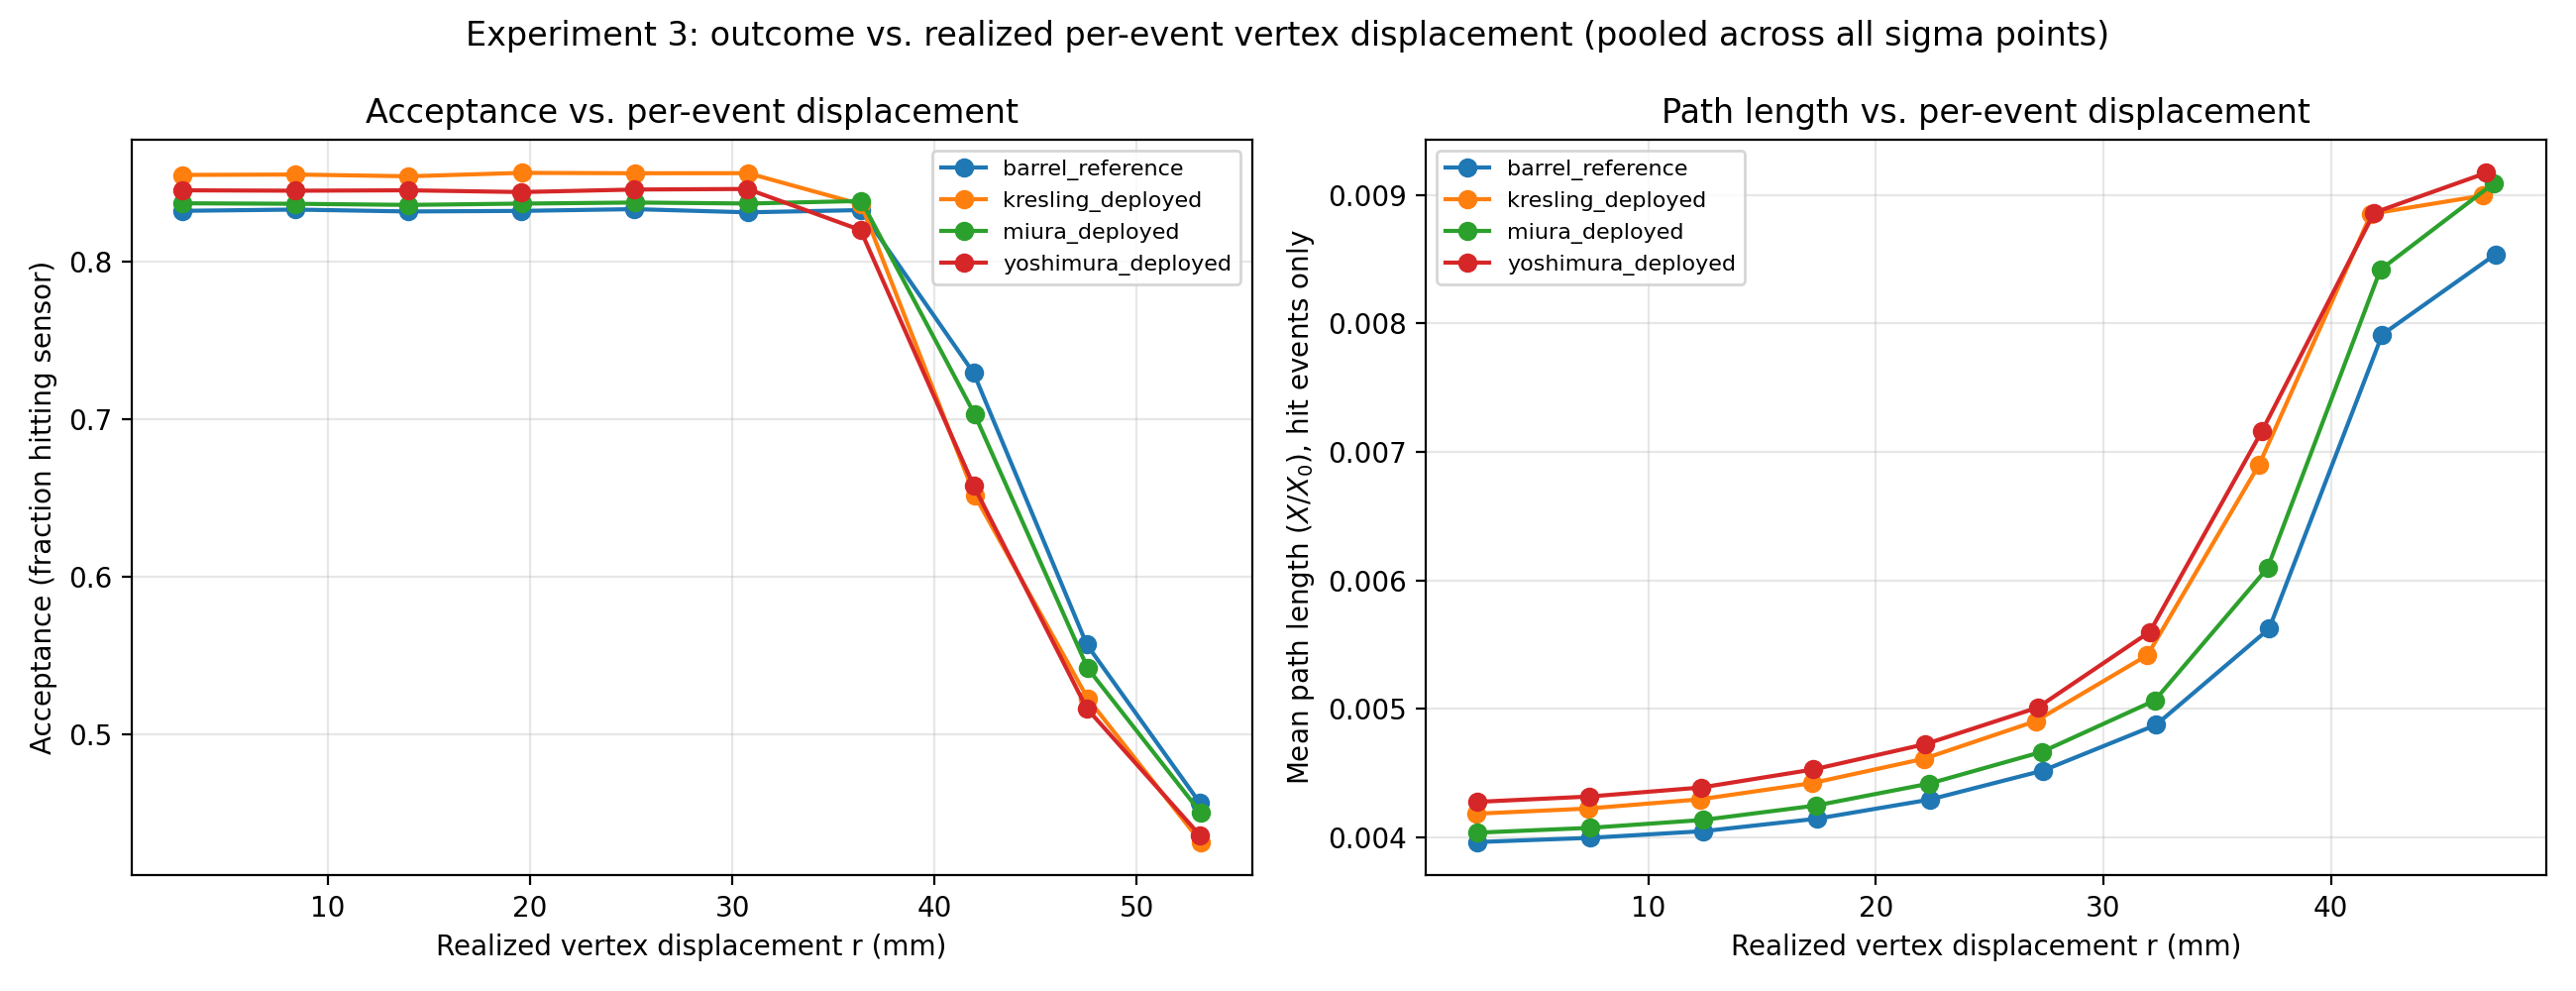
\includegraphics[width=\textwidth]{figures/fig_vertex_smear_displacement.png}
    \caption{Acceptance and $X_0$ vs.\ systematic radial vertex displacement}
    \label{fig:smear_disp}
\end{subfigure}
\caption{Vertex-position robustness evaluations: (a) Gaussian smear width $\sigma \in [0, 20]\text{ mm}$, and (b) systematic static radial displacement across geometries.}
\label{fig:vertex_smear}
\end{figure}

\FloatBarrier
\subsection{Relative Under-Coverage Fractions and Multi-Objective Pareto Frontier}
\label{sec:deadzone_pareto}

Table~\ref{tab:deadzone_multirun} reports the relative under-coverage fraction ($f_{\text{under}}$, $R < 0.5$) across five independent runs. The under-coverage ranking is inversely correlated with acceptance: Miura-ori exhibits negligible under-coverage ($0.041\%$), whereas Kresling ($1.451\%$) and Yoshimura ($1.861\%$) retain localized under-dense areas near fold seams. Figure~\ref{fig:deadzone_threshold} illustrates the under-coverage fraction across detection threshold sweeps from $0$ to $1$, confirming that at near-zero thresholds (absolute voids, $f_{\text{zero}}$), all geometries approach zero.

A key result from this sweep is that \textbf{no origami geometry contains any truly blind detection region} ($f_{\text{zero}} = 0.000\%$ for all three folds). True dead zones are defined as $({\theta}, z)$ bins with zero recorded hits across the full $500{,}000$-primary run, equivalent to threshold $R \to 0$. The threshold sweep confirms: non-zero fractions first emerge only at $R \approx 0.43$ (Miura-ori), $R \approx 0.31$ (Kresling), and $R \approx 0.26$ (Yoshimura) --- all well above zero. Regions counted by $f_{\text{under}}$ are suppressed-efficiency areas near fold seams where hit density falls below half the barrel reference, not geometrically blind voids. Reconstruction algorithms can compensate for relative efficiency dips through local hit weighting; they cannot recover truly uninstrumented regions. In this respect origami folding has a structural advantage over conventional tiled barrels, where physical inter-tile gaps create true blind zones ($f_{\text{zero}} > 0$) by design.

\begin{table}[!htbp]
\centering
\caption{Relative under-coverage fraction ($f_{\text{under}}$, $R < 0.5$) across five replication runs per fold geometry.}
\label{tab:deadzone_multirun}
\smallskip
\resizebox{\textwidth}{!}{
\begin{tabular}{lcccccccc}
\toprule
Structure & Run A & Run B & Run C & Run D & Run E & Mean & SD & SEM \\
\midrule
Miura-ori & 0.069\% & 0.069\% & 0.000\% & 0.069\% & 0.000\% & 0.041\% & 0.038\% & 0.017\% \\
Kresling  & 1.319\% & 1.597\% & 1.389\% & 1.667\% & 1.285\% & 1.451\% & 0.171\% & 0.076\% \\
Yoshimura & 1.771\% & 1.840\% & 1.632\% & 1.944\% & 2.118\% & 1.861\% & 0.183\% & 0.082\% \\
\bottomrule
\end{tabular}
}
\end{table}

Figure~\ref{fig:deadzone_threshold} displays the under-coverage fraction across a continuous sweep of the threshold ratio from $0$ to $1$. Across nearly the entire threshold range, the relative ordering of the geometries remains invariant, confirming that Miura-ori consistently provides the most spatially uniform coverage.

\begin{figure}[!htbp]
\centering
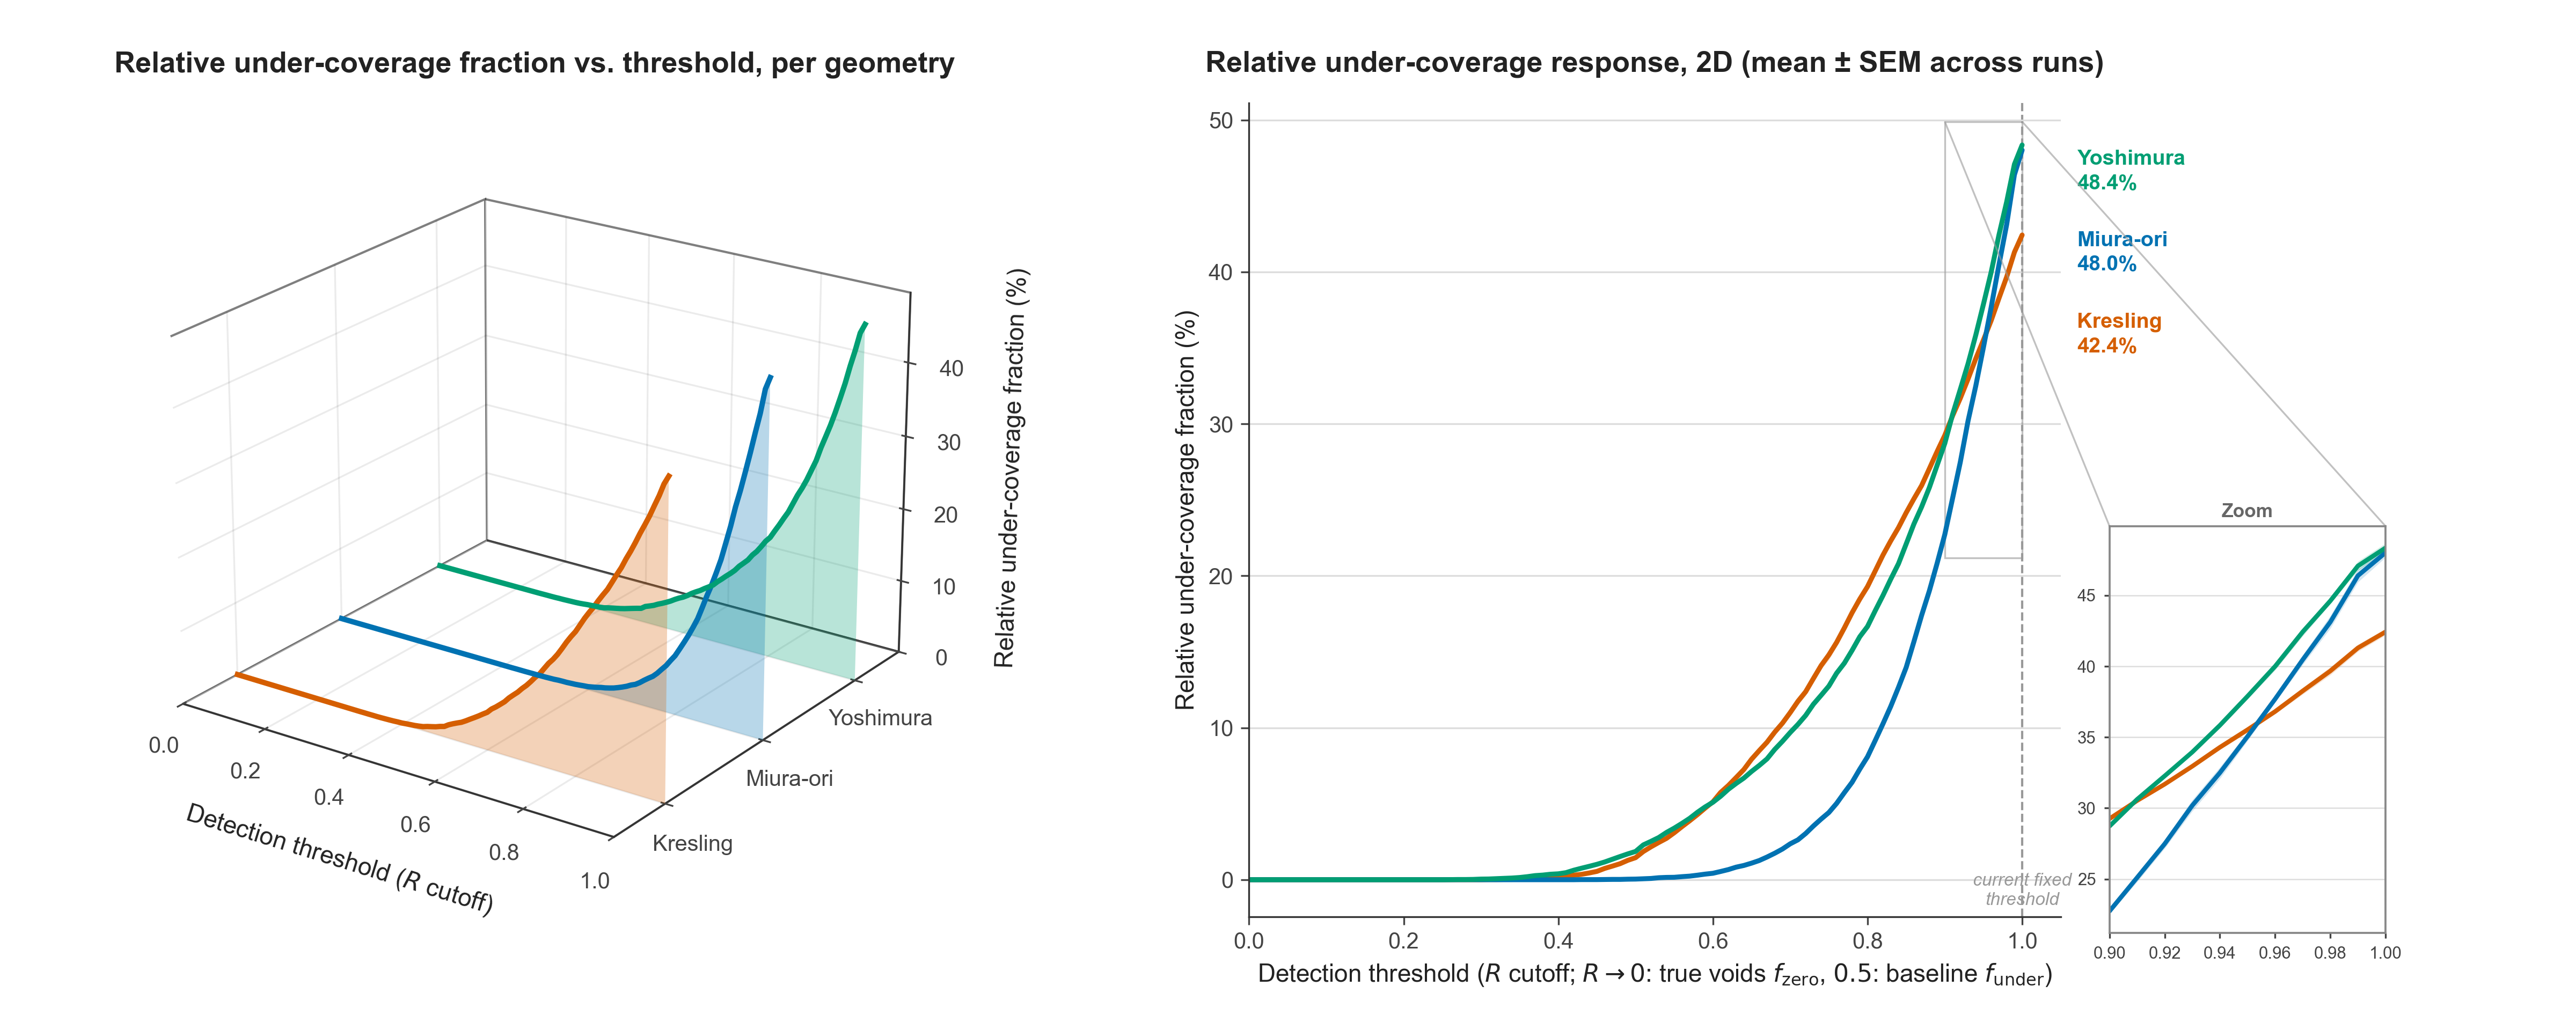
\includegraphics[width=0.88\textwidth]{figures/fig_deadzone_threshold_sweep.png}
\caption{Under-coverage fraction sensitivity across detection threshold parameters for candidate fold geometries, showing the 3D response surface (left) and 2D mean $\pm$ SEM comparison (right).}
\label{fig:deadzone_threshold}
\end{figure}

\begin{figure}[!htbp]
\centering
\begin{subfigure}[b]{0.48\textwidth}
    \centering
    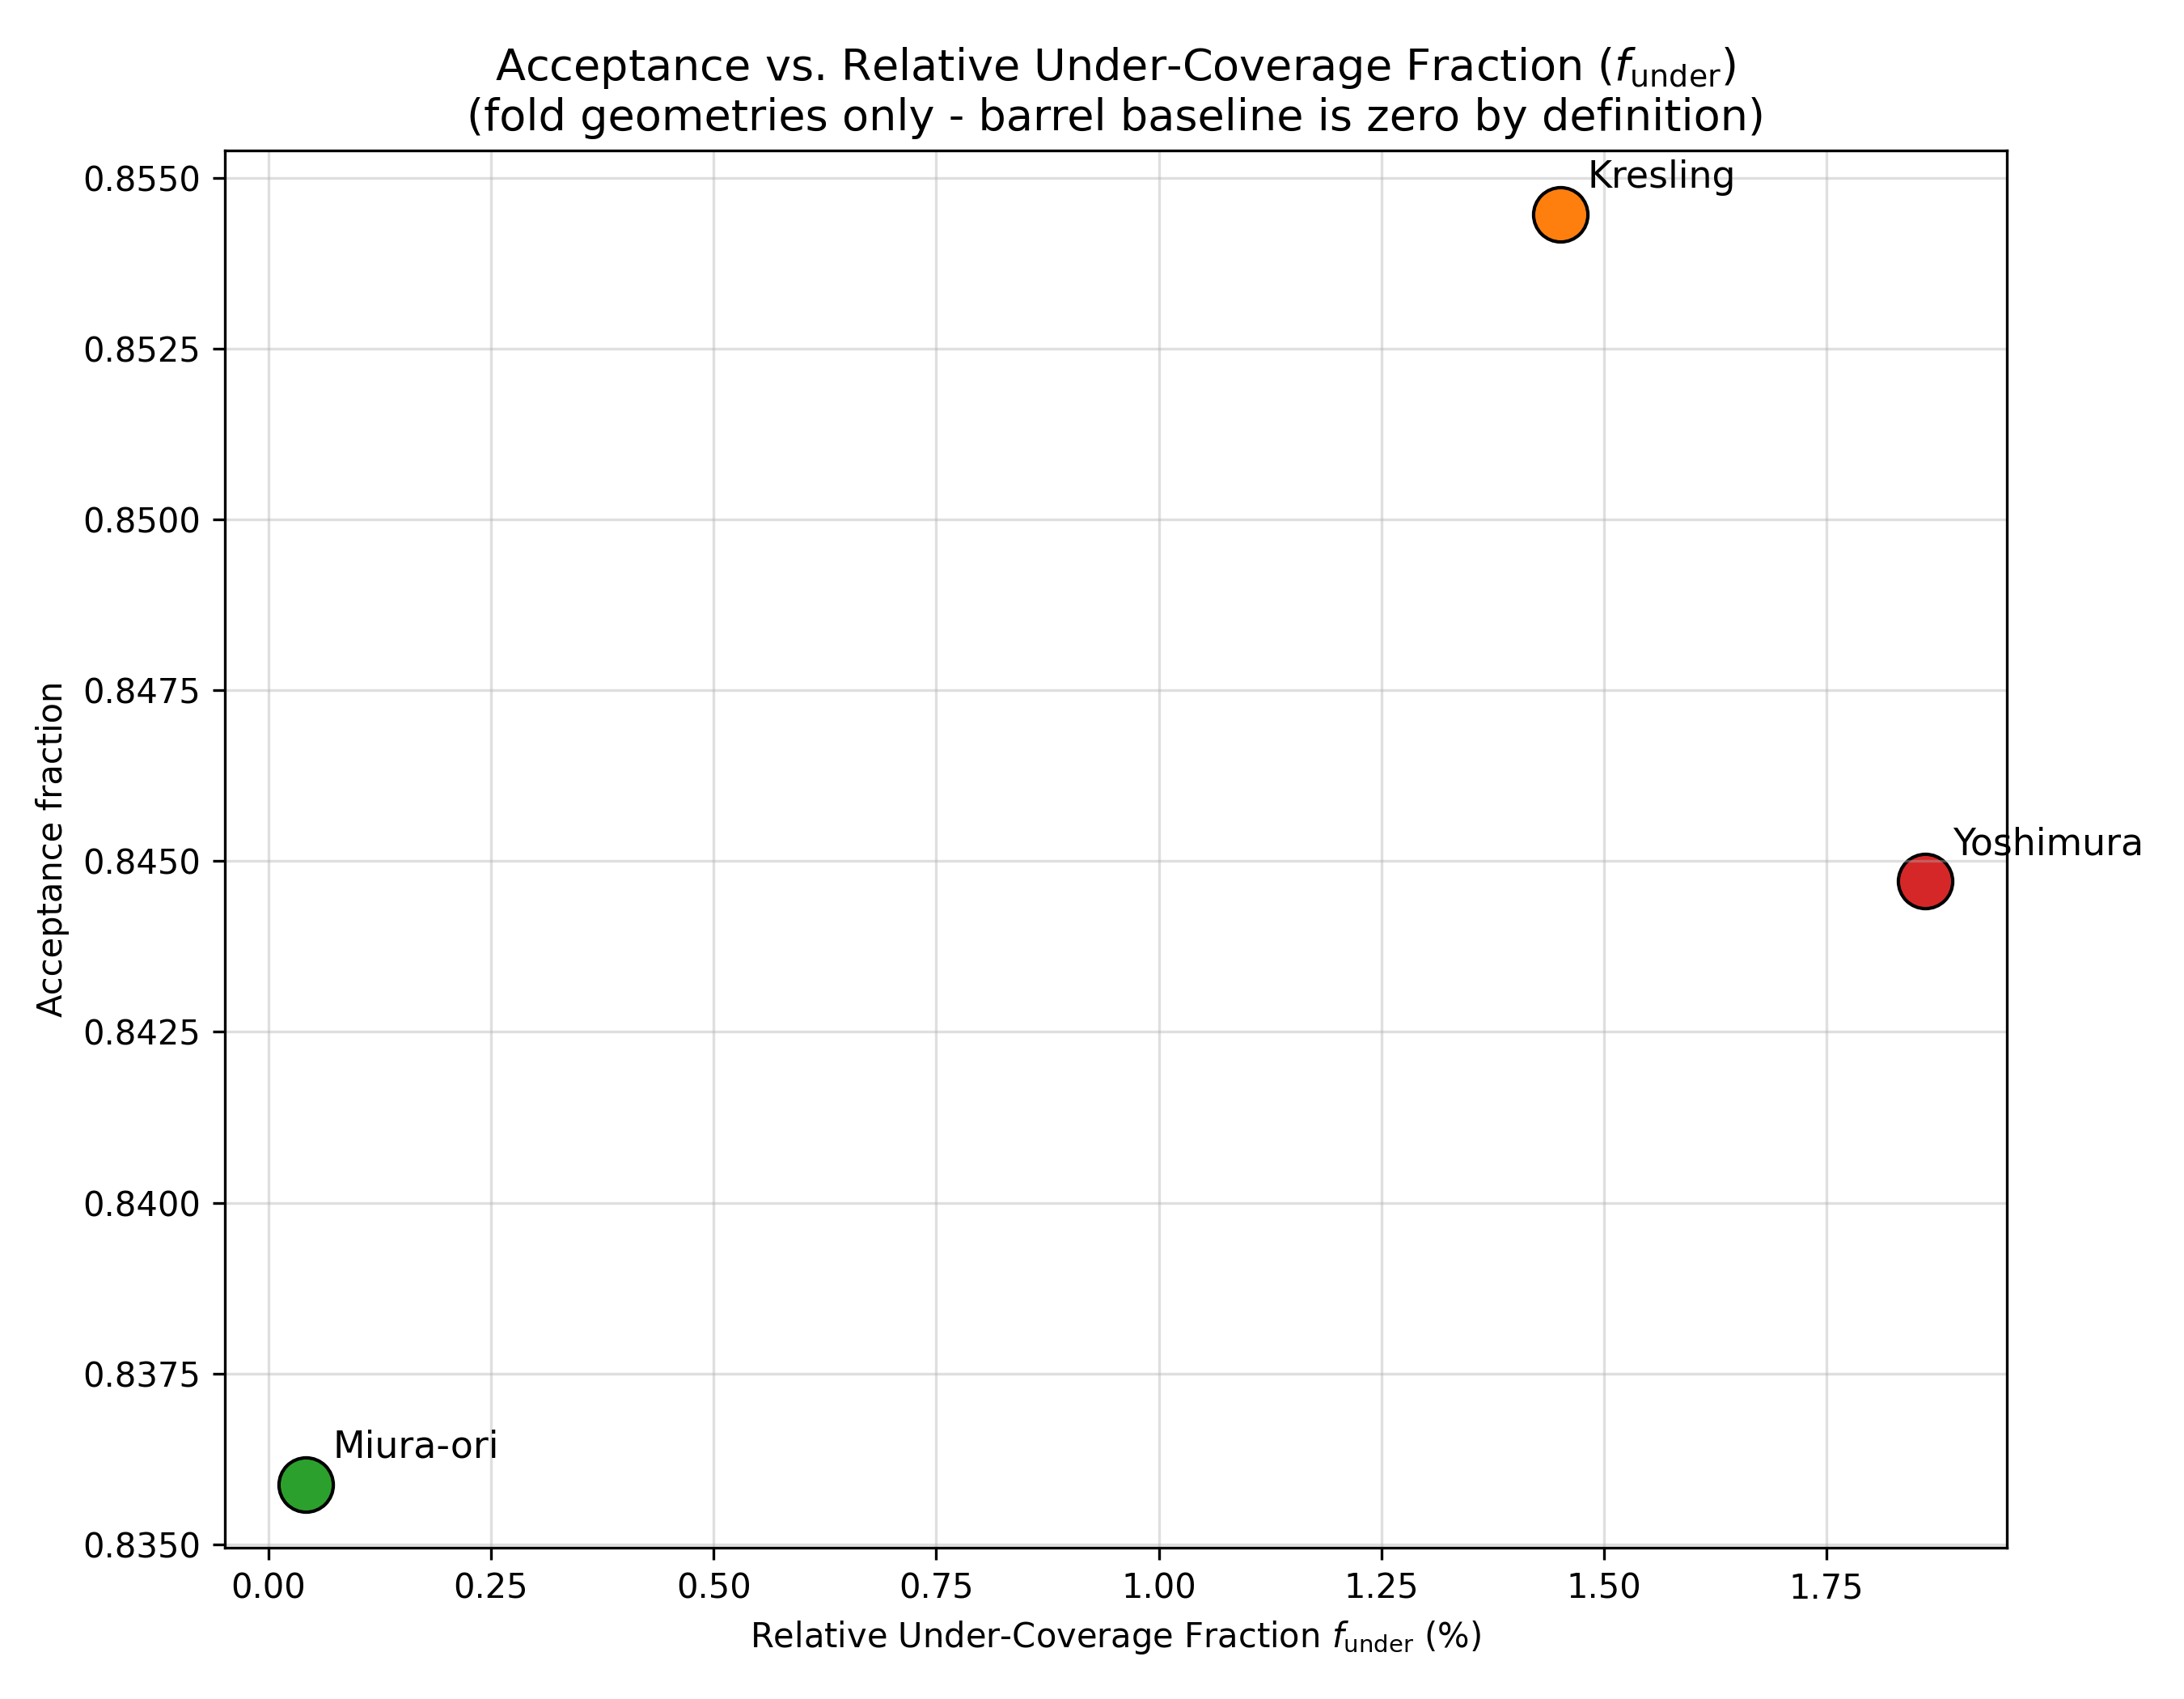
\includegraphics[width=\textwidth]{figures/fig6a_acceptance_vs_deadzone.png}
    \caption{Acceptance fraction vs.\ under-coverage fraction}
    \label{fig:pareto_a}
\end{subfigure}
\hfill
\begin{subfigure}[b]{0.48\textwidth}
    \centering
    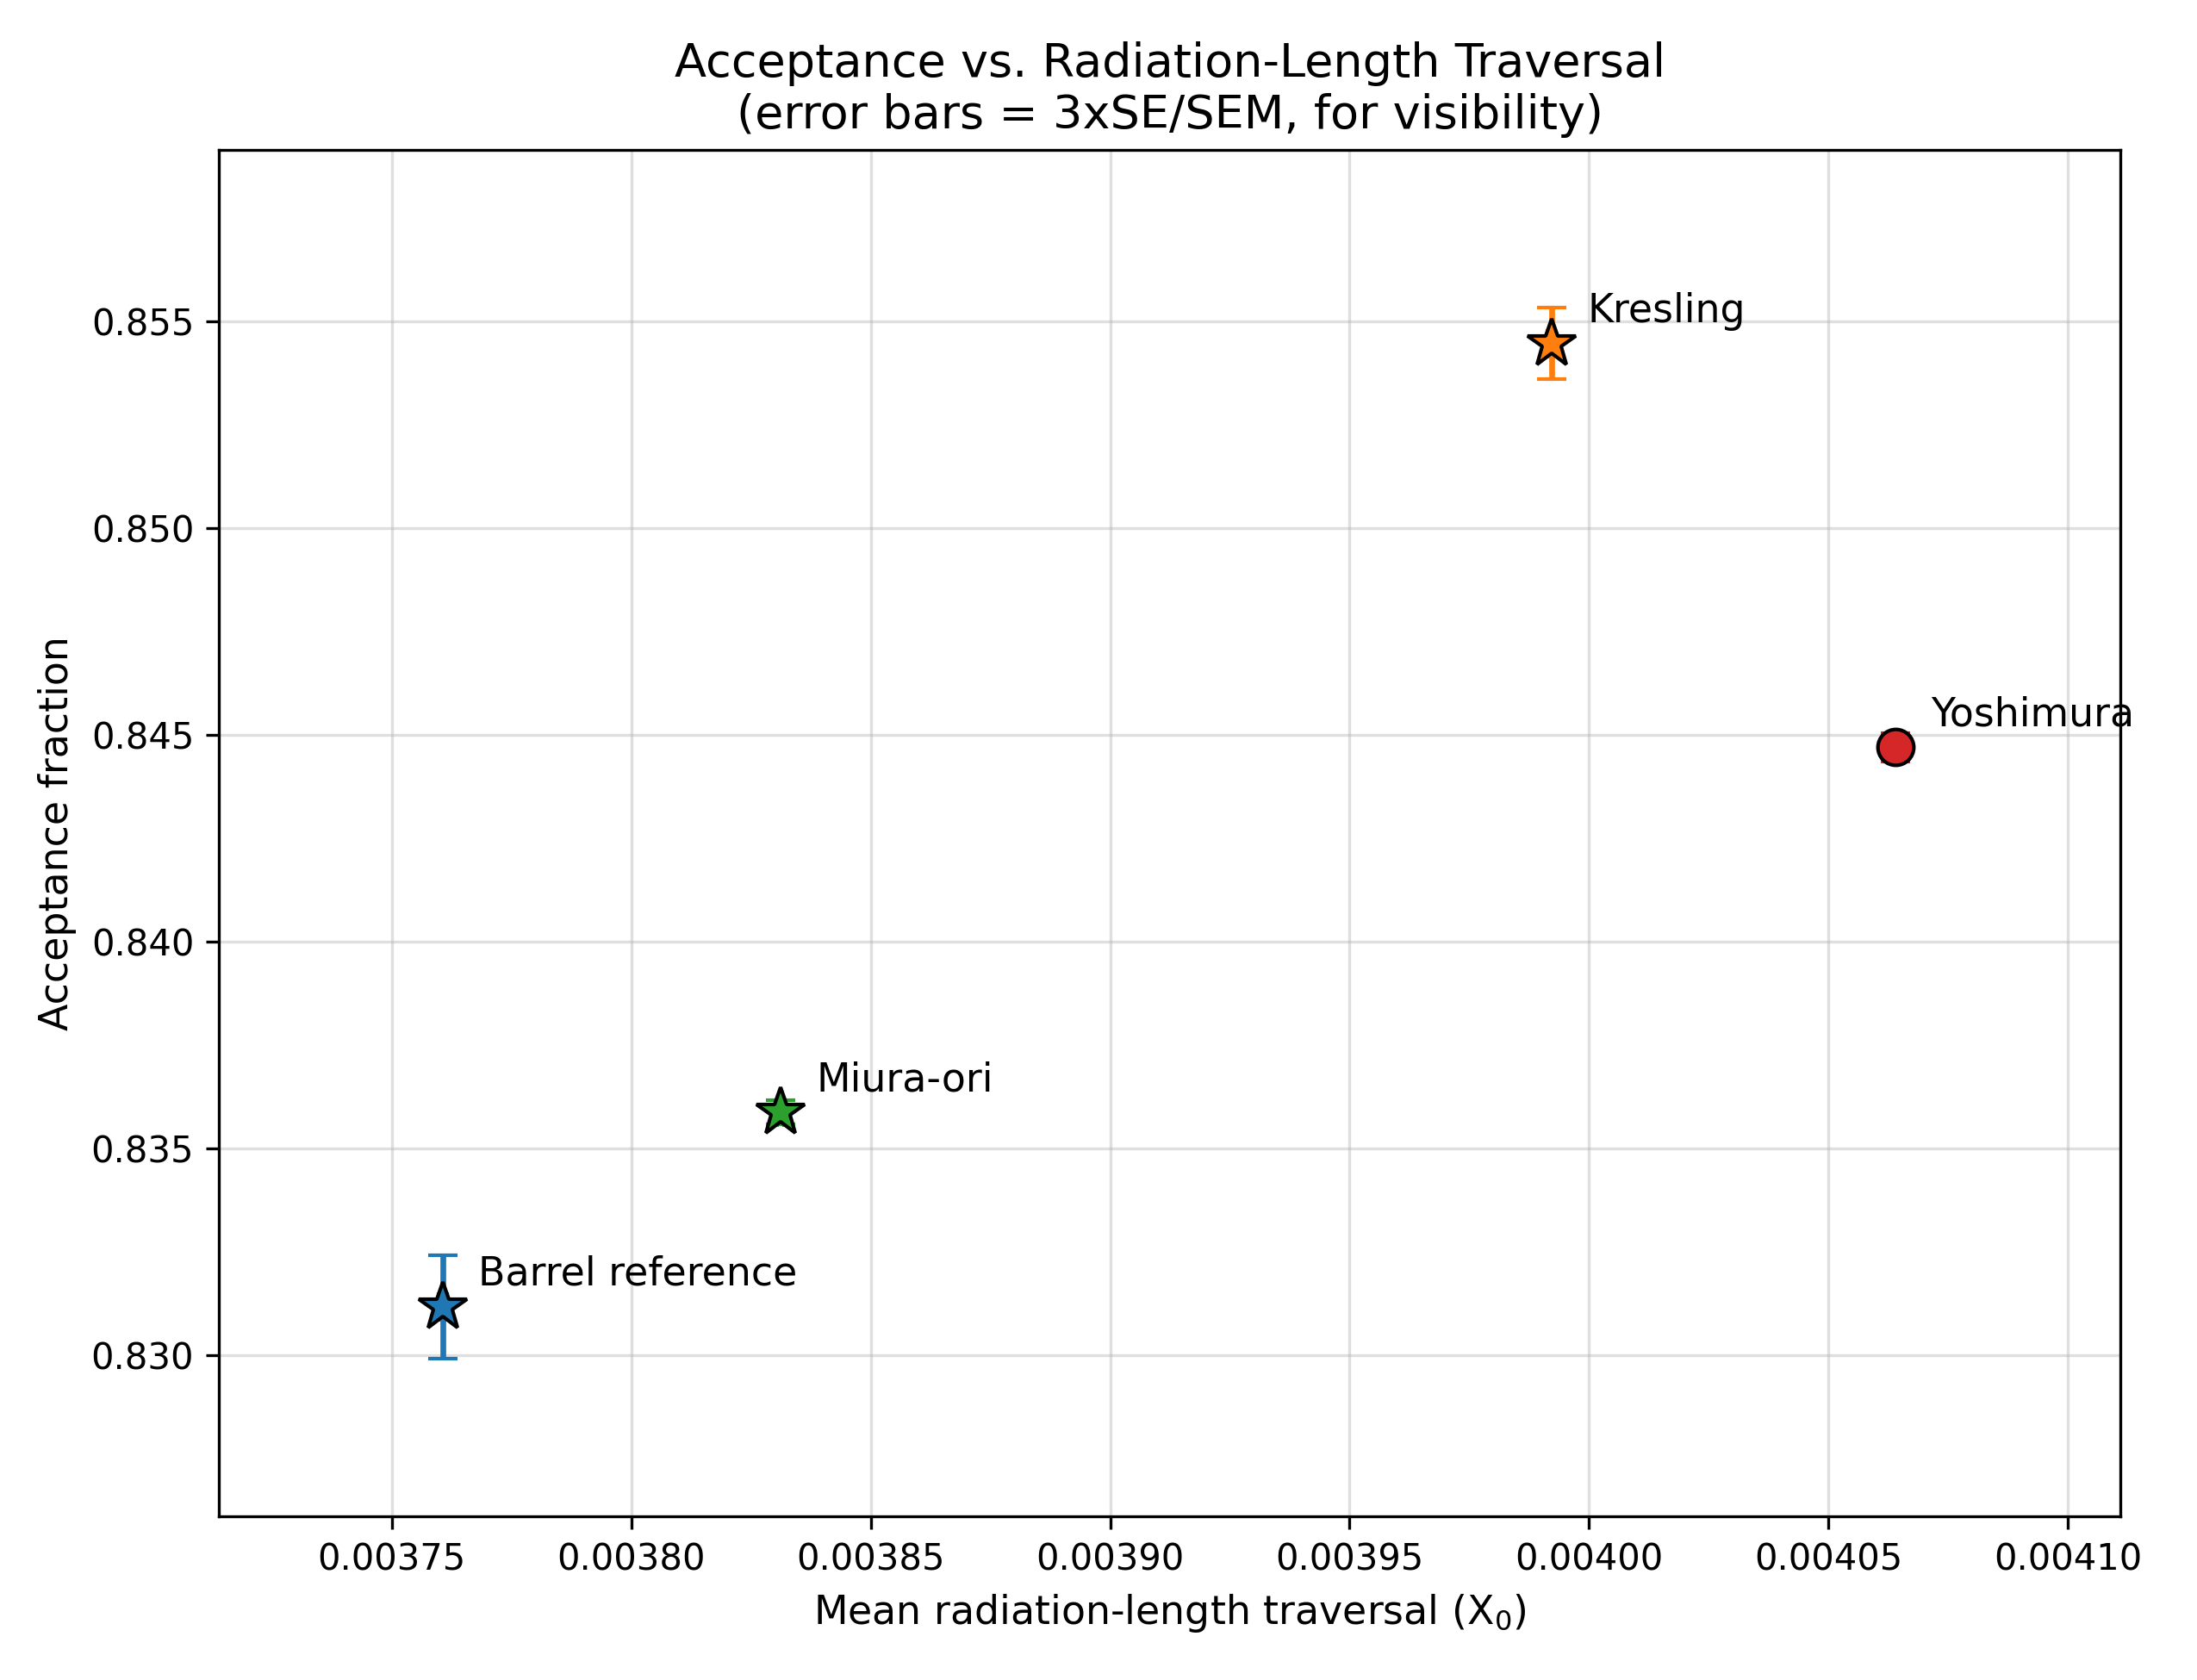
\includegraphics[width=\textwidth]{figures/fig6b_acceptance_vs_x0.png}
    \caption{Acceptance fraction vs.\ mean $X_0$}
    \label{fig:pareto_b}
\end{subfigure}
\caption{Pairwise 2D objective trade-off projections for acceptance: (a) acceptance fraction vs.\ under-coverage fraction, and (b) acceptance fraction vs.\ mean $X_0$.}
\label{fig:pareto_projections}
\end{figure}

\begin{figure}[!htbp]
\centering
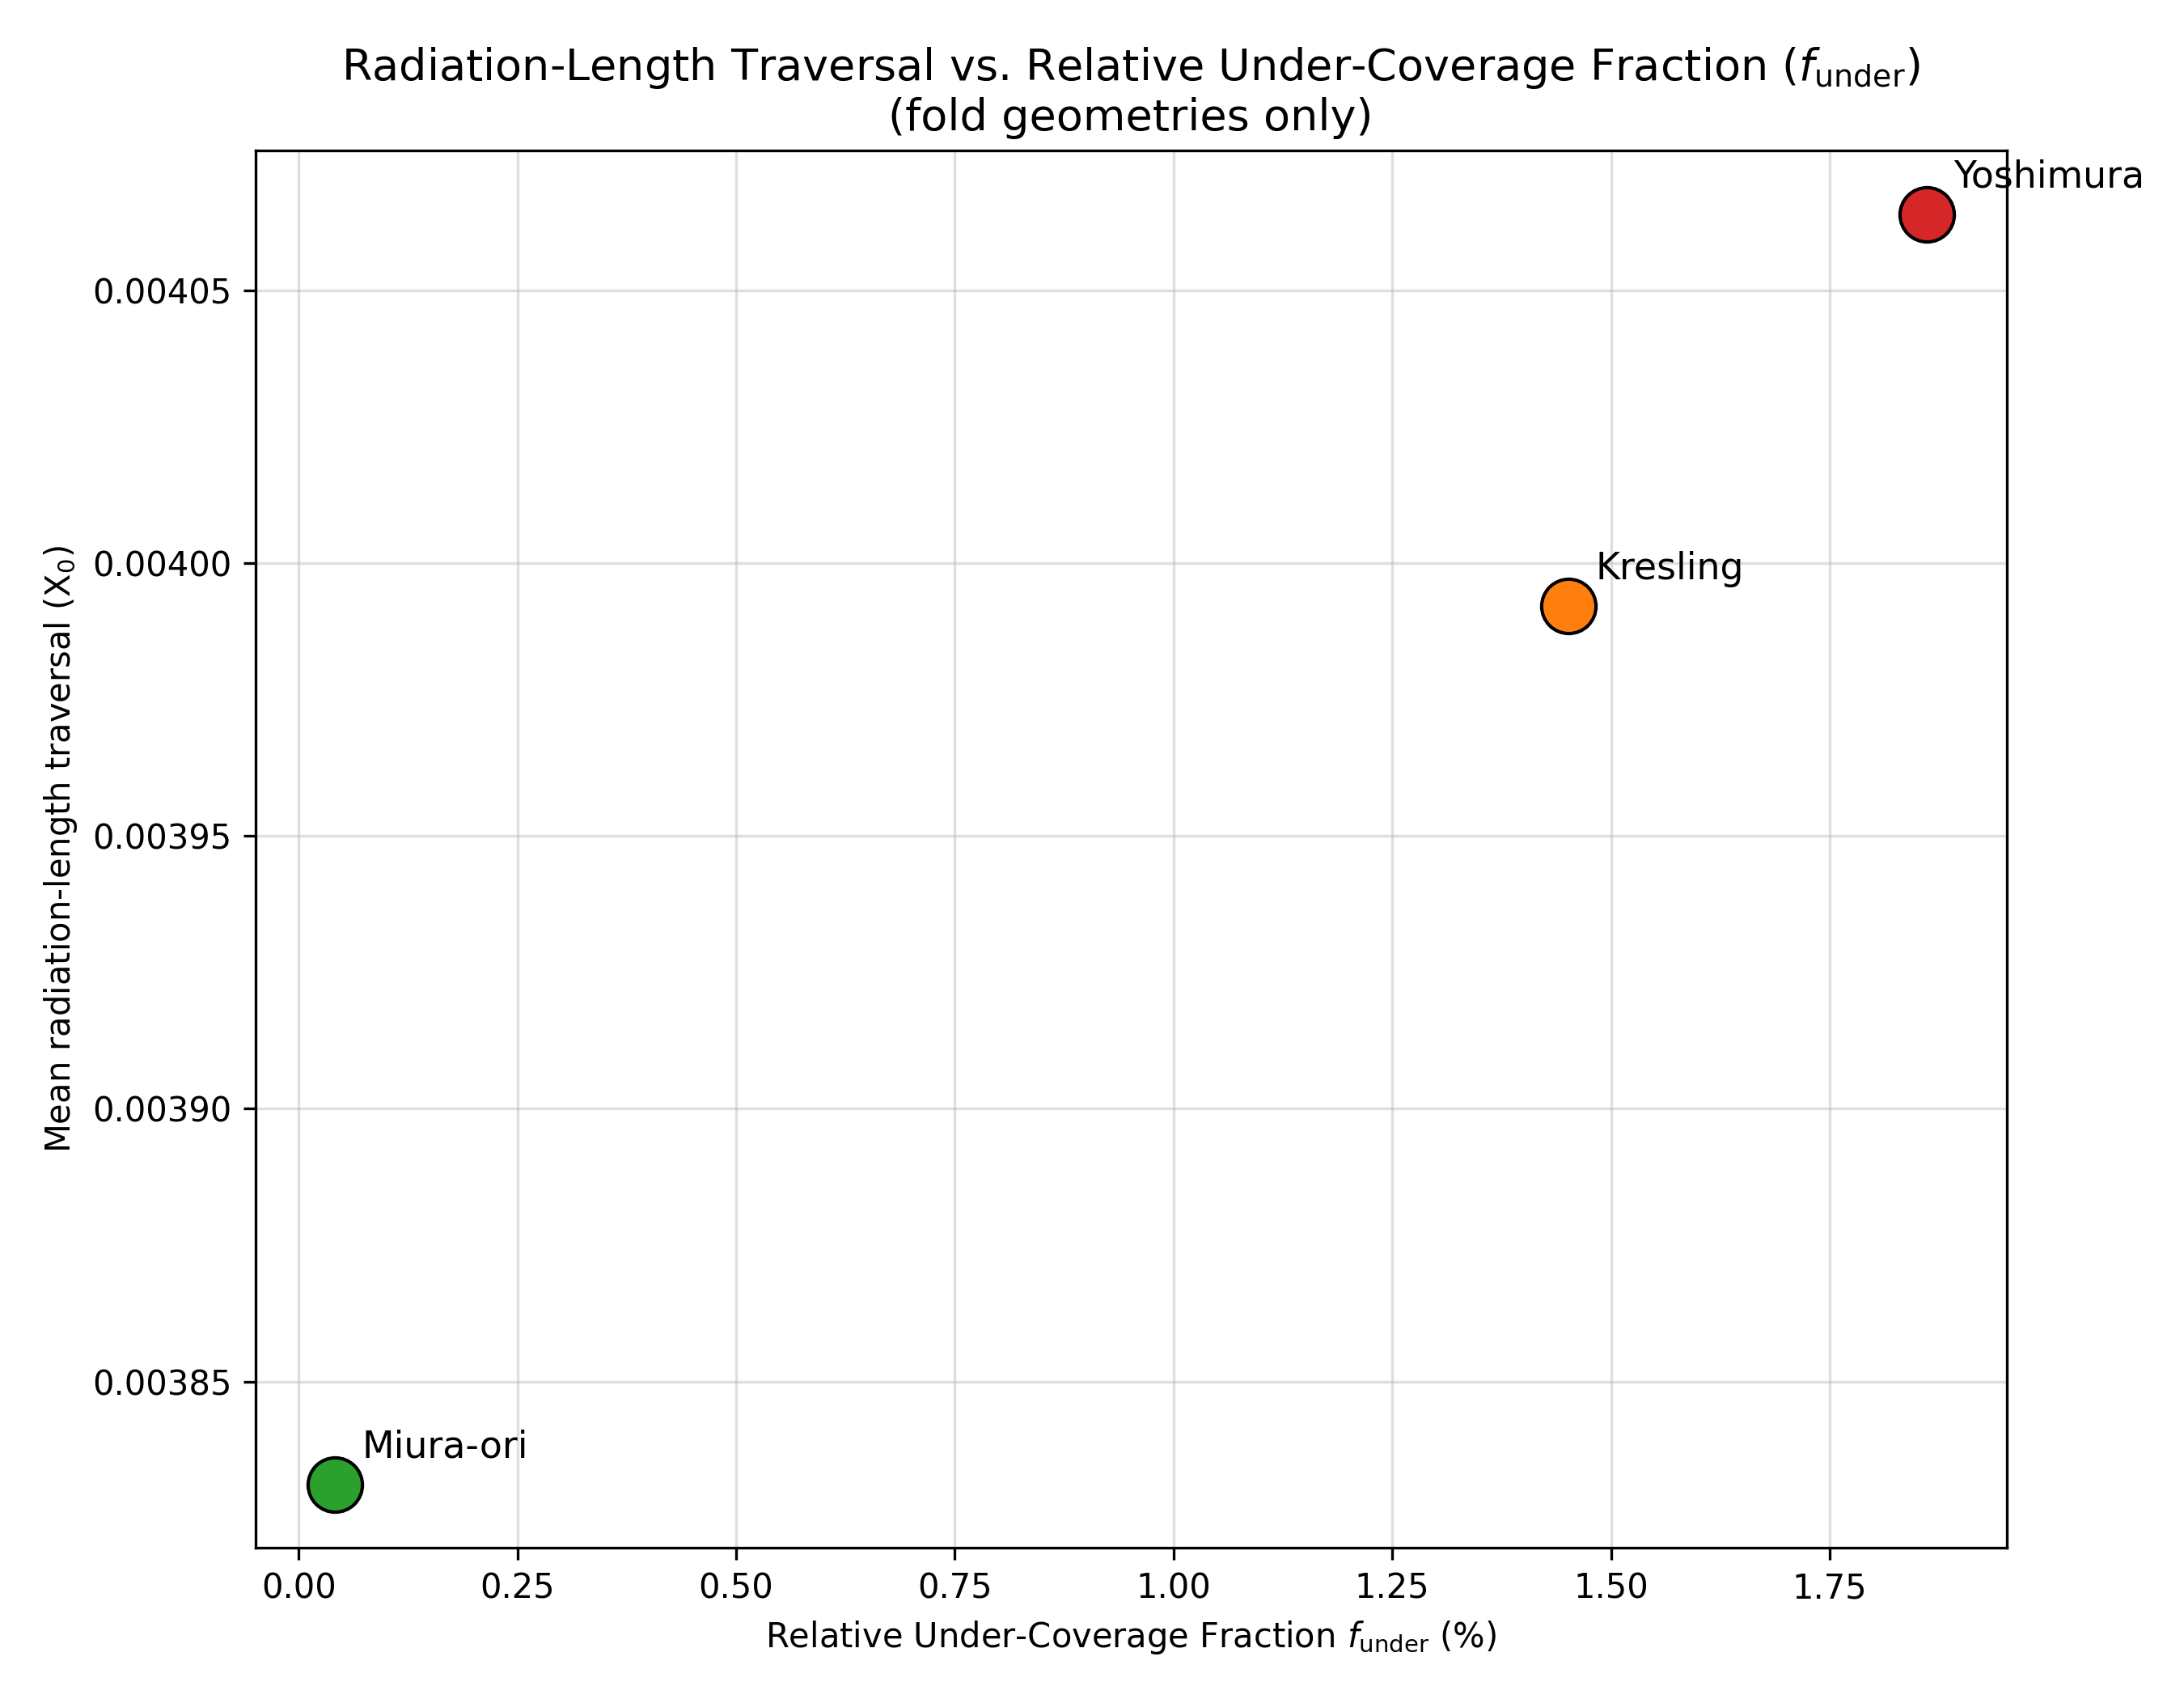
\includegraphics[width=0.52\textwidth]{figures/fig7_x0_vs_deadzone.png}
\caption{Mean radiation-length traversal $X_0$ versus under-coverage fraction across candidate fold geometries.}
\label{fig:pareto_c}
\end{figure}

\begin{figure}[!htbp]
\centering
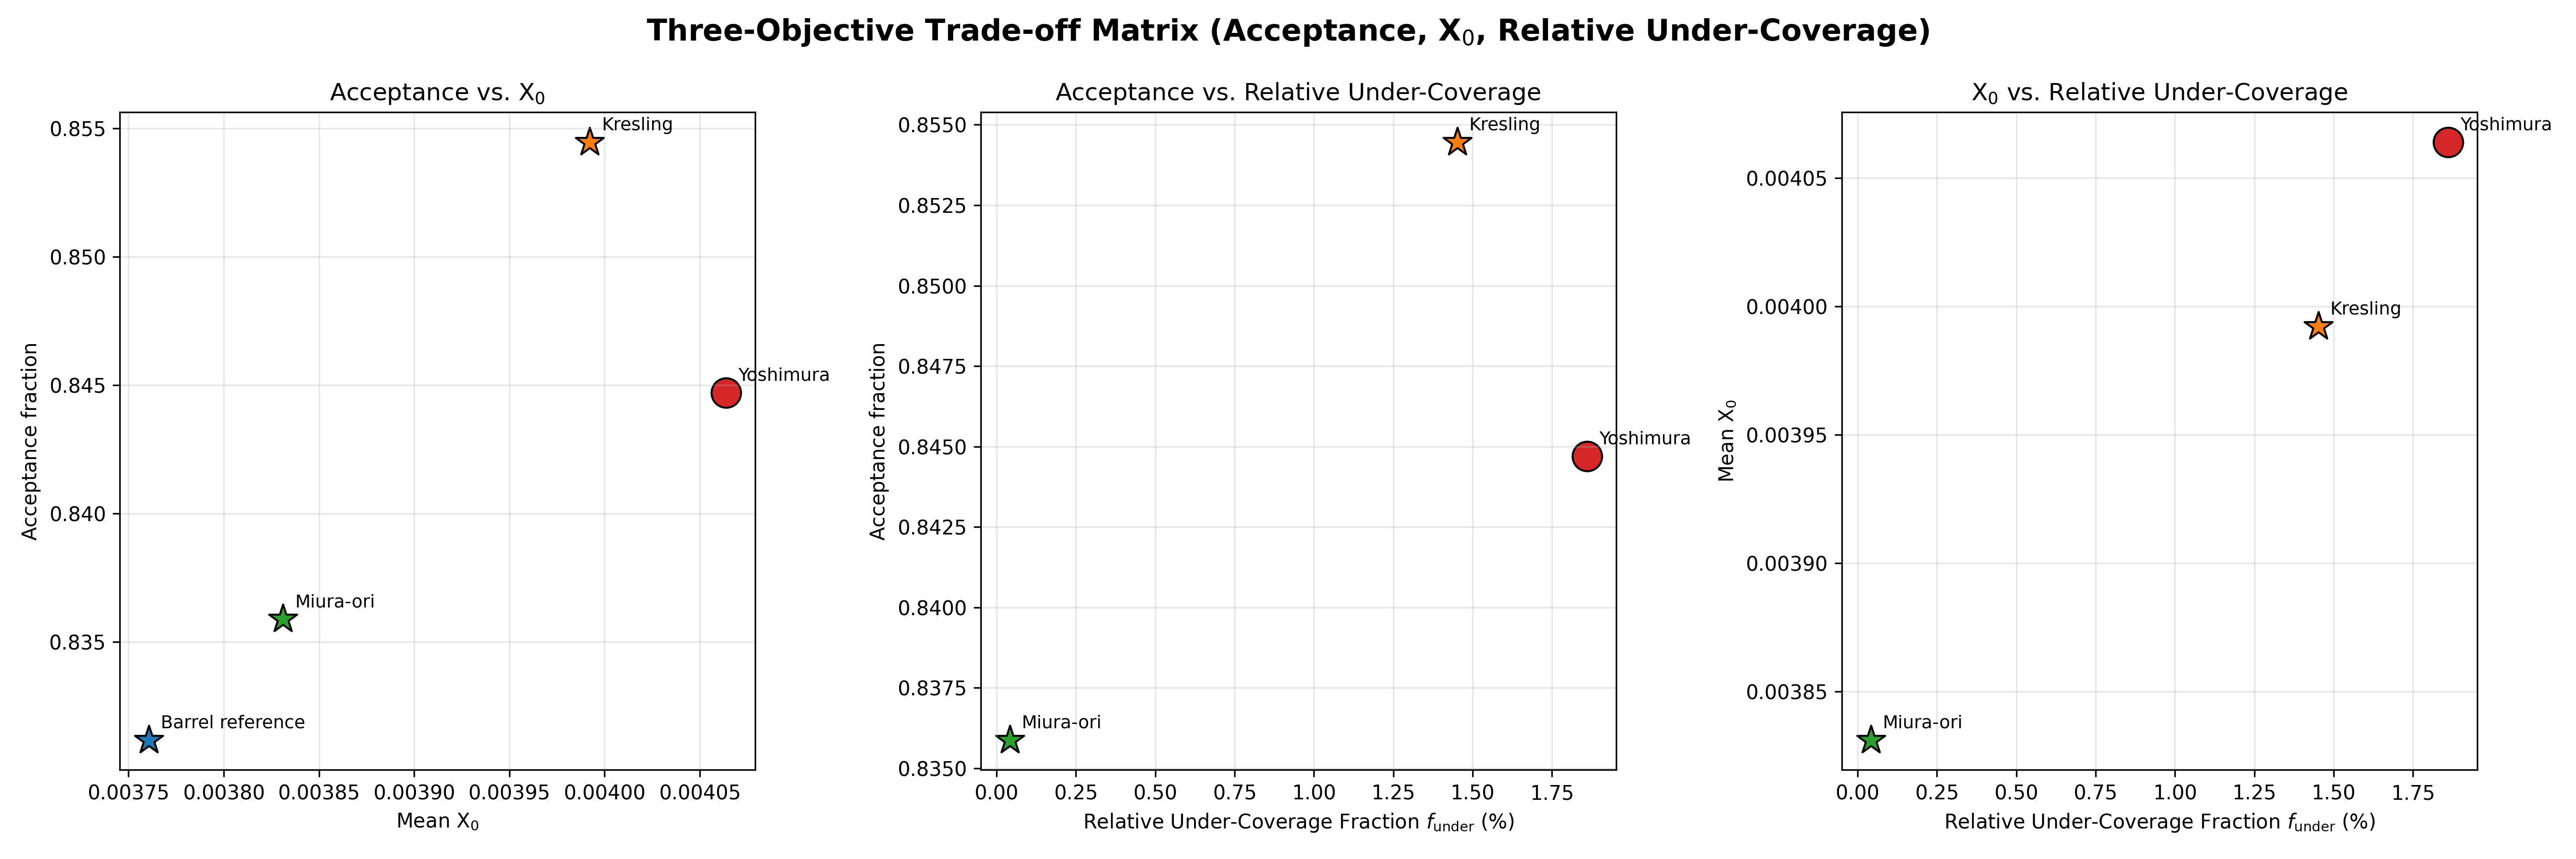
\includegraphics[width=0.88\textwidth]{figures/fig8_tradeoff_matrix.png}
\caption{Comprehensive three-panel trade-off matrix pairing acceptance fraction, mean $X_0$, and under-coverage fraction for all geometries.}
\label{fig:tradeoff_matrix}
\end{figure}

\begin{figure}[!htbp]
\centering
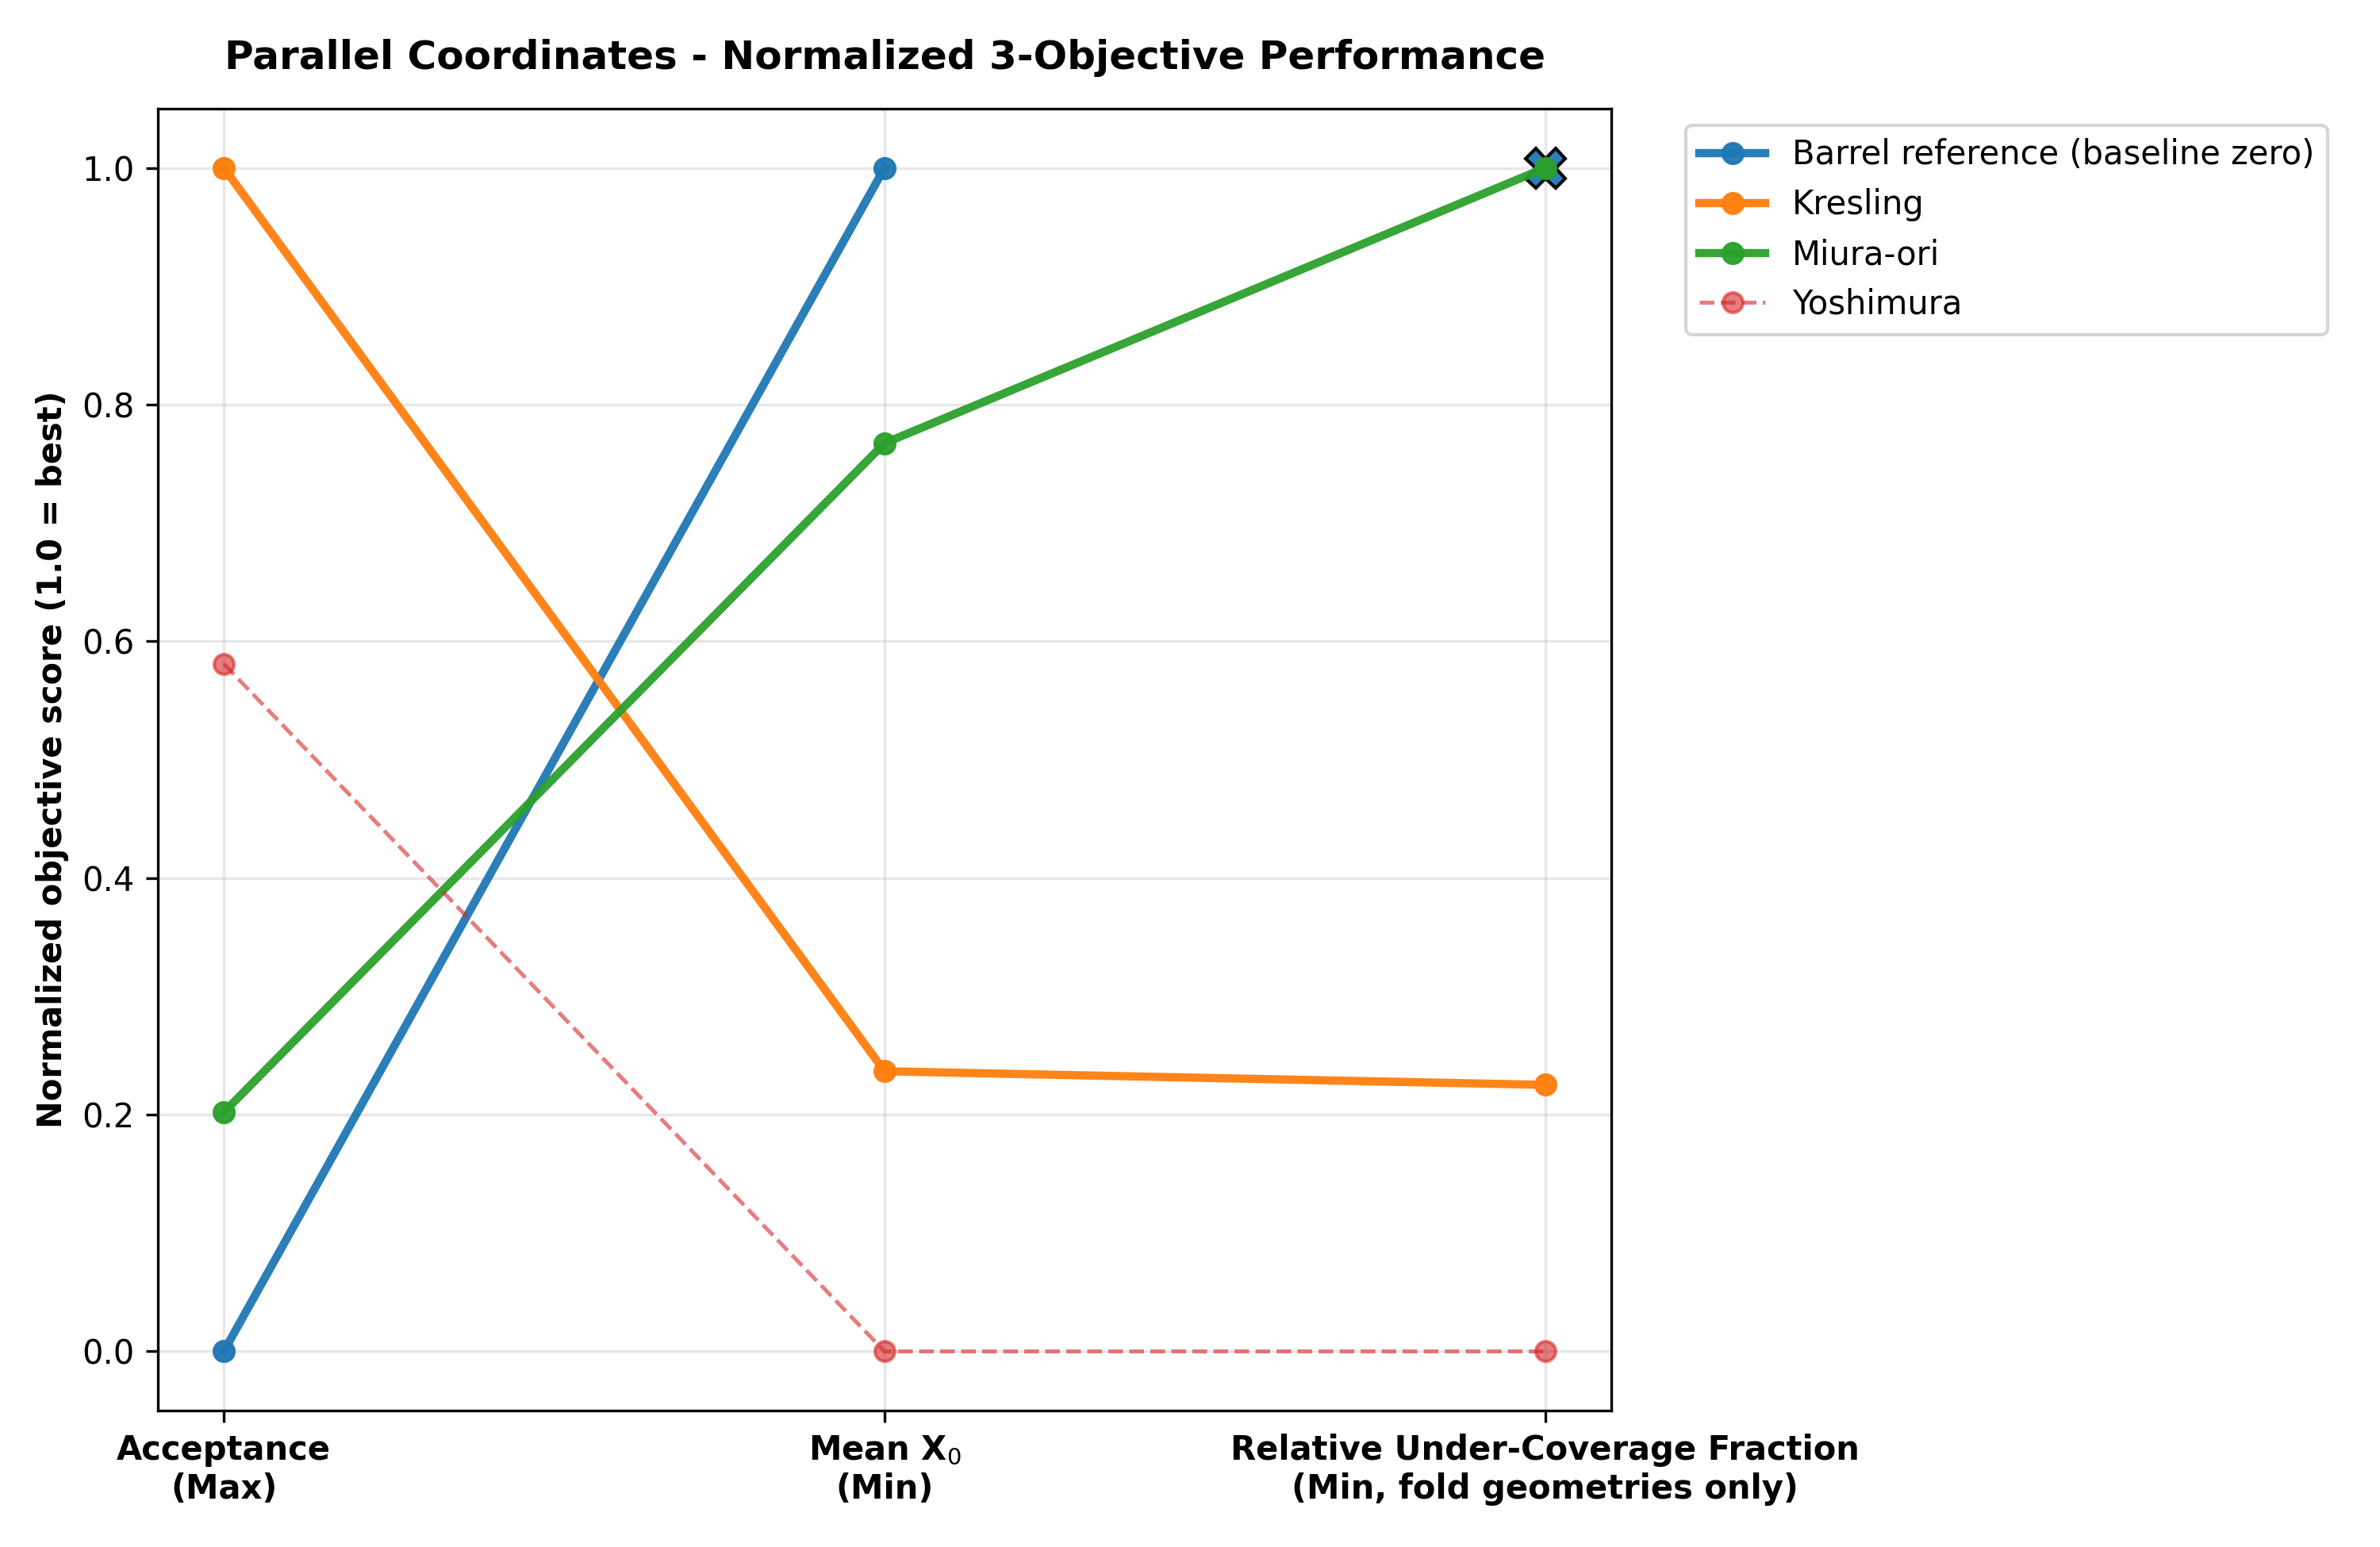
\includegraphics[width=0.56\textwidth]{figures/fig9_parallel_coords.png}
\caption{Parallel coordinate representation across normalized performance objectives (where upward orientation denotes superior performance).}
\label{fig:parallel_coords}
\end{figure}

Figures~\ref{fig:pareto_projections}--\ref{fig:parallel_coords} demonstrate that the four geometries constitute a classic Pareto set (quoted performance figures correspond to the 5-run replication means in Table~\ref{tab:multirun_results}):
\begin{itemize}
    \item \textbf{Kresling} maximizes acceptance ($A = 85.54\%$) at intermediate material cost ($X/X_0 = 4.20 \times 10^{-3}$).
    \item \textbf{Miura-ori} minimizes material penalty ($X/X_0 = 4.05 \times 10^{-3}$) and nearly eliminates under-coverage ($f_{\text{under}} = 0.04\%$) with modest acceptance gain ($A = 83.67\%$).
    \item \textbf{Yoshimura} is Pareto-dominated, incurring both the highest material cost ($X/X_0 = 4.30 \times 10^{-3}$) and highest under-coverage fraction ($f_{\text{under}} = 1.86\%$) for inferior acceptance ($84.48\%$).
\end{itemize}

\FloatBarrier
\subsection{Spatial Structure of Under-Coverage and Overlaps}
\label{sec:spatial_structure}

Two-dimensional $(\theta, z)$ hit-density and material maps (Figures~\ref{fig:map_miura}--\ref{fig:map_kresling}) elucidate the spatial mechanism:
\begin{itemize}
    \item \textbf{Miura-ori (Figure~\ref{fig:map_miura}):} Displays a smooth, quasi-uniform hit-density profile ($R \approx 1$) and continuous material gradient, matching its low under-coverage fraction.
    \item \textbf{Yoshimura (Figure~\ref{fig:map_yoshimura}):} Shows sharp periodic diamond bands where overlap seams ($R > 1.5$) alternate with localized under-dense valleys ($R < 1$).
    \item \textbf{Kresling (Figure~\ref{fig:map_kresling}):} Exhibits helical band structures with localized material peaks at fold vertices.
\end{itemize}

\begin{figure}[!htbp]
\centering
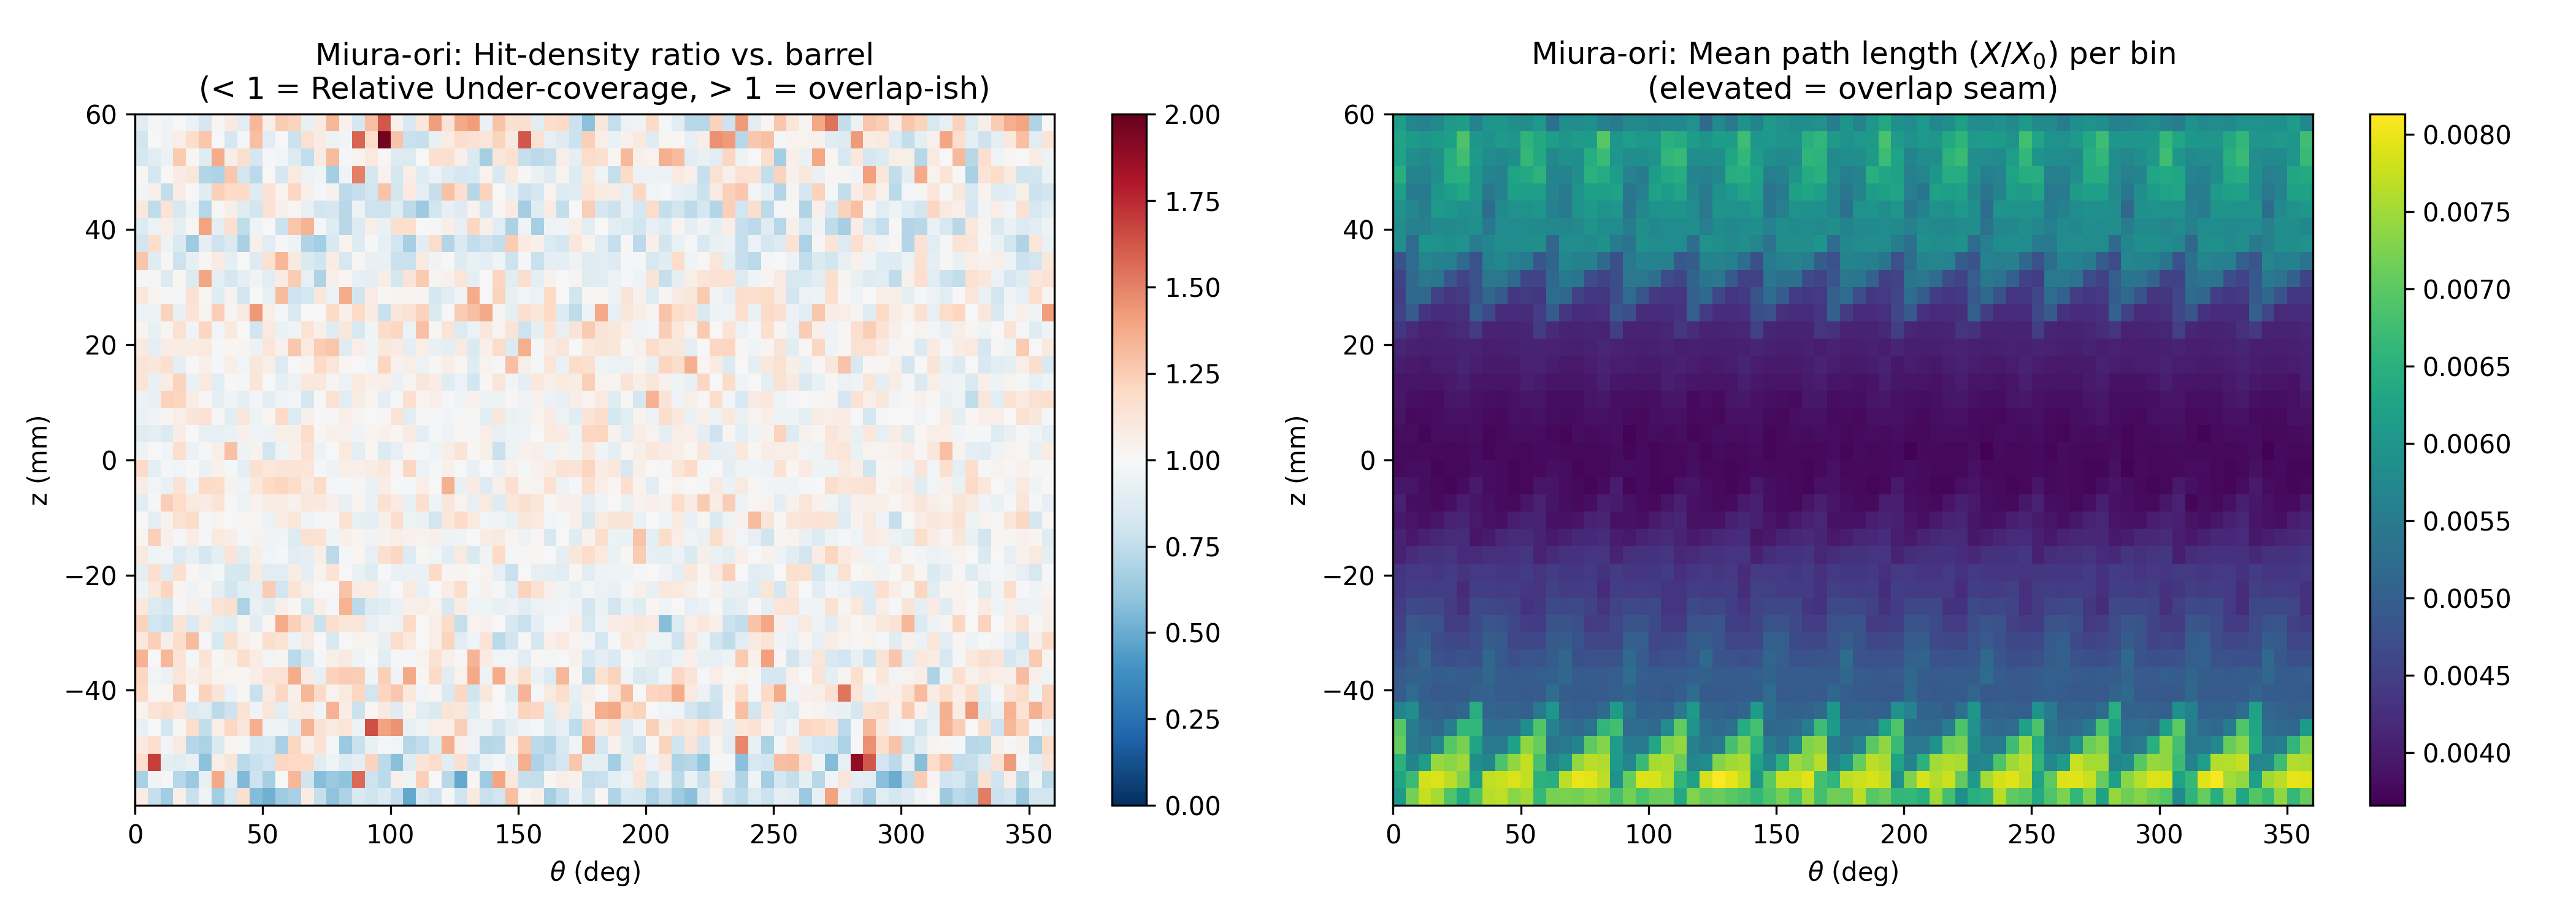
\includegraphics[width=0.86\textwidth]{figures/fig10_map_miura.png}
\caption{Spatial hit-density enhancement ratio $R(\theta, z)$ (left) and mean $X_0$ (right) for Cylindrical Miura-ori relative to the barrel control.}
\label{fig:map_miura}
\end{figure}

\begin{figure}[!htbp]
\centering
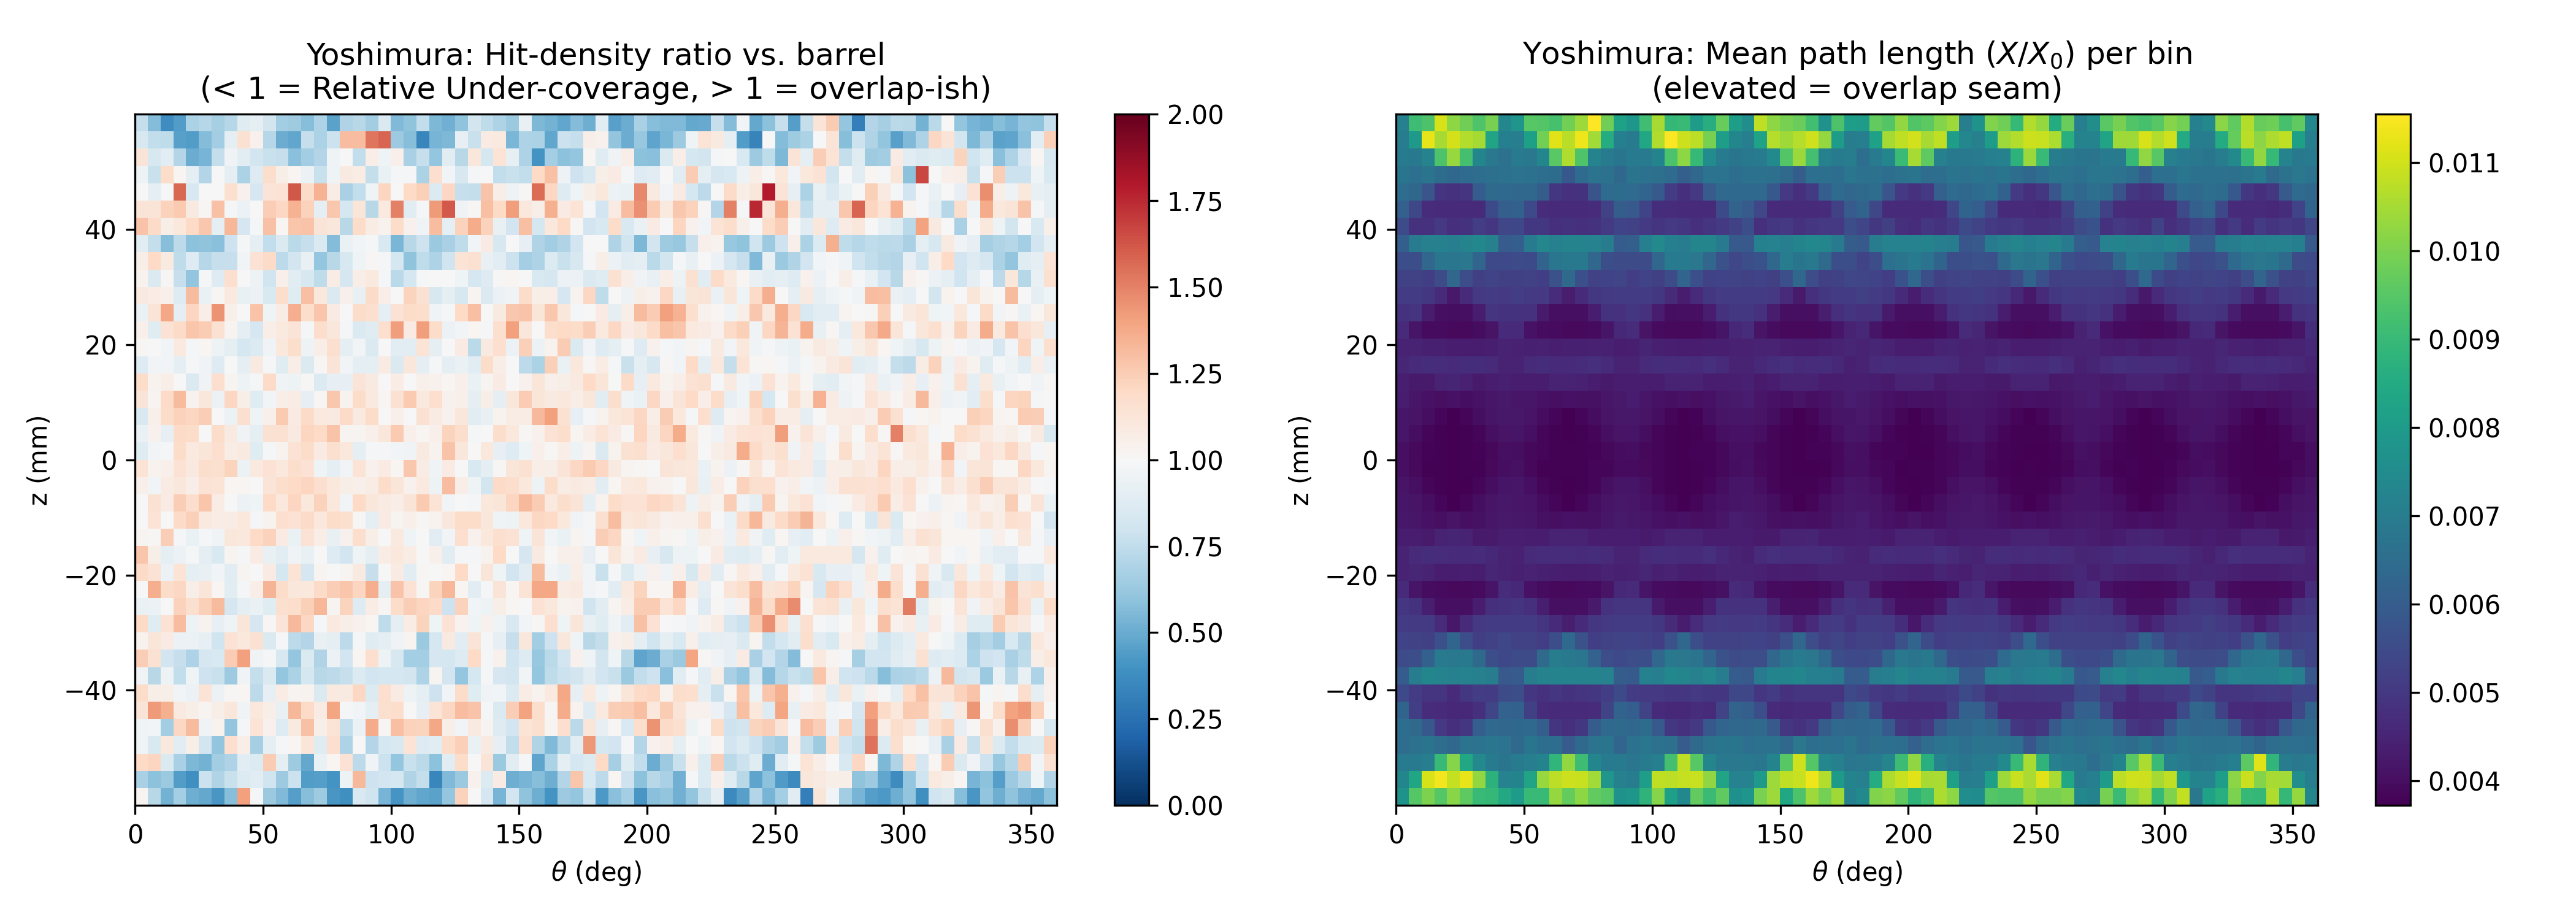
\includegraphics[width=0.86\textwidth]{figures/fig11_map_yoshimura.png}
\caption{Spatial hit-density enhancement ratio $R(\theta, z)$ (left) and mean $X_0$ (right) for Yoshimura relative to the barrel control.}
\label{fig:map_yoshimura}
\end{figure}

\begin{figure}[!htbp]
\centering
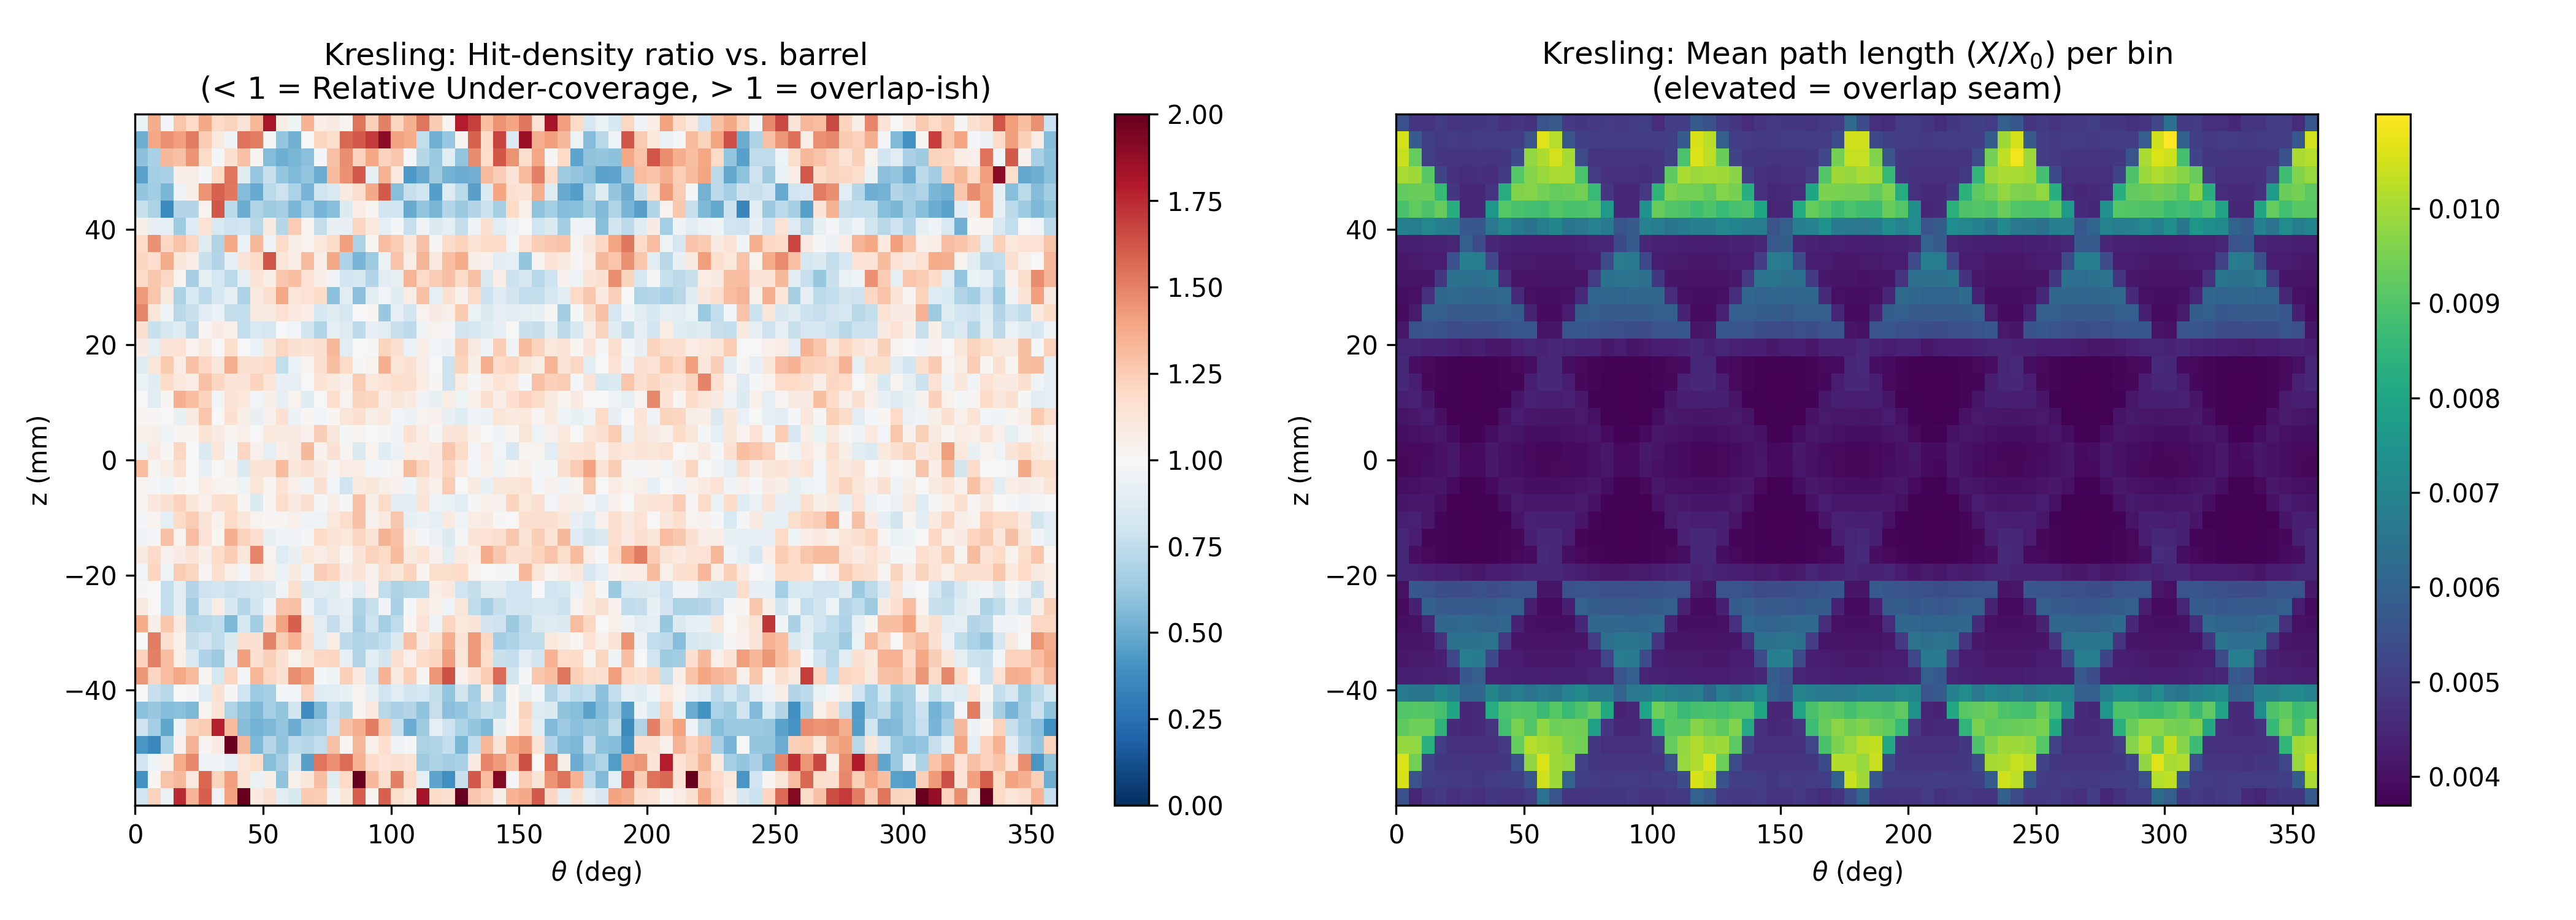
\includegraphics[width=0.86\textwidth]{figures/fig12_map_kresling.png}
\caption{Spatial hit-density enhancement ratio $R(\theta, z)$ (left) and mean $X_0$ (right) for Kresling relative to the barrel control.}
\label{fig:map_kresling}
\end{figure}

\FloatBarrier
\subsection{Path Length vs.\ Local Incidence Angle}
\label{sec:path_length_incidence}

Binned path lengths as a function of local incidence angle $\theta_{\text{local}}$ (Table~\ref{tab:incidence_angle}) confirm textbook $1/\cos(\theta_{\text{local}})$ scaling near normal incidence ($5^\circ$--$25^\circ$), where all geometries match within $0.3\%$. At grazing angles ($\ge 55^\circ$), fold-line seam traversals induce severe non-linear path length growth, with Kresling exceeding the planar barrel baseline by $+27.1\%$ at $65^\circ$ ($0.00796\ X_0$ vs.\ $0.00627\ X_0$), while origami folds maintain active hit coverage out to $75^\circ$--$85^\circ$ where the flat barrel ceases to capture tracks.

\begin{table}[!htbp]
\centering
\caption{Mean path length in $X_0$ across local incidence angle bins $\theta_{\text{local}}$.}
\label{tab:incidence_angle}
\smallskip
\begin{tabular}{ccccc}
\toprule
$\theta_{\text{local}}$ & Barrel $X_0$ & Miura-ori $X_0$ & Kresling $X_0$ & Yoshimura $X_0$ \\
\midrule
$5^\circ$  & 0.003384 & 0.003392 & 0.003382 & 0.003390 \\
$15^\circ$ & 0.003480 & 0.003481 & 0.003478 & 0.003487 \\
$25^\circ$ & 0.003710 & 0.003704 & 0.003708 & 0.003708 \\
$35^\circ$ & 0.004105 & 0.004095 & 0.004061 & 0.004089 \\
$45^\circ$ & 0.004750 & 0.004747 & 0.004692 & 0.004642 \\
$55^\circ$ & 0.005578 & 0.005639 & 0.005599 & 0.005898 \\
$65^\circ$ & 0.006268 & 0.006973 & 0.007964 & 0.007408 \\
$75^\circ$ & ---       & 0.007162 & 0.010032 & 0.009871 \\
$85^\circ$ & ---       & ---       & ---       & 0.009458 \\
\bottomrule
\end{tabular}
\end{table}

\paragraph{Fiducial vs.\ peripheral acceptance decomposition.}
Table~\ref{tab:incidence_angle} shows that the flat barrel ceases to capture tracks beyond $\theta_{\text{local}} \approx 65^\circ$, while fold geometries extend coverage to $75^\circ$--$85^\circ$. To quantify how much of the global acceptance gain arises from this extended angular reach at the barrel ends versus from seam redistribution within the central tracking region, the primary event sample was partitioned using a geometry-independent fiducial cut on the generated track direction.

The central fiducial region is defined as $|\eta| \le 0.80$, corresponding to primary emission polar angles $\theta \in [48.39^\circ, 131.61^\circ]$, which encloses a fraction $f_{\text{fid}} = (\cos 48.39^\circ - \cos 131.61^\circ)/2 \approx 0.6638$ of the isotropic $4\pi$ solid angle. Each primary pion is classified into either the central fiducial band or the peripheral band ($|\eta| > 0.80$) based on its true generated emission polar angle ($\theta$). The fiducial acceptance $A_{\text{fid}}$ is evaluated as the measured hit count within the band divided by the measured number of primaries generated into that band ($N_{\text{gen, fid}} \approx 332{,}000$ per run), guaranteeing $A_{\text{fid}} \le 1.0$ by construction; the peripheral acceptance $A_{\text{periph}}$ is evaluated analogously. Table~\ref{tab:fiducial_decomp} reports the results averaged across all five independent simulation runs.

\begin{table}[!htbp]
\centering
\caption{Fiducial ($|\eta| \le 0.80$, $\theta \in [48.39^\circ, 131.61^\circ]$) vs.\ peripheral ($|\eta| > 0.80$) acceptance decomposition, averaged across five independent runs. $A_{\text{fid}}$ and $A_{\text{periph}}$ are evaluated per run as $N_{\text{hit}} / N_{\text{gen}}$ using the actual simulated primary counts in each band; $\Delta A$ values are differences vs.\ the fine-tiled barrel. The rightmost column gives the fraction of the global acceptance gain attributable to the peripheral band ($f_{\text{periph}} \Delta A_{\text{periph}} / \Delta A_{\text{global}}$).}
\label{tab:fiducial_decomp}
\smallskip
\resizebox{\textwidth}{!}{
\begin{tabular}{lccccccc}
\toprule
Geometry & $A_{\text{global}}$ & $\Delta A_{\text{global}}$ (pp) & $A_{\text{fid}}$ & $\Delta A_{\text{fid}}$ (pp) & $A_{\text{periph}}$ & $\Delta A_{\text{periph}}$ (pp) & Peripheral share \\
\midrule
Barrel (fine)  & 0.8318 & ---     & 0.9998 & ---     & 0.5002 & ---     & ---   \\
Miura-ori      & 0.8367 & $+0.49$ & 0.9998 & $+0.00$ & 0.5141 & $+1.39$ & 94.4\% \\
Kresling       & 0.8554 & $+2.36$ & 0.9998 & $+0.00$ & 0.5689 & $+6.87$ & 97.5\% \\
Yoshimura      & 0.8448 & $+1.30$ & 0.9998 & $+0.00$ & 0.5386 & $+3.84$ & 98.9\% \\
\bottomrule
\end{tabular}
}
\end{table}

The decomposition reveals that within the central fiducial region, all four geometries achieve identical near-hermetic acceptance ($A_{\text{fid}} = 99.98\%$). The fold seams in the three origami designs do not introduce measurable inactive voids in the central tracking volume. Consequently, the global acceptance advantage of the fold geometries is overwhelmingly peripheral: $94.4\%$ of Miura-ori's acceptance gain, $97.5\%$ of Kresling's acceptance gain, and $98.9\%$ of Yoshimura's acceptance gain arises from the peripheral band ($|\eta| > 0.80$). This separates two distinct geometric regimes: within the central barrel volume, flat tiles and folded facets perform identically, while at large pseudorapidity ($|\eta| > 0.80$), inclined end facets capture grazing tracks ($\theta_{\text{local}} \gtrsim 65^\circ$) that escape uninstrumented past the boundaries of the flat barrel.

\subsection{Thin-Silicon Variant (50 \texorpdfstring{$\mu$}{u}m) and Comparison to ITS3}
\label{sec:thin_silicon}

The results in Sections~\ref{sec:headline_results}--\ref{sec:path_length_incidence} use the nominal $300\text{ }\mu\text{m}$ silicon thickness given in Table~\ref{tab:geom_params}. To check how the results change for a thinner sensor, all four geometries were also simulated with the silicon thickness reduced to $50\text{ }\mu\text{m}$. This thickness is comparable to the $40$--$50\text{ }\mu\text{m}$ silicon used for the ALICE ITS3 sensors~\cite{ALICE2024, Sonneveld2023}.

For this comparison, the radius, active length, Kapton thickness, fold parameters, particle beam, event count, and vertex smear were kept the same as the nominal configuration. This means that the main change between the two cases is the silicon thickness.

Each geometry was simulated using a single $500{,}000$-event run. This follows the single-run treatment used for the headline results in Table~\ref{tab:headline_results} rather than the five-run replication used in Tables~\ref{tab:multirun_results} and~\ref{tab:deadzone_multirun}. The acceptance comparisons therefore use the binomial standard errors and $z$-tests described in Section~\ref{sec:statistics}, rather than the Welch's $t$-test used for the five-run results. Since only one run was performed at $50\text{ }\mu\text{m}$, run-to-run variation at this thickness has not been measured.

\subsubsection{Headline performance at 50 \texorpdfstring{$\mu$}{u}m}

Table~\ref{tab:thin_silicon_headline} shows the acceptance and mean radiation-length traversal for the four geometries with $50\text{ }\mu\text{m}$ silicon.

\begin{table}[!htbp]
\centering
\caption{Single-run headline performance at $50\text{ }\mu\text{m}$ silicon ($500{,}000$ primaries each).}
\label{tab:thin_silicon_headline}
\smallskip
\resizebox{\textwidth}{!}{
\begin{tabular}{lcccccc}
\toprule
Geometry & Hits / Total & Acceptance & Mean $X/X_0$ & 95\% CI & Median $X/X_0$ & IQR \\
\midrule
Barrel (fine) & 415,826 / 500,000 & 0.831652 & 0.000840 & [0.000839, 0.000840] & 0.000782 & 0.000182 \\
Miura-ori     & 418,769 / 500,000 & 0.837538 & 0.000850 & [0.000849, 0.000850] & 0.000786 & 0.000183 \\
Kresling      & 427,686 / 500,000 & 0.855372 & 0.000868 & [0.000867, 0.000869] & 0.000777 & 0.000175 \\
Yoshimura     & 422,135 / 500,000 & 0.844270 & 0.000894 & [0.000893, 0.000895] & 0.000817 & 0.000193 \\
\bottomrule
\end{tabular}
}
\end{table}

All three origami geometries again give higher acceptance than the fine-tiled barrel. Kresling gives the largest increase, followed by Yoshimura and Miura-ori.

The pairwise comparisons in Table~\ref{tab:thin_silicon_pairwise} show that all three acceptance gains remain statistically significant.

\begin{table}[!htbp]
\centering
\caption{Pairwise acceptance and material-cost comparisons vs.\ barrel, $50\text{ }\mu\text{m}$ silicon (single run, $z$-test per Eqs.~\ref{eq:se_binomial}--\ref{eq:z_score}). Following Section~\ref{sec:statistics}, Holm--Bonferroni correction is applied across the three comparisons.}
\label{tab:thin_silicon_pairwise}
\smallskip
\resizebox{\textwidth}{!}{
\begin{tabular}{lccccccc}
\toprule
Comparison & $\Delta A$ (pp) & $z$ & $p$ & Holm thresh. & Sig.? & Cohen's $h$ & $\Delta X_0$ (\%) \\
\midrule
Barrel vs.\ Kresling  & $+2.372$ & $32.66$ & $<10^{-16}$           & $0.0167$ & Yes & $+0.065$ & $+3.38\%$ \\
Barrel vs.\ Yoshimura & $+1.262$ & $17.12$ & $<10^{-16}$           & $0.025$  & Yes & $+0.034$ & $+6.49\%$ \\
Barrel vs.\ Miura-ori & $+0.589$ & $7.92$  & $2.4\times 10^{-15}$  & $0.05$   & Yes & $+0.016$ & $+1.21\%$ \\
\bottomrule
\end{tabular}
}
\end{table}

The ordering is therefore the same as at $300\text{ }\mu\text{m}$. Kresling provides the largest acceptance gain, Yoshimura provides the second largest, and Miura-ori provides the smallest gain. The material penalty is also still smallest for Miura-ori.

\subsubsection{Effect of silicon thickness on acceptance}

Table~\ref{tab:thin_silicon_thickness_comparison} compares the acceptance gain over the barrel at $300\text{ }\mu\text{m}$ and $50\text{ }\mu\text{m}$ silicon.

\begin{table}[!htbp]
\centering
\caption{Acceptance gain over barrel, $300\text{ }\mu\text{m}$ vs.\ $50\text{ }\mu\text{m}$ silicon.}
\label{tab:thin_silicon_thickness_comparison}
\smallskip
\begin{tabular}{lcc}
\toprule
Geometry  & $\Delta A$ at $300\text{ }\mu\text{m}$ (pp) & $\Delta A$ at $50\text{ }\mu\text{m}$ (pp) \\
\midrule
Miura-ori & $+0.493$ & $+0.589$ \\
Kresling  & $+2.362$ & $+2.372$ \\
Yoshimura & $+1.304$ & $+1.262$ \\
\bottomrule
\end{tabular}
\end{table}

The acceptance gains are very similar at the two silicon thicknesses. Kresling changes by only $0.010$ percentage points, Yoshimura by $-0.042$ percentage points, and Miura-ori by $+0.096$ percentage points.

These differences are small compared with the run-to-run spread measured for the $300\text{ }\mu\text{m}$ simulations in Table~\ref{tab:multirun_results}, where $\mathrm{SD}_A \leq 0.05\text{ pp}$. This suggests that the acceptance difference between the geometries is mainly controlled by the geometry of the facets, seams, and under-coverage regions rather than by the silicon thickness.

However, this should not be treated as a full statistical demonstration of thickness independence. Only one run was performed at $50\text{ }\mu\text{m}$. A five-run replication at $50\text{ }\mu\text{m}$ would be needed to measure the run-to-run variation directly.

The material traversal changes much more strongly when the silicon thickness is reduced. The mean $X/X_0$ decreases by approximately $4.74$--$4.84\times$ across the four geometries. The reduction is smaller than the factor of six expected from the silicon thickness alone, since the Kapton layer remains at $50\text{ }\mu\text{m}$ in both simulations and therefore accounts for a larger share of the total material at $50\text{ }\mu\text{m}$ silicon.

\subsubsection{Comparison to ALICE ITS3}

The ALICE ITS3 detector provides a useful reference for the $50\text{ }\mu\text{m}$ case. However, two different material-budget numbers are used for ITS3 and they describe different parts of the detector.

The silicon sensor itself contributes approximately $0.053\%\ X_0$. The full engineered layer, including the silicon together with carbon-foam stiffeners, structural glue, and air cooling, is approximately $0.09\%\ X_0$~\cite{ALICE2024, Sonneveld2023}.

These two values should therefore not be treated as two estimates of the same quantity. The $0.053\%\ X_0$ value describes the silicon only, while the $0.09\%\ X_0$ value describes a larger part of the detector structure.

The simulation in this project contains silicon and Kapton only. Table~\ref{tab:thin_silicon_its3_comparison} therefore compares the silicon part of the simulation with the ITS3 silicon-only value, and the complete simulated silicon + Kapton stack with the full ITS3 layer budget.

\begin{table}[!htbp]
\centering
\caption{Mean $X/X_0$ at $50\text{ }\mu\text{m}$ silicon compared with the two ITS3 reference values.}
\label{tab:thin_silicon_its3_comparison}
\smallskip
\resizebox{\textwidth}{!}{
\begin{tabular}{lcccc}
\toprule
Geometry & Si-only $X/X_0$ & Difference from ITS3 Si-only ($0.053\%$) & Si+Kapton $X/X_0$ & Difference from ITS3 full budget ($0.09\%$) \\
\midrule
Barrel (fine) & $0.0633\%$ & $+0.0103\text{ pp}$ & $0.0840\%$ & $-0.0060\text{ pp}$ \\
Miura-ori     & $0.0646\%$ & $+0.0116\text{ pp}$ & $0.0850\%$ & $-0.0050\text{ pp}$ \\
Kresling      & $0.0674\%$ & $+0.0144\text{ pp}$ & $0.0868\%$ & $-0.0032\text{ pp}$ \\
Yoshimura     & $0.0688\%$ & $+0.0158\text{ pp}$ & $0.0894\%$ & $-0.0006\text{ pp}$ \\
\bottomrule
\end{tabular}
}
\end{table}

\begin{figure}[!htbp]
\centering
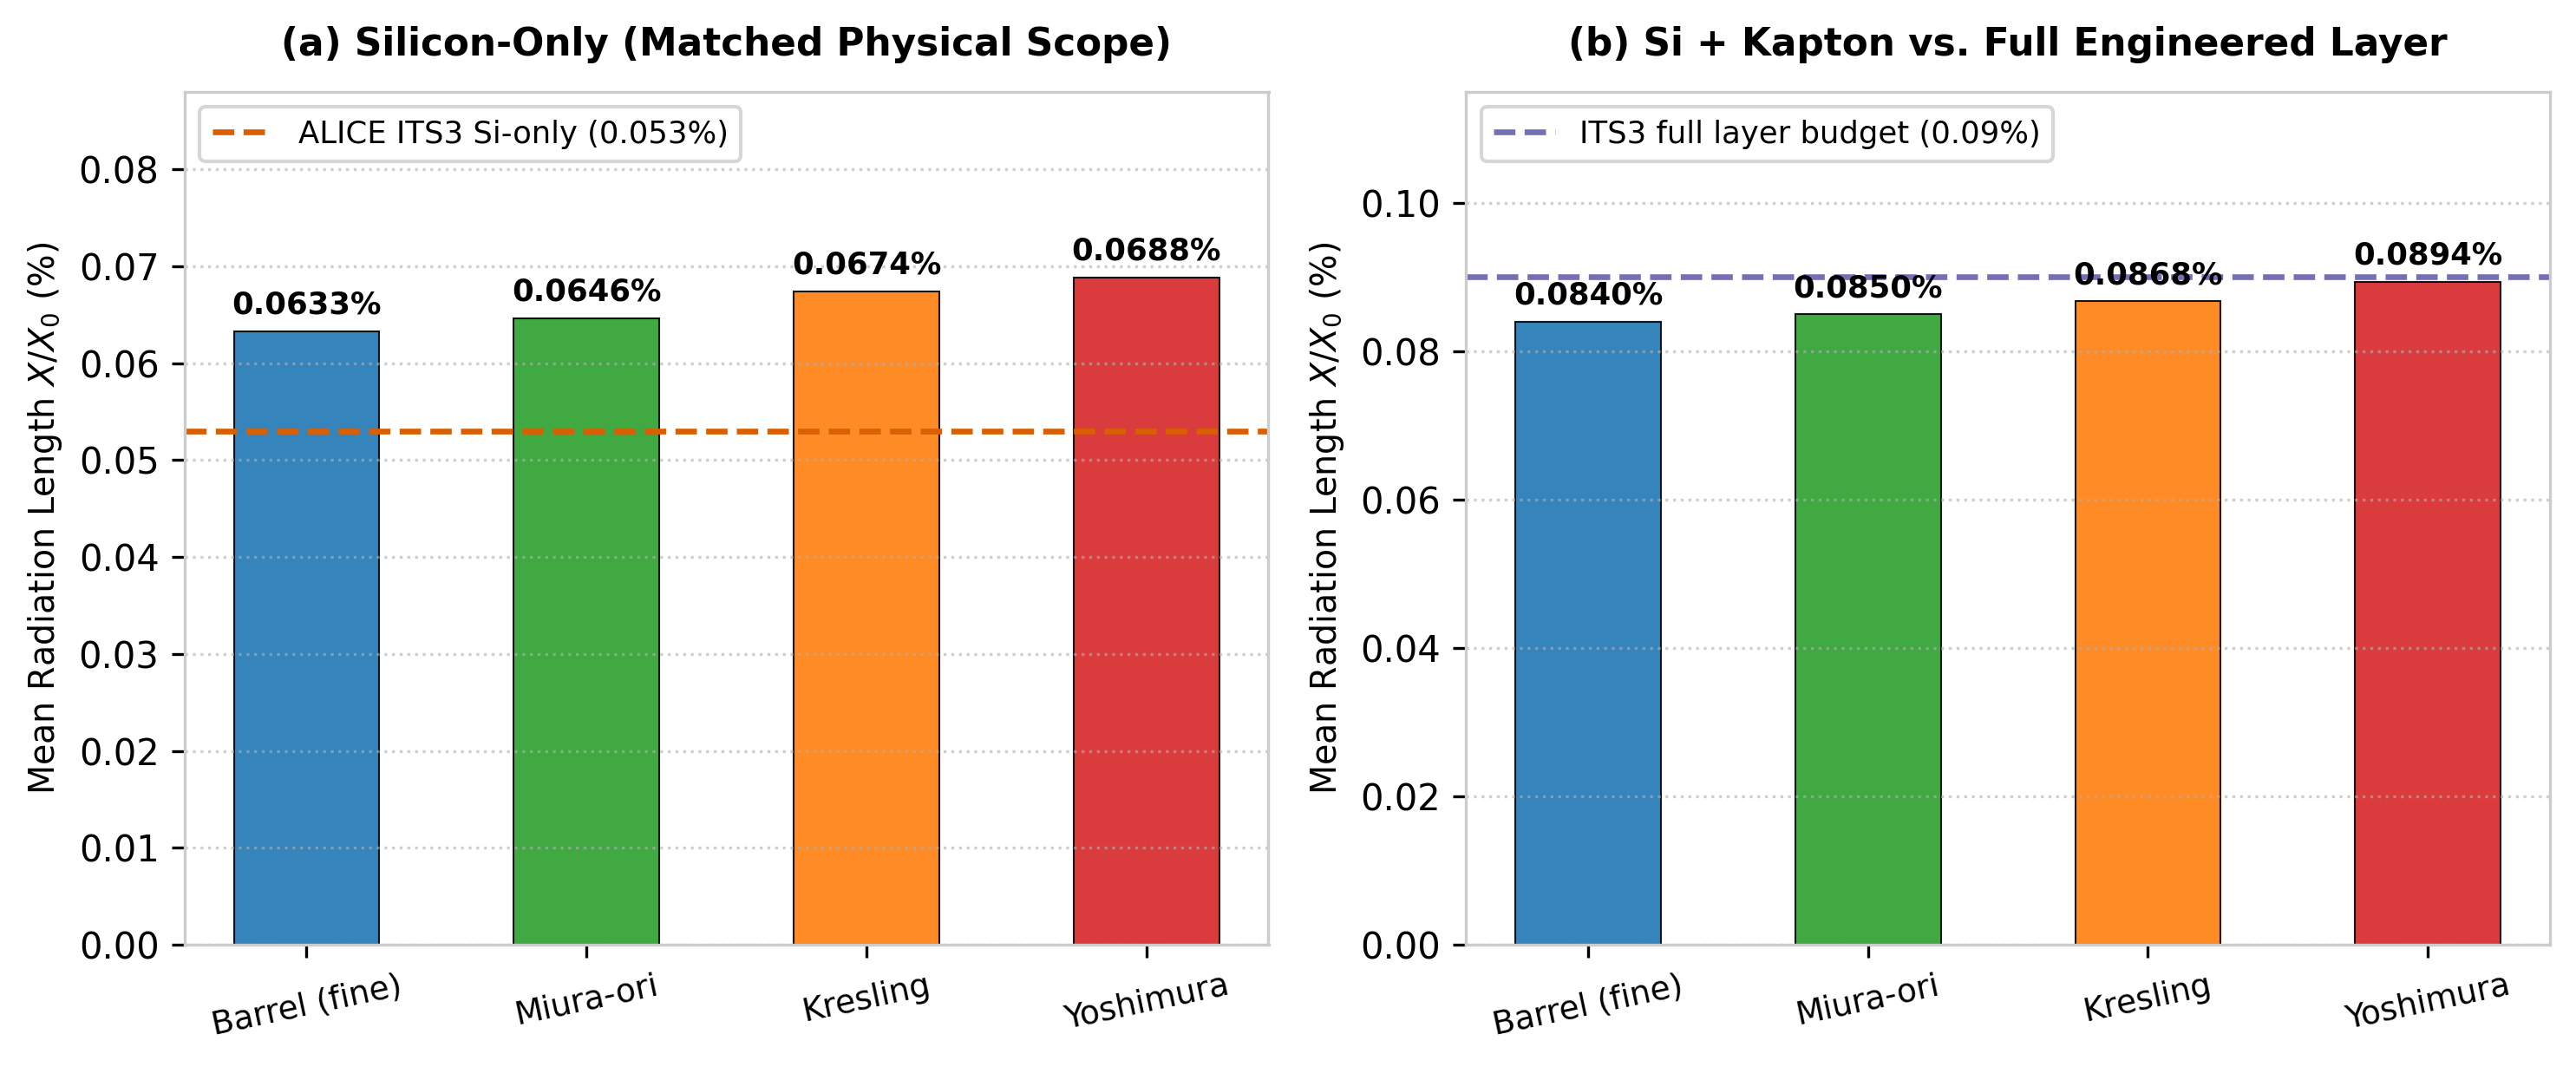
\includegraphics[width=0.96\textwidth]{figures/fig_its3_comparison_v2.png}
\caption{Comparison of mean radiation length $X/X_0$ at $50\text{ }\mu\text{m}$ silicon against ALICE ITS3 benchmark references~\cite{ALICE2024, Sonneveld2023}: (a) silicon-only traversal evaluated at matched physical scope against the ITS3 bent sensor baseline ($0.053\%\ X_0$), and (b) simulated silicon + Kapton stack compared with the full engineered ITS3 layer budget ($0.09\%\ X_0$, which includes carbon-foam supports, glue, and cooling not modeled here).}
\label{fig:its3_comparison}
\end{figure}

The silicon-only comparison is more direct, as both values describe the same physical component. All four geometries have a higher silicon-only material traversal than the ITS3 value, with the difference ranging from $0.010$ to $0.016$ percentage points.

This difference is mainly related to the way the sensor surface is constructed. ITS3 uses very thin silicon that can be bent into a cylindrical shape. A track crossing the sensor therefore sees a surface that follows the cylindrical envelope more closely. The geometries in this project instead use flat silicon facets at a fixed radius. Tracks that do not cross these facets close to normal incidence therefore travel through a longer silicon path.

This effect is also seen in the $300\text{ }\mu\text{m}$ results in Section~\ref{sec:path_length_incidence}, where path length increases with local incidence angle. The fold geometries do not remove this effect. Yoshimura shows the largest silicon-only material traversal of the four geometries, consistent with its larger facet inclination angles.

The second comparison, using silicon plus Kapton, gives a different result. All four simulated geometries are below the $0.09\%\ X_0$ ITS3 full-layer value. However, this is not a direct material-budget comparison.

The ITS3 full-layer value includes structural components such as carbon-foam stiffeners and structural glue, while the present simulation includes only a $50\text{ }\mu\text{m}$ Kapton backing. Mechanical supports, glue, cooling, cabling, and readout electronics are not included in this model, as described in Sections~\ref{sec:intro} and~\ref{sec:limitations}. The Kapton layer is therefore a much simpler and lighter representation of the detector structure.

The fact that the simulated silicon + Kapton values are below $0.09\%\ X_0$ should therefore not be interpreted as showing that the folded geometries have a lower material budget than ITS3. The two simulations do not contain the same structural components.

Overall, the $50\text{ }\mu\text{m}$ comparison shows that reducing the silicon thickness substantially reduces the material traversal while leaving the acceptance advantage of the folded geometries almost unchanged. The folded geometries do not, however, achieve a lower silicon-only material traversal than the ITS3 sensor.

The main result of the folding approach therefore remains the same as in the $300\text{ }\mu\text{m}$ study. Folding can increase geometric acceptance relative to a flat-tiled barrel, but this comes with an increase in material traversal. At $50\text{ }\mu\text{m}$, Kresling again gives the largest acceptance gain, while Miura-ori remains the closest to the barrel in material cost. The comparison with ITS3 also shows the limitation of this approach: a bent, seamless sensor can reduce the path-length penalty that remains when a cylindrical surface is approximated using flat silicon facets.

\FloatBarrier
\section{Discussion}
\label{sec:discussion}
The simulation results indicate that no single fold geometry strictly outperforms the others across all metrics; instead, the candidate designs form a distinct Pareto frontier. The central finding of this study is that origami folding increases geometric hit acceptance relative to a flat-tiled cylinder of identical envelope, but this gain is accompanied by an increase in mean radiation-length traversal. The spatial distribution of this trade-off differs across the three fold families.

Yoshimura and Kresling concentrate their acceptance gains primarily in localized seam-overlap regions, which leads to higher relative under-coverage fractions ($1.86\%$ and $1.45\%$, respectively) in intermediate areas. Miura-ori, by contrast, exhibits the lowest material penalty ($+1.88\%$ in mean $X_0$) while delivering a reliable acceptance increase ($+0.49$ pp, $t = -23.44$, $p < 10^{-7}$) and the lowest relative under-coverage fraction ($0.04\%$), maintaining a spatial hit distribution close to the control barrel.

Kresling achieves the highest overall acceptance gain over the flat barrel ($+2.36$ pp, $t = -128.89$), but incurs a $+5.69\%$ increase in mean $X_0$. Yoshimura exhibits an intermediate acceptance gain ($+1.30$ pp), yet imposes both the highest radiation-length penalty ($+8.01\%$) and the largest under-coverage fraction ($1.86\%$). Consequently, Yoshimura is disadvantaged under standard cylindrical packaging constraints when compared directly with Kresling. As demonstrated by the parameter sweeps (Sections~\ref{sec:n_sweep}--\ref{sec:theta_sweep}), Yoshimura's nominal fold angle ($\theta = 30^\circ$) already operates in the lower-material regime of its design space, and further increasing $\theta$ rapidly increases material traversal without closing this efficiency gap.

The practical selection therefore narrows to a trade-off between Miura-ori and Kresling:
\begin{itemize}
    \item \textbf{Acceptance-limited applications} requiring maximum geometric coverage favor \textbf{Kresling} ($+2.36$ pp gain), provided that tracking algorithms can handle localized material increases near vertex nodes.
    \item \textbf{Momentum-resolution-limited applications} where multiple scattering dominates track uncertainties favor \textbf{Miura-ori}, which offers minimal material inflation ($+1.88\%$) and a spatially uniform response.
\end{itemize}

The thin-silicon evaluation at $50\ \mu\text{m}$ (Section~\ref{sec:thin_silicon}) confirms that these geometric trade-offs remain consistent at lower sensor thickness: reducing the sensor thickness by a factor of six scales the total material traversal down by $\sim 4.8\times$ while preserving relative acceptance differences ($+2.37$ pp for Kresling, $+1.26$ pp for Yoshimura, and $+0.59$ pp for Miura-ori). When benchmarked against the ALICE ITS3 bent-sensor architecture at matched physical scope, flat-faceted origami tessellations maintain a small silicon-only material excess ($+0.010$--$0.016$ pp in $X/X_0$) due to non-normal local track incidence on inclined facets.

In summary, origami folding does not eliminate the fundamental under-coverage and overlap trade-off; rather, it redistributes the geometric response across distinct Pareto-optimal configurations.

\section{Limitations and Future Work}
\label{sec:limitations}

This study focuses on radiation transport and geometric acceptance. Several practical engineering aspects remain outside the scope of this work:
\begin{enumerate}
    \item \textbf{Structural and thermo-mechanical performance:} Fold-vertex stress concentrations, thermal dissipation pathways, and structural stability under gravitational and magnetic loads require dedicated mechanical modeling and modal testing.
    \item \textbf{Complete detector material budget:} Auxiliary components --- including structural glue layers, wire bonds, cooling ducts, power distribution buses, and readout ASICs --- were omitted to cleanly isolate pure geometric effects. Incorporating these subsystems will require dedicated engineering design.
    \item \textbf{Physical prototyping:} Fabricating functional, flexible silicon-on-substrate origami assemblies and evaluating them in test beams represent the primary next steps for technology validation.
\end{enumerate}

\section{Conclusion}
\label{sec:conclusion}

This study compared three cylindrically deployable origami fold patterns --- Cylindrical Miura-ori~\cite{Miura1985}, Yoshimura~\cite{Yoshimura1955}, and Kresling~\cite{Kresling2008} --- with a conventional flat-tiled barrel tracking detector of identical bounding envelope ($R = 40\text{ mm}$, $L = 120\text{ mm}$). Simulations were performed within a differentiated-material \textsc{Geant4} framework with $5\text{ GeV}/c\ \pi^+$ tracks, evaluating hit acceptance, radiation-length traversal, spatial uniformity, and multiple Coulomb scattering.

The primary conclusions are as follows:
\begin{enumerate}
    \item \textbf{Pareto trade-off surface:} Origami folding consistently increases geometric hit acceptance relative to a flat-tiled cylinder, accompanied by an increase in material traversal. Kresling maximizes acceptance ($+2.36$ pp, $+5.69\%$ $X_0$), Miura-ori minimizes material excess ($+0.49$ pp, $+1.88\%$ $X_0$), and Yoshimura incurs a higher material penalty for its gain ($+1.30$ pp, $+8.01\%$ $X_0$).
    \item \textbf{Spatial and angular decomposition:} Fiducial decomposition indicates that the majority of Kresling's and Yoshimura's global acceptance gains arise from extended angular capture of grazing-angle tracks at the cylinder boundaries ($|\eta| > 0.80$), while all geometries maintain near-hermetic efficiency ($A_{\text{fid}} \ge 99.9\%$) within the central tracking region.
    \item \textbf{Consistency across sensor thickness:} The geometric acceptance hierarchy is preserved when scaling silicon thickness down to $50\ \mu\text{m}$, while reducing total material traversal by $\sim 4.8\times$.
\end{enumerate}

This work provides what appears to be the first systematic \textsc{Geant4} comparison of cylindrically deployable origami geometries against a conventional tiled detector baseline. These results establish origami tessellation as a viable and mathematically rigorous design approach for future deployable tracking detectors.
\acknowledgments
The author thanks Prof. Biplob Bhattacharjee for his valuable feedback on the initial idea for this work. Thank you to Professor Mei Dongming at the University of South Dakota for his feedback. The author is deeply grateful to his parents for their unwavering support, encouragement, and patience throughout the course of this work, and for making it possible to pursue it in the first place. Claude (Anthropic) was used as an auxiliary tool for debugging and troubleshooting code during the development of the simulation and analysis pipeline.

\appendix

\section{Full Multiple-Scattering Validation Dataset}
\label{sec:appendix_highland}

\begin{table}[!htbp]
\centering
\caption{Full multiple-scattering dataset (all four geometries $\times$ five beam momenta, 20 points), Rayleigh-core-plus-Rutherford-tail mixture fit to the space-scattering angle (\texttt{scatterAngleDeg}), fit by unbinned maximum likelihood (Section~\ref{sec:validation}). $\sigma$ is the fitted Rayleigh core scale, directly comparable to Highland's projected $\theta_0$ with no additional conversion factor; $\theta_{0,\text{Highland}}$ is the Highland-formula prediction (Eq.~\ref{eq:highland}) at the same momentum and mean $x/X_0$; $\alpha$ is the fitted tail power index (Rutherford single-scattering prediction: $\alpha = 3$); tail fraction is the share of events beyond the fitted tail-onset boundary $\theta_{\min} = 3\sigma$. Binned $\chi^2/\text{dof}$ values are calculated over fine log-bins and reflect the high statistical sensitivity ($N \approx 4.2 \times 10^5$) of the full event sample.}
\label{tab:highland_mixture_fits}
\label{tab:table11}
\small
\resizebox{\textwidth}{!}{%
\begin{tabular}{lcccccccc}
\toprule
Geometry & $p$ (GeV/$c$) & $N_{\text{hit}}$ & $\sigma$ (deg) & $\theta_{0,\text{Highland}}$ (deg) & $\sigma/\theta_{0,\text{Highland}}$ & Tail fraction & Tail index $\alpha$ & $\chi^2/\text{dof}$ (binned) \\
\midrule
Barrel reference & 0.5 & 415,207 & 0.07491 & 0.08008 & 0.935 & 3.29\% & 2.908 & 59.89 \\
Barrel reference & 1.0 & 415,763 & 0.03626 & 0.03894 & 0.931 & 3.44\% & 2.960 & 40.59 \\
Barrel reference & 2.0 & 415,408 & 0.01799 & 0.01933 & 0.931 & 3.50\% & 2.932 & 31.18 \\
Barrel reference & 5.0 & 415,794 & 0.00715 & 0.00772 & 0.927 & 3.57\% & 2.993 & 60.90 \\
Barrel reference & 10.0 & 416,043 & 0.00358 & 0.00386 & 0.928 & 3.65\% & 2.976 & 53.05 \\
\midrule
Kresling & 0.5 & 426,932 & 0.07649 & 0.08211 & 0.932 & 3.68\% & 3.000 & 72.65 \\
Kresling & 1.0 & 427,408 & 0.03695 & 0.03995 & 0.925 & 3.89\% & 3.068 & 38.96 \\
Kresling & 2.0 & 427,092 & 0.01840 & 0.01983 & 0.928 & 3.81\% & 3.041 & 82.45 \\
Kresling & 5.0 & 427,547 & 0.00733 & 0.00792 & 0.925 & 3.93\% & 3.047 & 35.38 \\
Kresling & 10.0 & 427,690 & 0.00366 & 0.00395 & 0.927 & 3.88\% & 3.051 & 46.32 \\
\midrule
Miura-ori & 0.5 & 418,117 & 0.07556 & 0.08081 & 0.935 & 3.33\% & 2.969 & 44.05 \\
Miura-ori & 1.0 & 418,508 & 0.03669 & 0.03930 & 0.934 & 3.45\% & 2.955 & 68.03 \\
Miura-ori & 2.0 & 418,312 & 0.01817 & 0.01951 & 0.931 & 3.51\% & 2.946 & 45.80 \\
Miura-ori & 5.0 & 418,451 & 0.00724 & 0.00779 & 0.930 & 3.50\% & 3.015 & 32.48 \\
Miura-ori & 10.0 & 418,057 & 0.00363 & 0.00389 & 0.932 & 3.50\% & 2.976 & 30.54 \\
\midrule
Yoshimura & 0.5 & 421,642 & 0.07741 & 0.08315 & 0.931 & 3.63\% & 2.973 & 37.94 \\
Yoshimura & 1.0 & 422,099 & 0.03740 & 0.04046 & 0.924 & 3.76\% & 3.068 & 52.99 \\
Yoshimura & 2.0 & 422,310 & 0.01861 & 0.02008 & 0.927 & 3.81\% & 3.027 & 60.63 \\
Yoshimura & 5.0 & 422,587 & 0.00747 & 0.00802 & 0.932 & 3.71\% & 3.024 & 70.42 \\
Yoshimura & 10.0 & 422,058 & 0.00372 & 0.00401 & 0.927 & 3.74\% & 3.041 & 58.37 \\
\bottomrule
\end{tabular}%
}
\end{table}
 
Across all 20 points, $\sigma/\theta_{0,\text{Highland}} = 0.930 \pm 0.003$ (mean $\pm$ population standard deviation), ranging from 0.924 to 0.935; a weak downward trend against momentum does not reach conventional significance at this sample size (Section 2.6). The fitted tail index averages $\alpha = 2.999 \pm 0.046$ --- indistinguishable from the Rutherford-predicted value of 3 to within fit uncertainty --- while the tail's share of the total $\Sigma\theta^2$ averages 86.5\% (range 81.9--89.7\%) despite the tail itself comprising only 3.3--3.9\% of events at any given point. Both properties are visualized directly in Figure~\ref{fig:scattering_mixture_summary}.

\FloatBarrier
\section{Data and Code Availability}
\label{sec:appendix_provenance}

All baseline simulation datasets were generated under the differentiated-mesh \textsc{Geant4} v11.x pipeline utilizing a nominal $3.0\text{ mm}$ 3D Gaussian vertex smear and $500{,}000$ primary $5\text{ GeV}/c\ \pi^+$ events per configuration at the fully deployed nominal state. Parameter sweep evaluations systematically varied facet count $N$, fold angle $\theta$, and vertex smear $\sigma$ around these baseline settings. Replication studies (Tables~\ref{tab:multirun_results} and~\ref{tab:deadzone_multirun}) utilize five independent simulation runs with distinct pseudo-random engine seeds.

The complete simulation source code, parametric geometry generators, automated pipelines, and figure reproduction scripts are openly available in the GitHub repository:
\begin{center}
\url{https://github.com/Alphacodde/Origami-Particle-Detectors-Geometries}
\end{center}
The raw \textsc{Geant4} ROOT ntuple datasets ($> 7\text{ GB}$ across all experiments and sweeps) are archived and accessible via Google Drive:
\begin{center}
\url{https://drive.google.com/drive/folders/1ZbLm0H2FCLPQepytwLGCHj7_VS4sdF78?usp=sharing}
\end{center}

\enlargethispage{2\baselineskip}
\bibliographystyle{JHEP}
\bibliography{biblio}

\end{document}
